%% Aspect ratio 16:10, delete for 4:3
%\documentclass[english, xcolor=table, aspectratio=1610]{beamer}
\documentclass[english, xcolor=table]{beamer}

\usetheme{modernmpibpc}

%% Spacing between itemize items
\newenvironment{itemize1}
{ \begin{itemize}
    \setlength{\itemsep}{8pt}
    \setlength{\parskip}{5pt}
    \setlength{\parsep}{0pt}
}
{ \end{itemize}
}
\newenvironment{itemize2}
{ \begin{itemize}
    \setbeamertemplate{itemize items}[circle]
    \setlength{\itemsep}{5pt}
    \setlength{\parskip}{0pt}
    \setlength{\parsep}{0pt}
}
{ \end{itemize}
}
\newenvironment<>{infoblock}[1]{%
  \vskip 0.1em
  \begin{beamercolorbox}[wd=\textwidth, colsep*=.75ex]{info body}
     \usebeamerfont{info body}#1
  \end{beamercolorbox}
  \vskip 0.5em
}

\usepackage[T1]{fontenc}
%\usepackage{newtxmath}
%\usepackage[varg]{txfonts}
%\usepackage{ccfonts,eulervm}
%\usepackage{kmath,kerkis}
%\usepackage{millennial}
%\usepackage{mathptmx}

\usepackage{fouriernc} % sharper font for on-screen
\DeclareMathAlphabet{\mathbf}{T1}{fut\mathfamilyextension}{b}{n} 
\renewcommand{\bfdefault}{b}
%\setkomafont{sectioning}{\bfseries} % bold titles for fouriernc

%\usepackage[charter]{mathdesign}
\usepackage{charter}
\usepackage[defaultsans]{droidsans}

% Special font for identity matrix
\usepackage{dsfont} 

% Writing equation in box
\usepackage{empheq}
\usepackage[most]{tcolorbox}
\newtcbox{\mymathbox}[1][]{%
    nobeforeafter,
    %math upper,
    %tcbox raise base,
    %enhanced,
    colframe=primary,
    colback=highlight!20,
    boxrule=1pt,
    #1}

% strikeout text
\usepackage{soul}

\usepackage{tikz}
\usetikzlibrary{shapes.geometric, arrows}
\tikzstyle{decision} = [rectangle, rounded corners, minimum width=3cm, minimum height=1cm, line width=1pt, text centered, align=flush center, draw=primary, fill=highlight!20]
\tikzstyle{origin} = [rectangle, rounded corners, minimum width=3cm, minimum height=1cm, line width=1pt, text centered, align=flush center, draw=subdue]%text=secondary]
\tikzstyle{highlight} = [rectangle, rounded corners, minimum width=3cm, minimum height=1cm, line width=1pt, text centered, align=flush center, draw=secondary, fill=important!30]%text=secondary]
\tikzstyle{doubt} = [circle, line width=1pt, text centered, align=flush center, draw=secondary, fill=important!20]
\tikzstyle{arrow} = [thick,->,>=stealth]
\tikzstyle{line} = [thick, -]

%%% text usefuls
\newcommand{\ie}{{\it i.e.\ }}
\newcommand{\eg}{{\it e.g.\ }}
\newcommand{\etal}{{\it et al.\ }}
\newcommand{\ibid}{{\it ibid.\ }}
\newcommand{\cf}{{\it cf.\ }}


\newlength{\mylen}
\newlength{\mycolsep}
\setlength{\mycolsep}{1cm}
\newcommand{\mytwocolumn}[4]{
   \setlength{\mylen}{\dimexpr#1\textwidth-0.5\mycolsep}
   %% \vskip -2em
   \begin{columns}[#2,onlytextwidth]
   \begin{column}{\mylen}
   #3
   \end{column}
   \begin{column}{\dimexpr\textwidth-\mylen-\mycolsep}
   #4
   \end{column}
   \end{columns}}

\newcommand{\myfulltwocolumn}[4]{
   \setlength{\mycolsep}{0em}
   \setlength{\mylen}{\dimexpr#1\textwidth-0.5\mycolsep}
   %% \vskip -2em
   \begin{columns}[#2,onlytextwidth]
   \begin{column}{\mylen}
   #3
   \end{column}
   \begin{column}{\dimexpr\textwidth-\mylen-\mycolsep}
   #4
   \end{column}
   \end{columns}}

\newcommand{\defcolumn}[5]{
   \setlength{\mycolsep}{0em}
   \setlength{\mylen}{\dimexpr#2\textwidth-0.5\mycolsep}
   %% \vskip -2em
   \begin{columns}[#3,onlytextwidth]
   \begin{column}{\mylen}
   {\color{#1} #4}
   \end{column}
   {\color{#1} \vrule{}}
   \begin{column}{\dimexpr\textwidth-\mylen-\mycolsep}
   #5
   \end{column}
   \end{columns}}


\usepackage[absolute,overlay]{textpos}
\newcommand{\references}[1]{%
  \begin{textblock*}{\textwidth}[0,1](0.9em,0.99\textheight)
  \raggedright {\usebeamercolor[fg]{references}\fontsize{7}{7}\selectfont{#1} \par}
  \end{textblock*}
}

\renewenvironment{equation}{%
    \begin{equation*}
}{
    \nonumber 
    \end{equation*}
}

\newcommand\myreference[1]{%
  \begingroup
  \renewcommand\thefootnote{}\footnote{#1}%
  \addtocounter{footnote}{-1}%
  \endgroup
}

\newcommand{\tss}[1]{\ensuremath{^{\text{\kern1pt\scriptsize #1}}}}
\DeclareMathOperator{\logistic}{lf}
\DeclareMathOperator{\Var}{Var}
\DeclareMathOperator{\diag}{diag}
\newcommand{\bs}{\boldsymbol}
\newcommand{\vx}{\mathbf{x}}
\newcommand{\vy}{\mathbf{y}}
\newcommand{\vz}{\mathbf{z}}
\newcommand{\vv}{\mathbf{v}}
\newcommand{\vX}{\mathbf{X}}
\newcommand{\vY}{\mathbf{Y}}
\newcommand{\idop}{\ensuremath{\mathds{I}}}
\newcommand{\idopn}[1]{\ensuremath{\mathds{I}_{#1}}}


\title{Bayesian variable selection logistic regression: multivariate metaanalysis in GWAS}
\author{S. Banerjee \& J. S\"oding}
\institute{Max Planck Institute for Biophysical Chemistry}
\titlegraphic{
\includegraphics[height=1.4cm]{mpi-logo/Max-Planck-Gesellschaft-no-txt.pdf}\nobreak\hspace{1em}%
              
\includegraphics[height=1.4cm]{mpi-logo/Print_Plotter_MPI-BPC_kurz-short_CMYK.eps}}
\date{\today}

\begin{document}

\begin{frame}[label=mytitle]
  \titlepage
\end{frame}

\section{Global}

%\begin{frame}
%  \frametitle{Outline of the talk}
%  \begin{itemize1}
%    \item Overview
%    \item Method // Model and inference
%    \item Simulation results
%    \item Coronary artery diseases (CAD)
%    %\item Future plans
%  \end{itemize1}
%\end{frame}

% \subsection{Overview}
% 
% \begin{frame}
%   \frametitle{Genome-wide association studies (GWAS)}
%   {\center
%     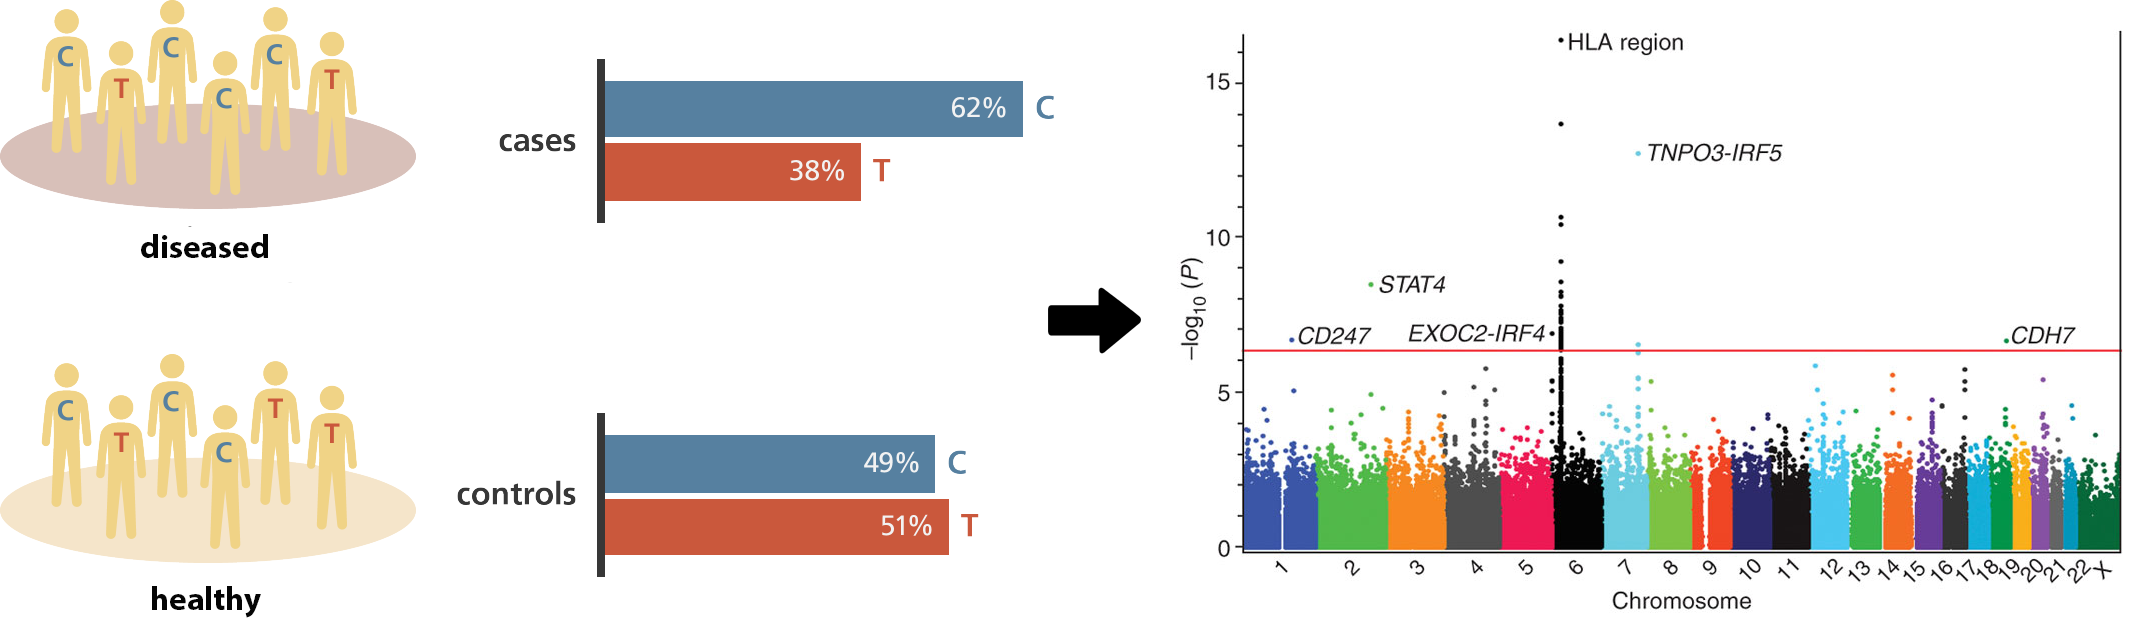
\includegraphics[width=1.0\textwidth]{figures/my_gwas.png}\\
%   }
%   \vskip 0.5em
%   \begin{itemize1}
%     \item Discovered thousands of variants associated with complex diseases
%   \end{itemize1}
%   \myreference{Radstake \etal, \textit{Nat. Gen.} 2010}
% \end{frame}
% 
% \begin{frame}
%   \frametitle{Association tests in GWAS}
%   {\center
%     \vskip -1em
%     \only<1-1>{
%     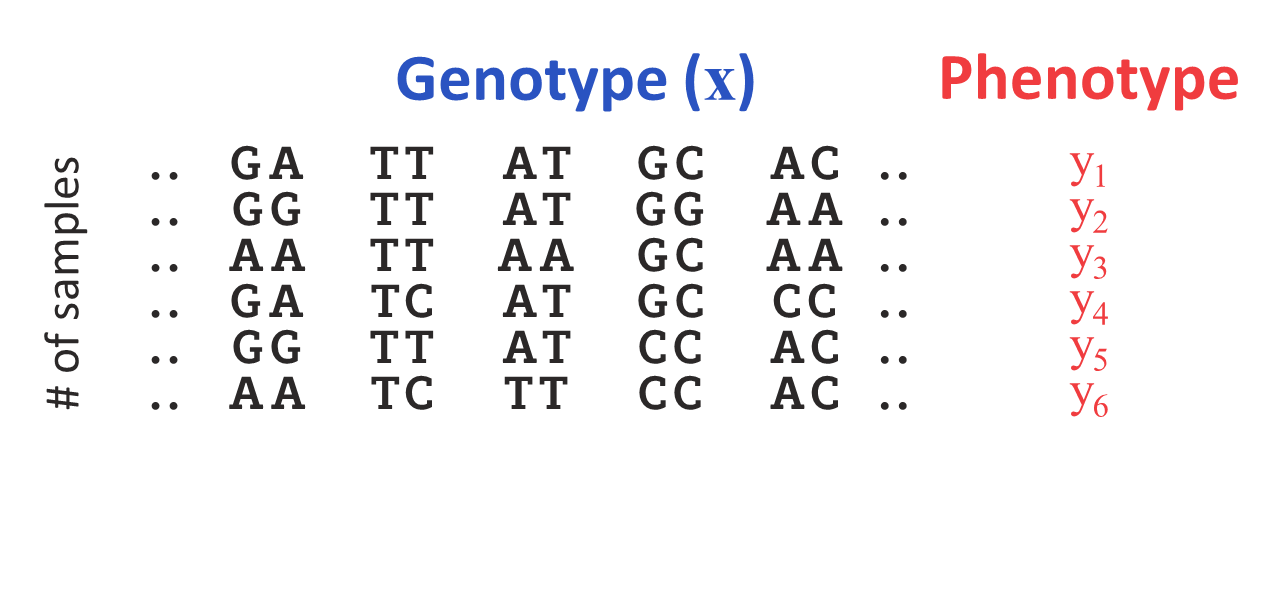
\includegraphics[width=0.6\textwidth]{figures/univariate_model_00.png}\\
%     }
%     \only<2-2>{
%     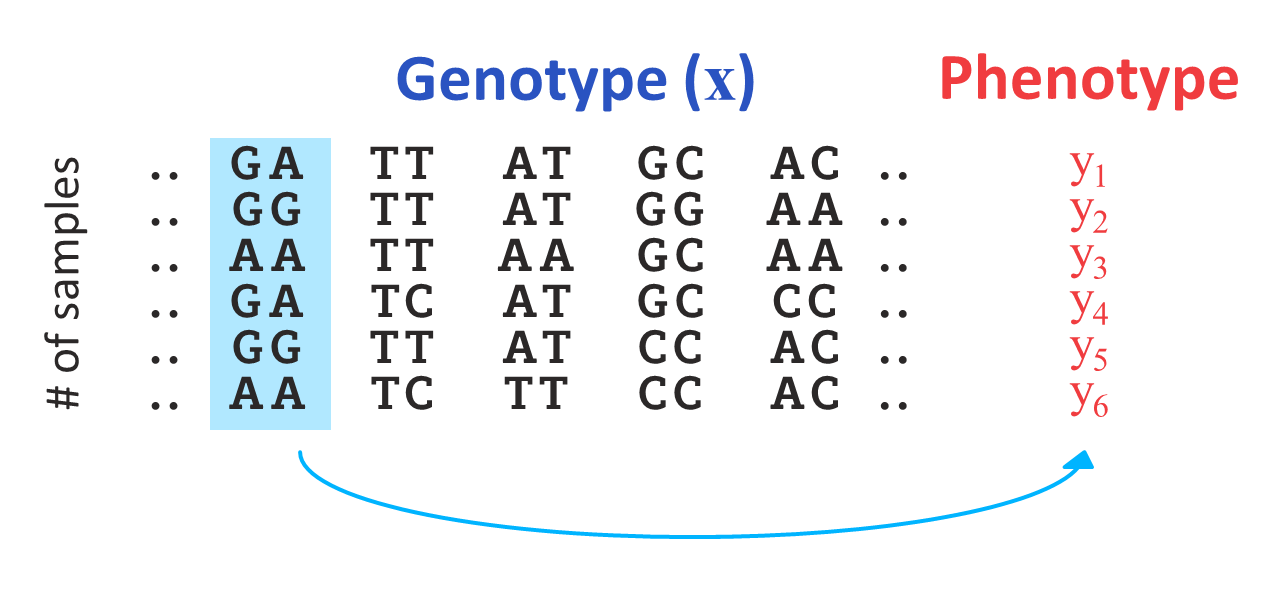
\includegraphics[width=0.6\textwidth]{figures/univariate_model_01.png}\\
%     }
%     \only<3-3>{
%     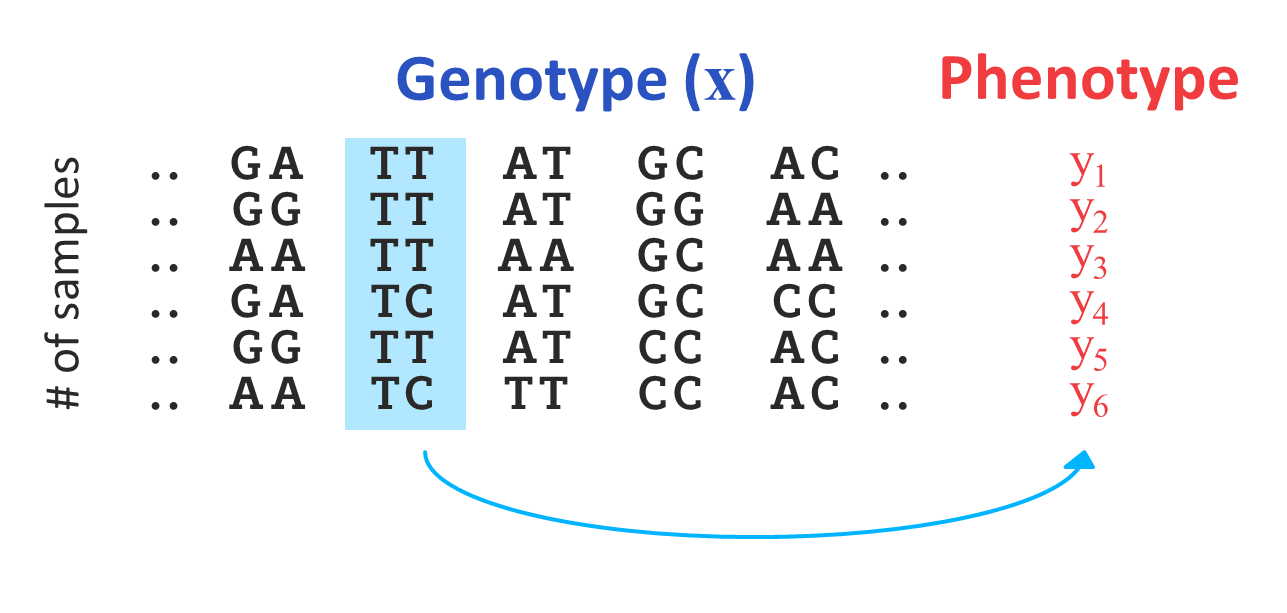
\includegraphics[width=0.6\textwidth]{figures/univariate_model_02.png}\\
%     }
%     \only<4->{
%     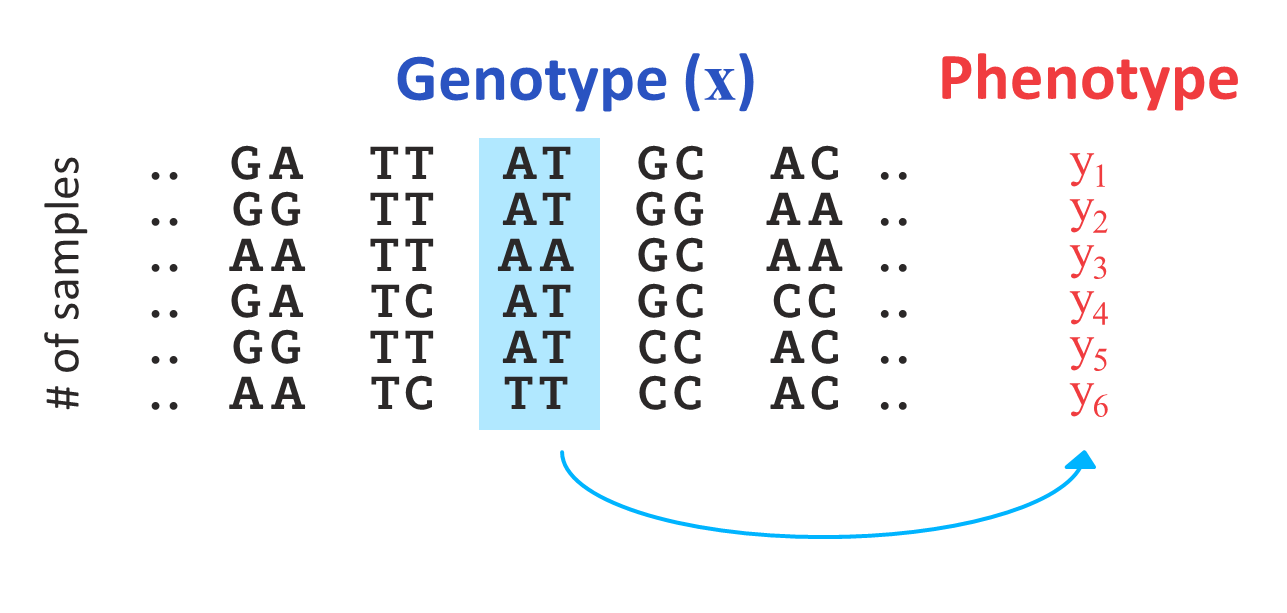
\includegraphics[width=0.6\textwidth]{figures/univariate_model_03.png}\\
%     }
%   }
%   \vskip -1em
%   \begin{align*}
%     \uncover<5->{
%     & y_n = v_{0} + v_{i}x_{ni} + \epsilon, \quad \text{\scriptsize with} \quad \epsilon \sim \mathcal{N} (0, \sigma^2) & \text{\scriptsize Quantitative phenotype} \\[1em]
%     }
%     \uncover<6->{
%     & p\left( y_{n} = 1 | x_{ni}, v_{0}, v_{i} \right)  = \logistic \left( v_{0} + v_{i}x_{ni} \right) & \text{\scriptsize Binary phenotype} \\
%     }
%   \end{align*}
%   \vskip -2em
%   \myfulltwocolumn{0.7}{T}
%   {
%     \uncover<7->{
%     \begin{itemize1}
%       \item Is the coefficient $v_i$ significantly different from 0? $\Rightarrow$ P-values
%     \end{itemize1}
%     }
%   }{
%     \uncover<6->{
%       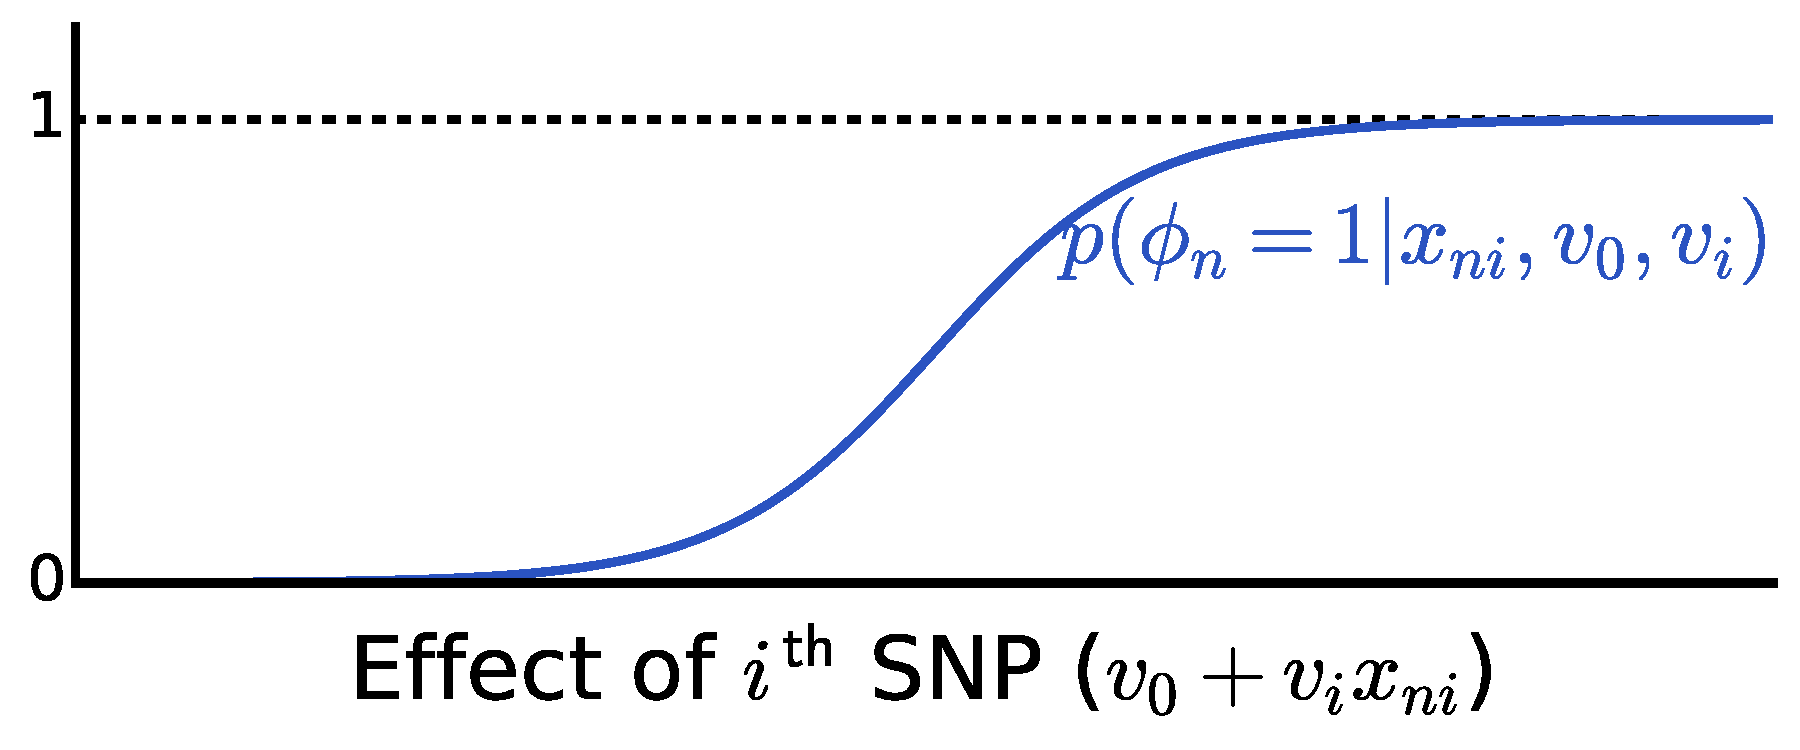
\includegraphics[height=0.13\textheight]{figures/logistic_function_01.pdf}\\
%     }
%   }
% \end{frame}
% 
% \begin{frame}
%   \frametitle{Univariate methods}
%   \vskip -2em
%   \myfulltwocolumn{0.5}{t}
%   {
%     {\center \color{primary}\small \textbf{Strengths}\\} 
%     \vskip 0.5em
%     \uncover<1->{
%     \begin{itemize2}
%       \item Straightforward
%       \item Computationally fast
%       \item Conservative
%       \item Easy to interpret
%     \end{itemize2}
%     }
%   }{
%     \uncover<2->{
%     {\center \color{primary}\small \textbf{Challenges}\\} 
%     \vskip 0.5em
%     \begin{itemize2}
%       %\item SNPs in linkage disequilibrium with the causal $\Rightarrow$ similar significance scores
%       \item Linkage disequilibrium
%       %\item<3-> Concerted mechanism $\Rightarrow$ Small individual effect sizes
%       \item Genetic networks
%       %\item Marginal effect of individual SNPs $\neq$ Combined effects
%       \item Low effect sizes
%     \end{itemize2}
%     }
%   }
%   \uncover<3->
%   {\center
%   \begin{tikzpicture}[node distance=2cm]
%     \node (improve) at ( 0,  0) [origin] {Improvements};
%     \node (multi)   at (-3, -2) [decision] {Multivariate analysis};
%     \node (meta)    at ( 3, -2) [decision] {Meta-analysis};
%     \coordinate (z) at ( 0, -1);
%     \draw [line] (improve) -- (z);
%     \draw [arrow] (z) -| (meta);
%     \draw [arrow] (z) -| (multi);
%   \end{tikzpicture}\\
%   }
% \end{frame}
% 
% \begin{frame}
%   \frametitle{Multivariate methods}
%   {\center
%     \vskip -1em
%     \only<1-1>{
%     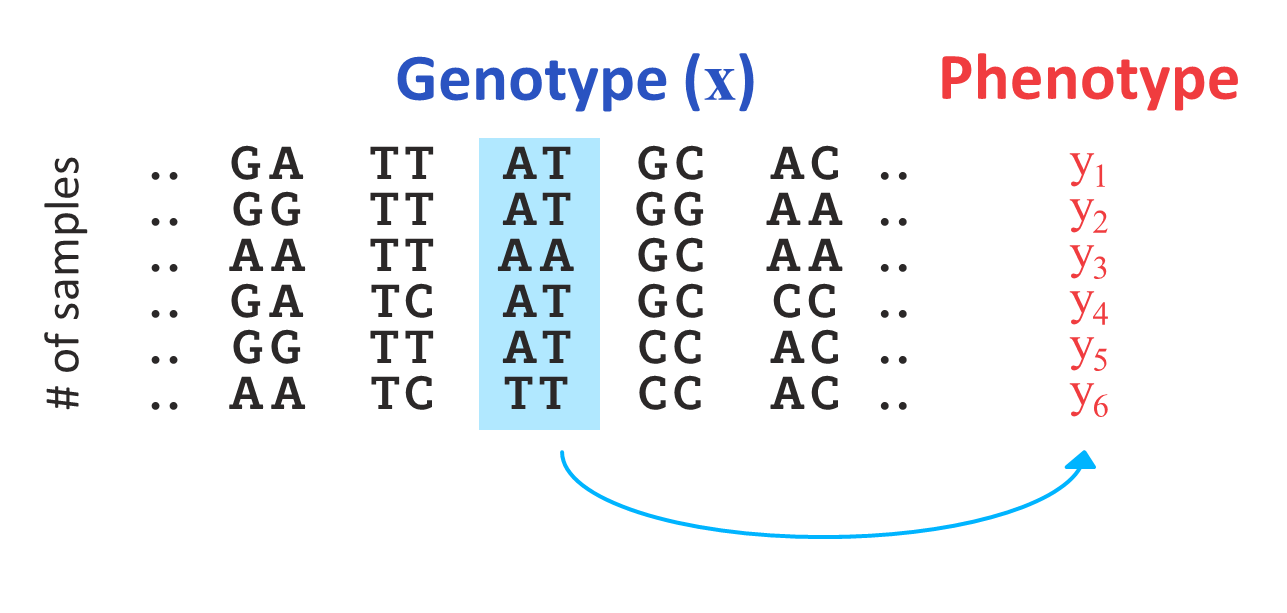
\includegraphics[width=0.6\textwidth]{figures/univariate_model_03.png}\\
%     }
%     \only<2->{
%     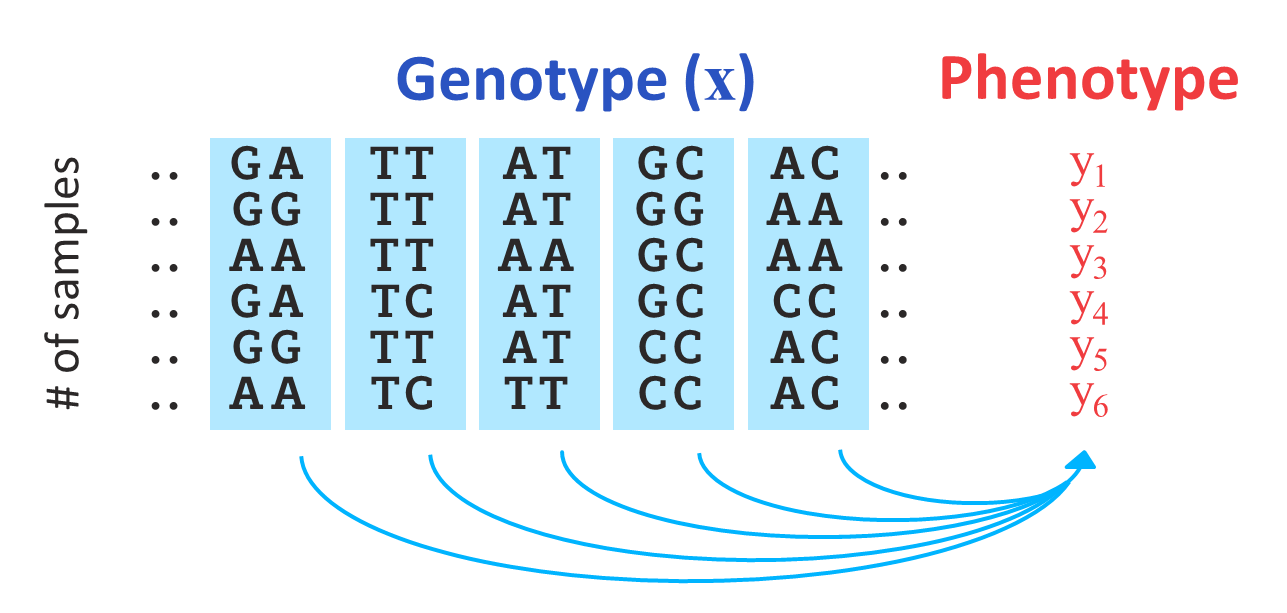
\includegraphics[width=0.6\textwidth]{figures/multivariate_model.png}\\
%     }
%   }
%   \vskip -1em
%   \begin{align*}
%     \uncover<3->{
%     & y_n = v_{0} + \sum_i v_{i}x_{ni} + \epsilon, \quad \text{\scriptsize with} \quad \epsilon \sim \mathcal{N} (0, \sigma^2) & \text{\scriptsize Quantitative phenotype} \\
%     }
%     \uncover<4->{
%     & p\left( y_{n} = 1 | x_{ni}, v_{0}, v_{i} \right)  = \logistic \left( v_{0} + \sum_i v_{i}x_{ni} \right) & \text{\scriptsize Binary phenotype} \\
%     }
%   \end{align*}
%   \vskip -1em
%   \uncover<5->{
%   \begin{itemize1}
%     \item Multivariate methods perform better than univariate methods
%   \end{itemize1}
%   }
% \end{frame}
% 
% %\begin{frame}
% %  \frametitle{Meta-analysis of GWAS}
% %  \begin{itemize1}
% %    \item Small effect sizes $\Rightarrow$ require large sample sizes
% %    \item Combine data from multiple studies to
% %    \begin{itemize1}
% %      \item increase statistical power
% %      \item obtain more precise effect size estimates
% %    \end{itemize1}
% %    \item Use summary statistics from each study, rather than raw data
% %    \item<2-> Current methods generally combine information from univariate analyses
% %    \item<3-> {\color{primary} Can we extract more information from existing data?}
% %  \end{itemize1}
% %\end{frame}
% 
% \begin{frame}
%   \frametitle{Meta-analysis}
%   {\center
%     \vskip -1em
%     \only<1-1>{
%     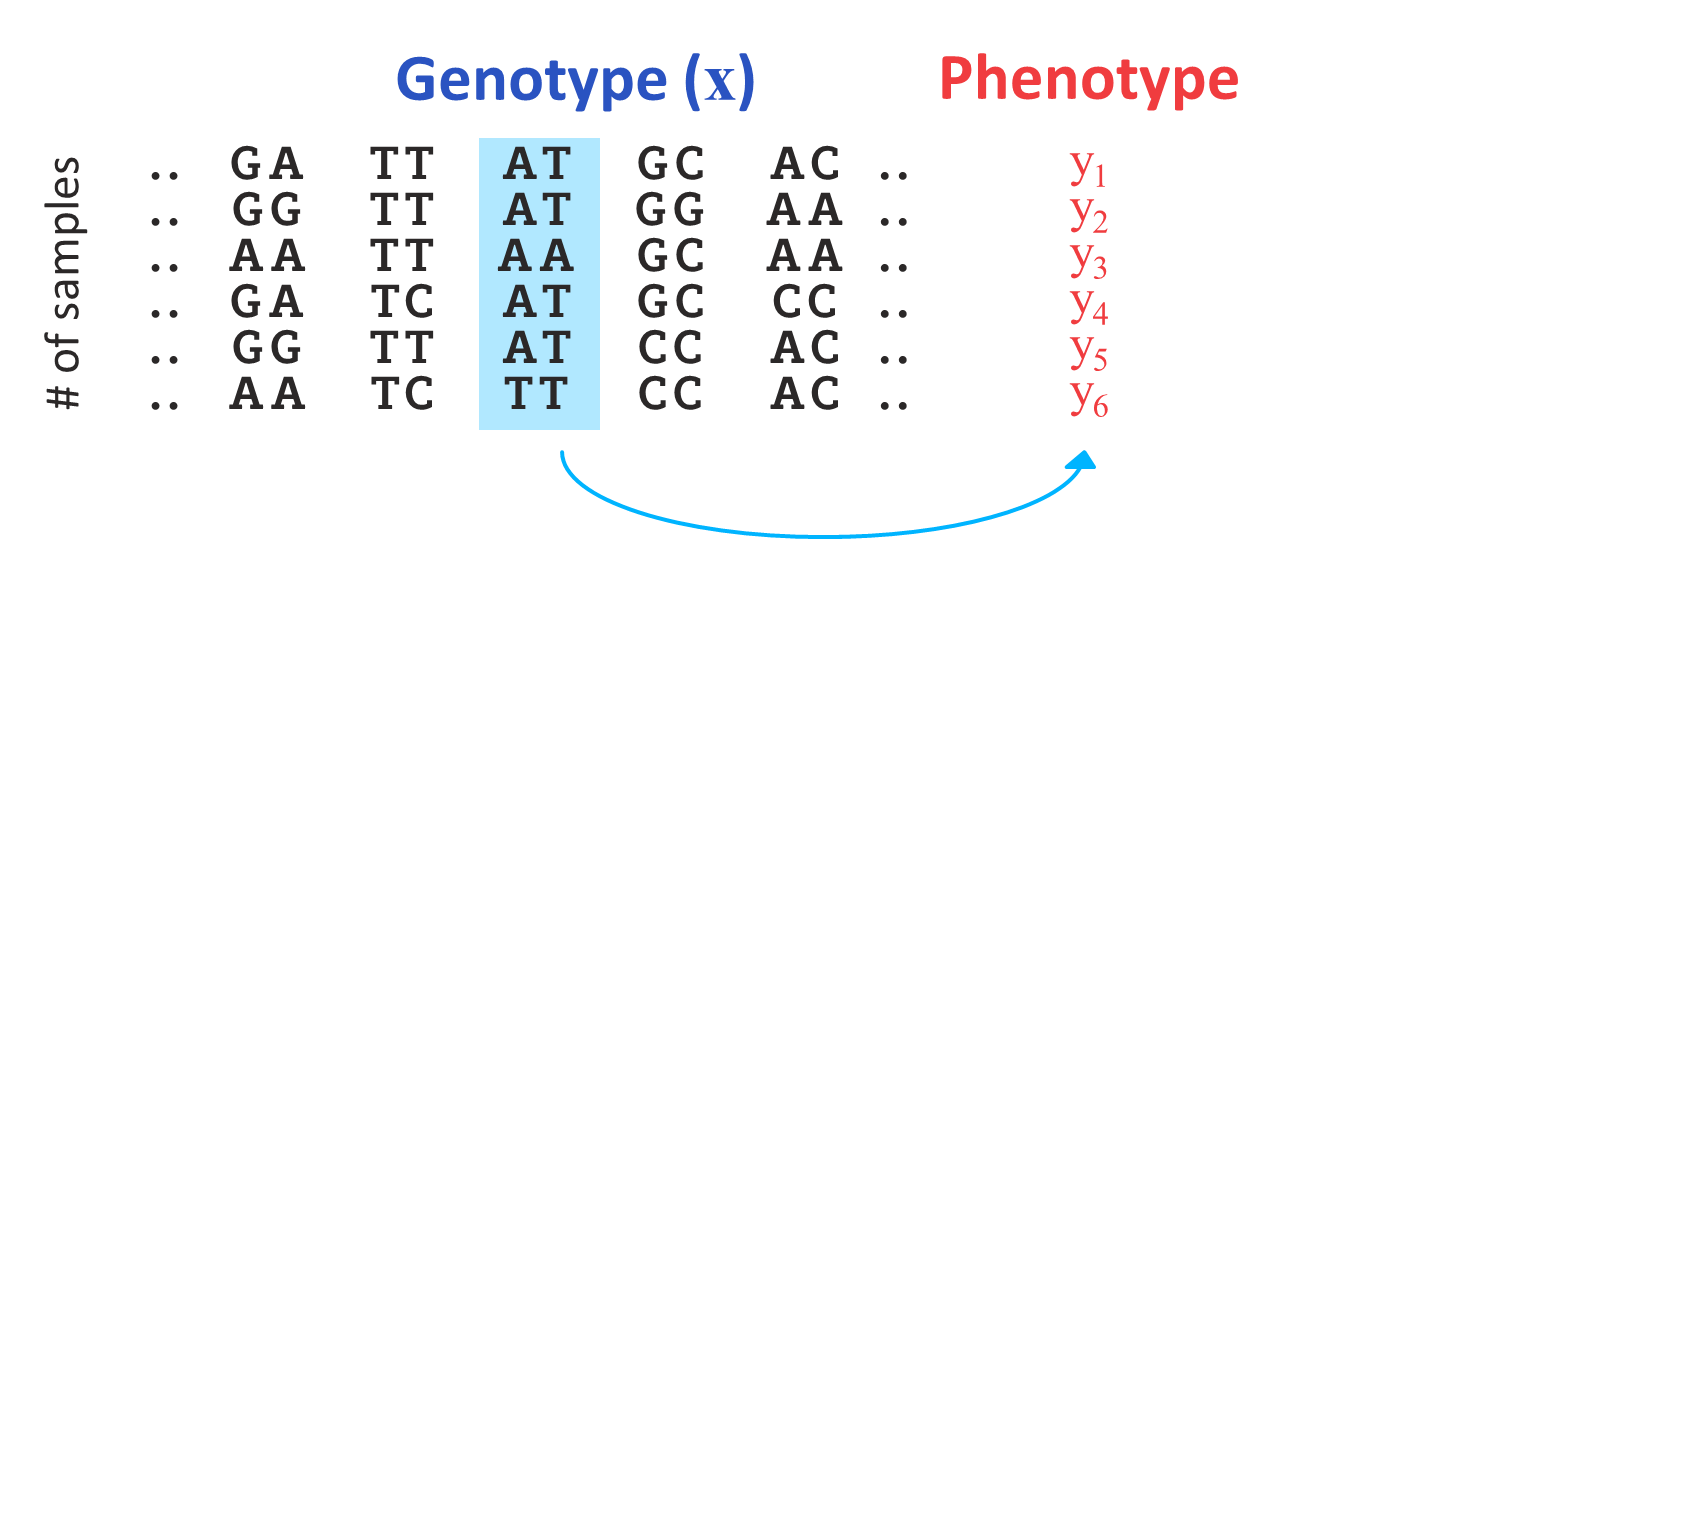
\includegraphics[height=0.9\textheight]{figures/metaanalysis_00.png}\\
%     }
%     \only<2->{
%     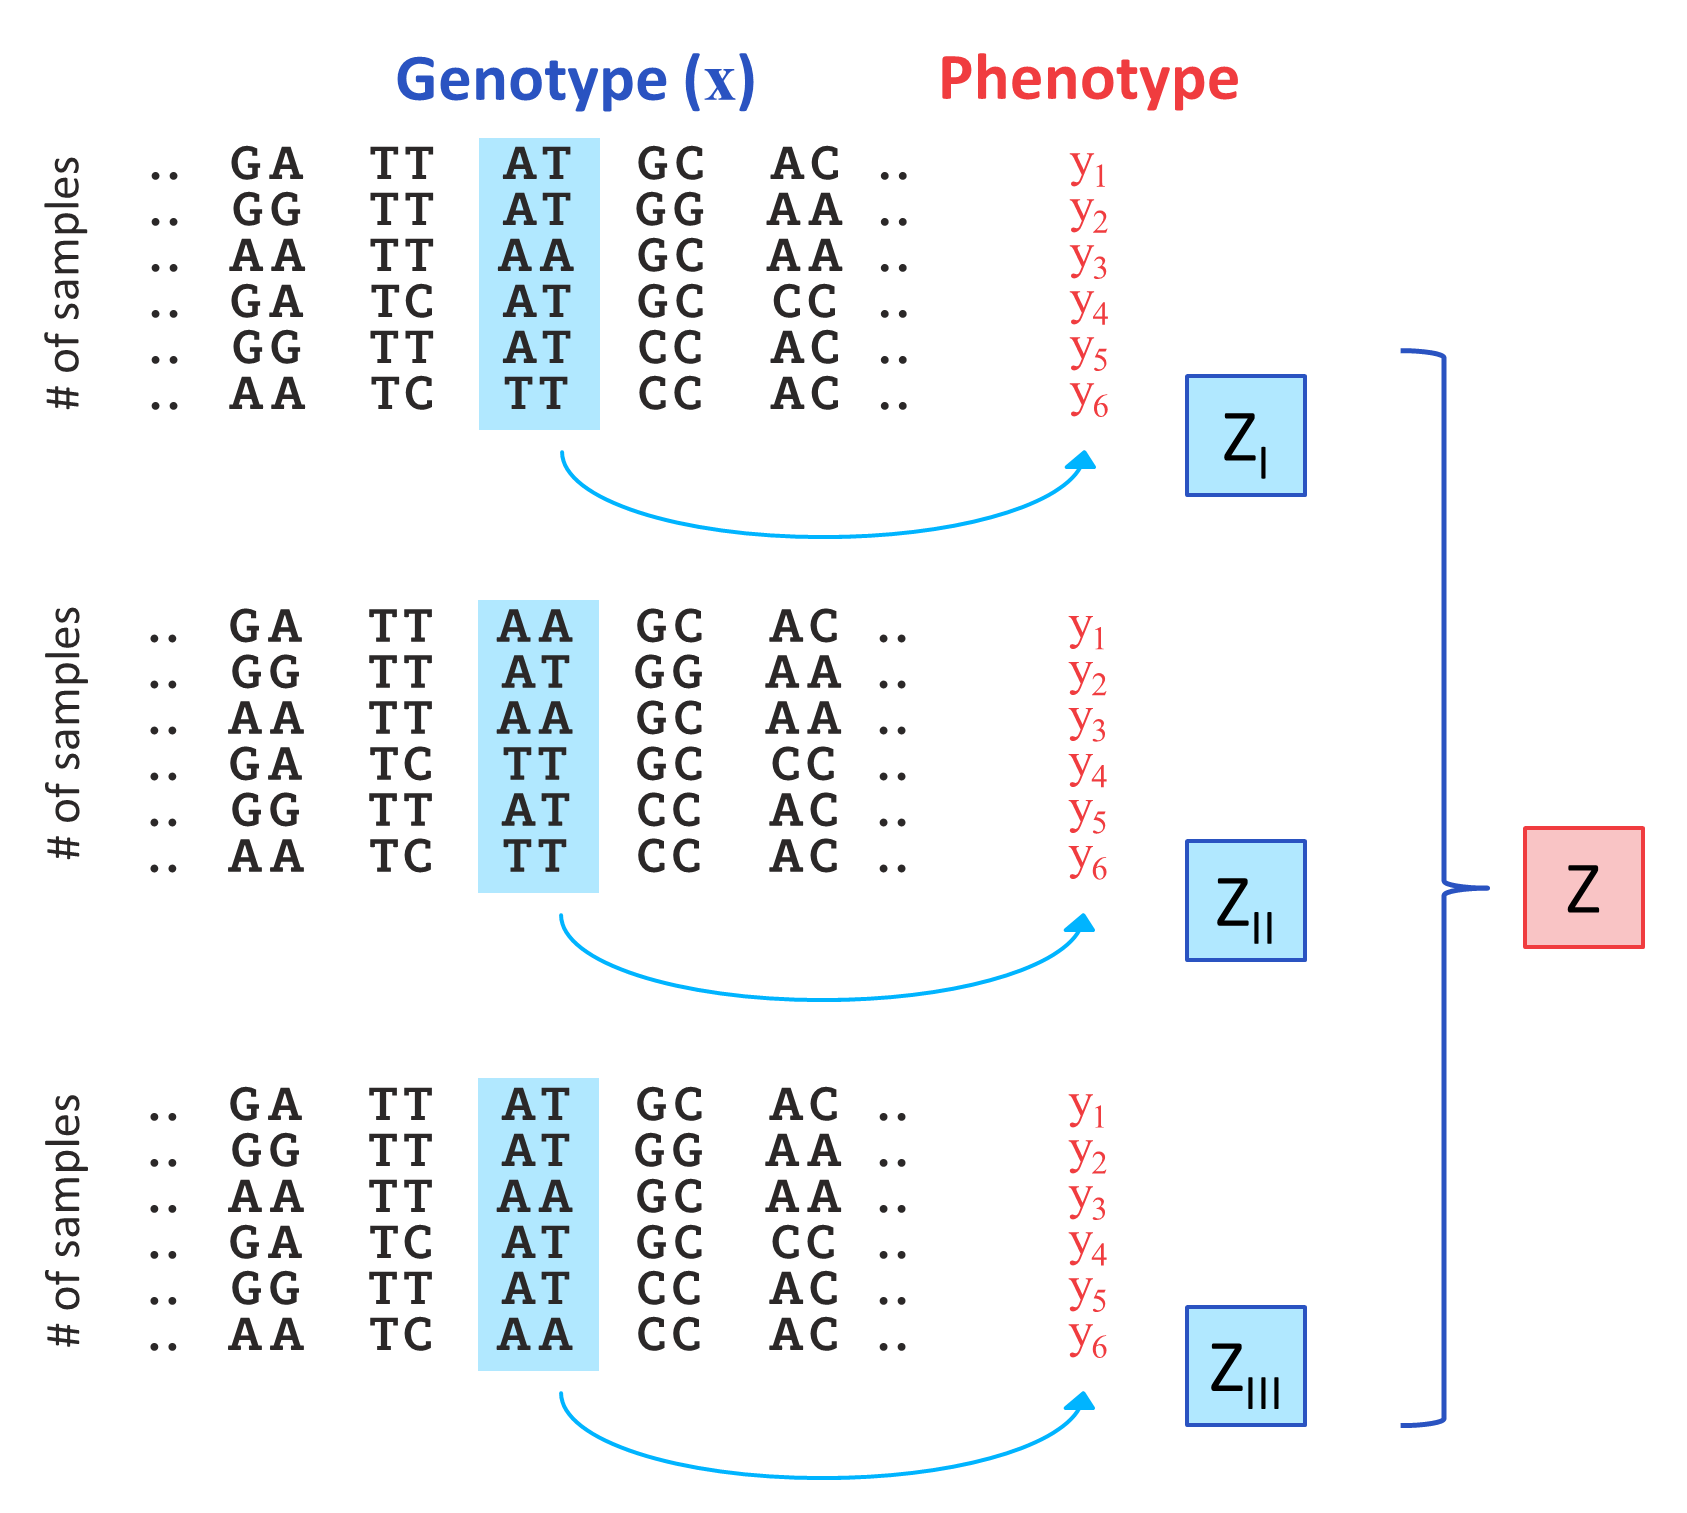
\includegraphics[height=0.9\textheight]{figures/metaanalysis_01.png}\\
%     }
%   }
% \end{frame}
% 
% \begin{frame}
%   \frametitle{Goal of our method}
%   {\center
%     \vskip -1em
%     \only<1-1>{
%     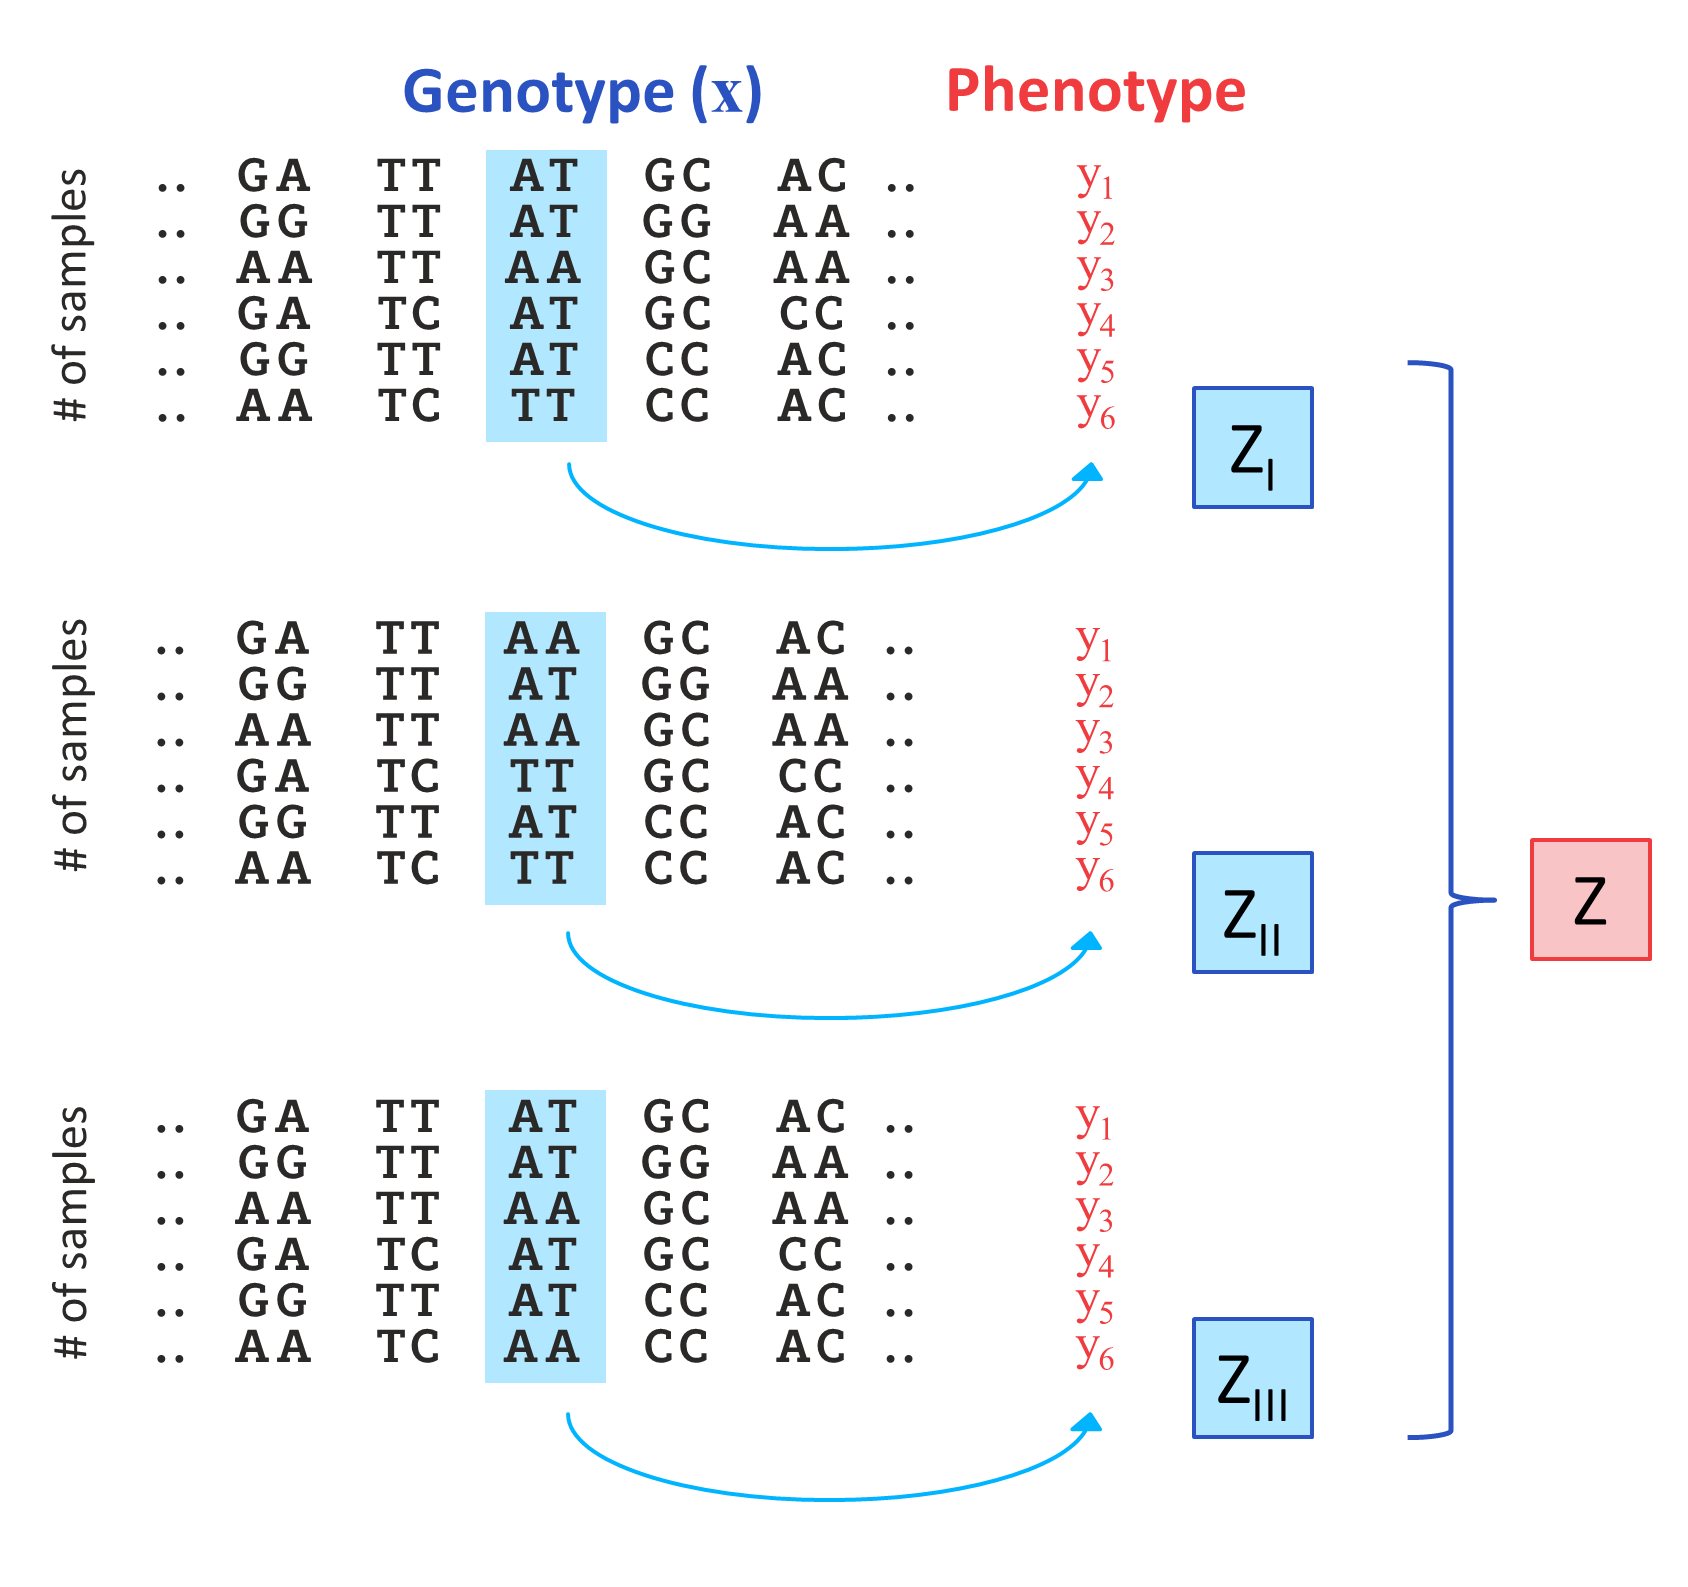
\includegraphics[height=0.9\textheight]{figures/bvslr_00.png}\\
%     }
%     \only<2->{
%     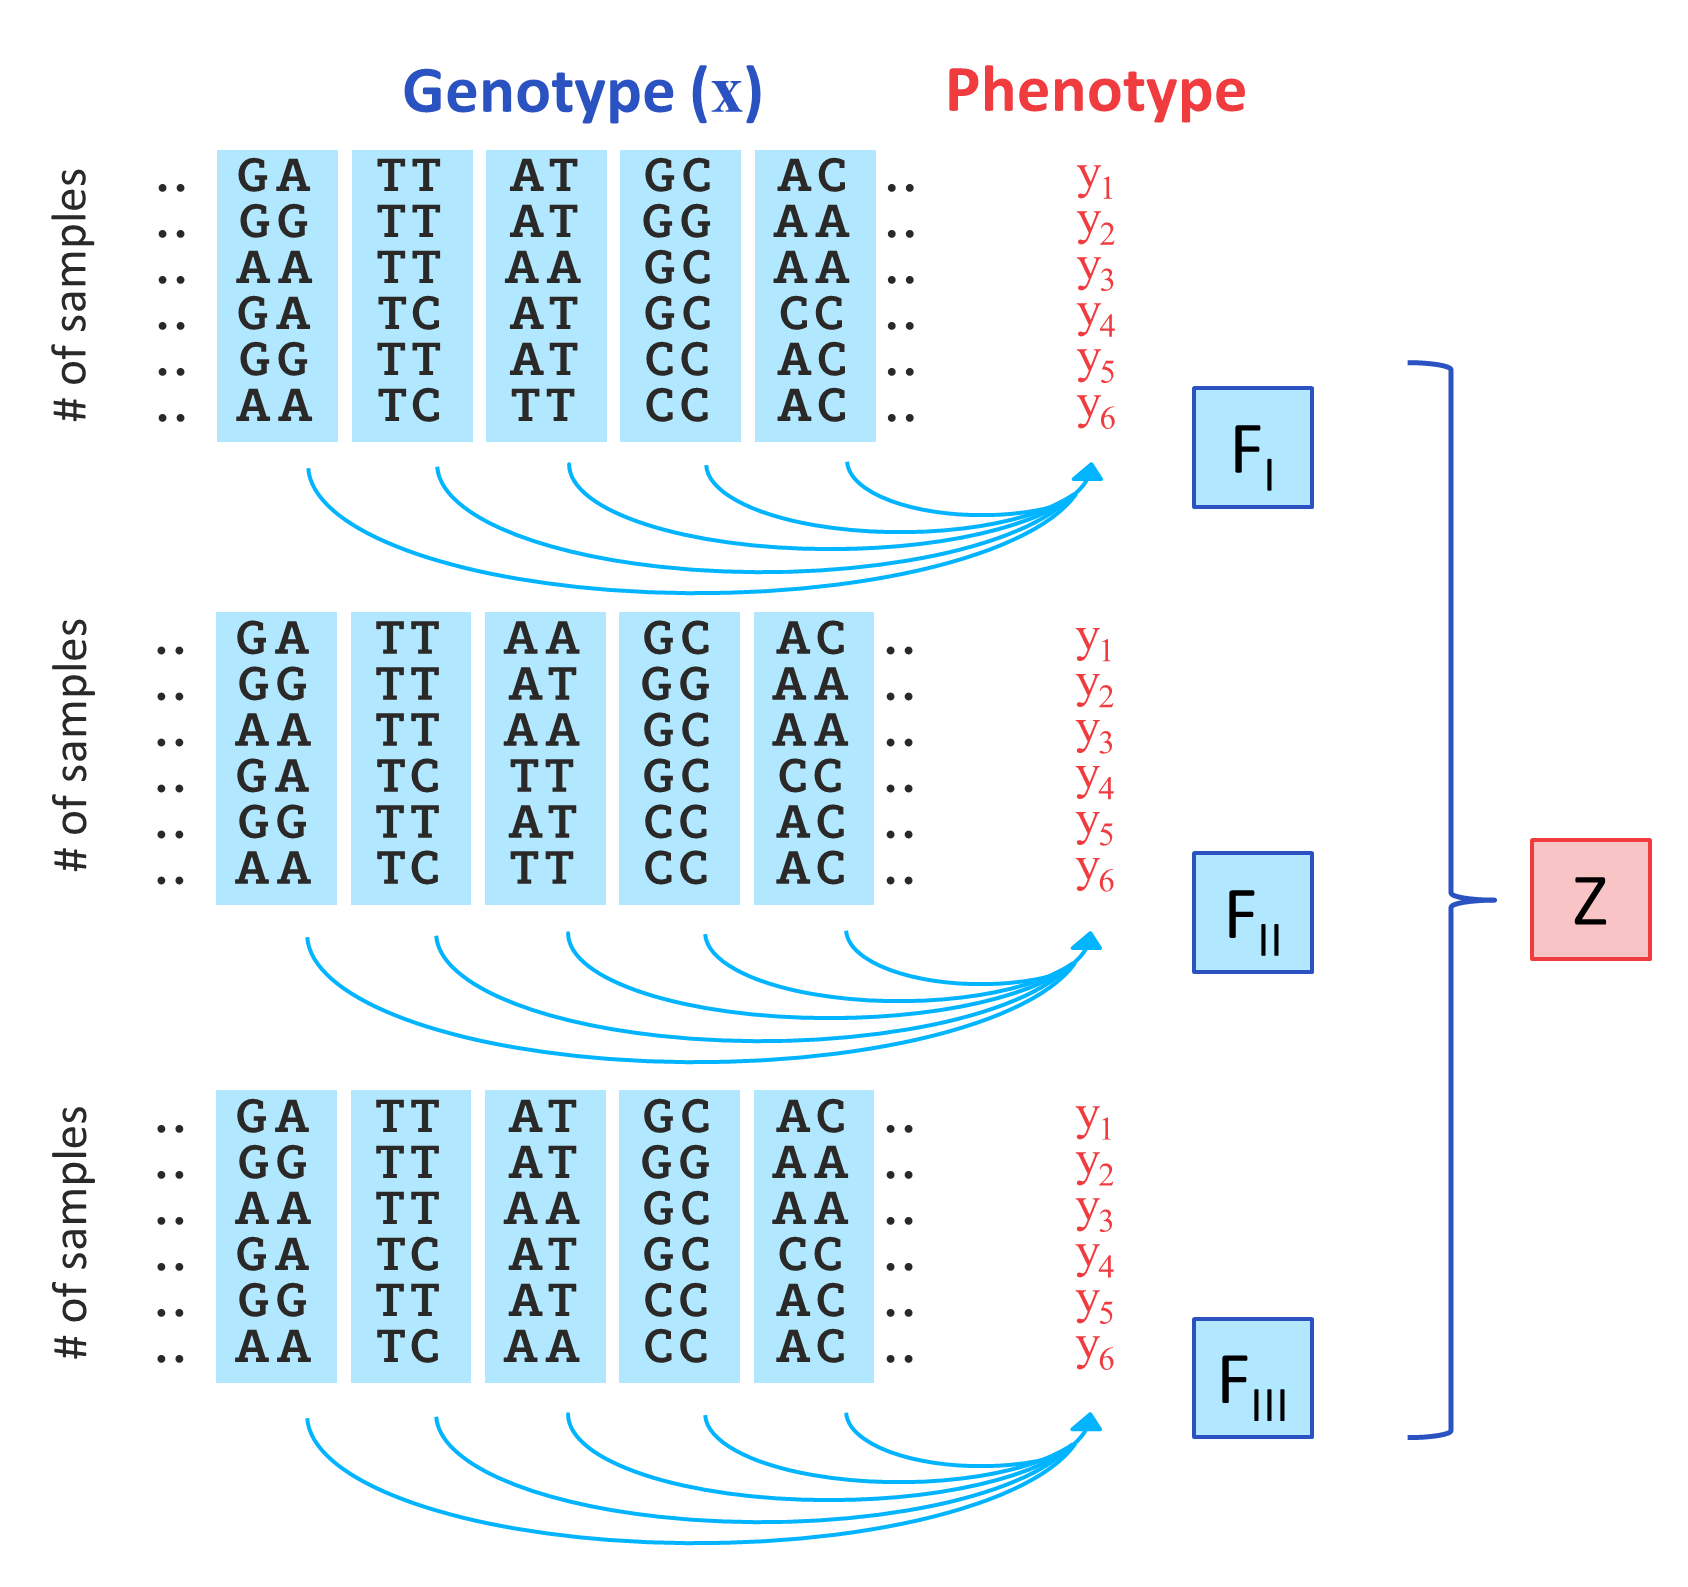
\includegraphics[height=0.9\textheight]{figures/bvslr_01.png}\\
%     %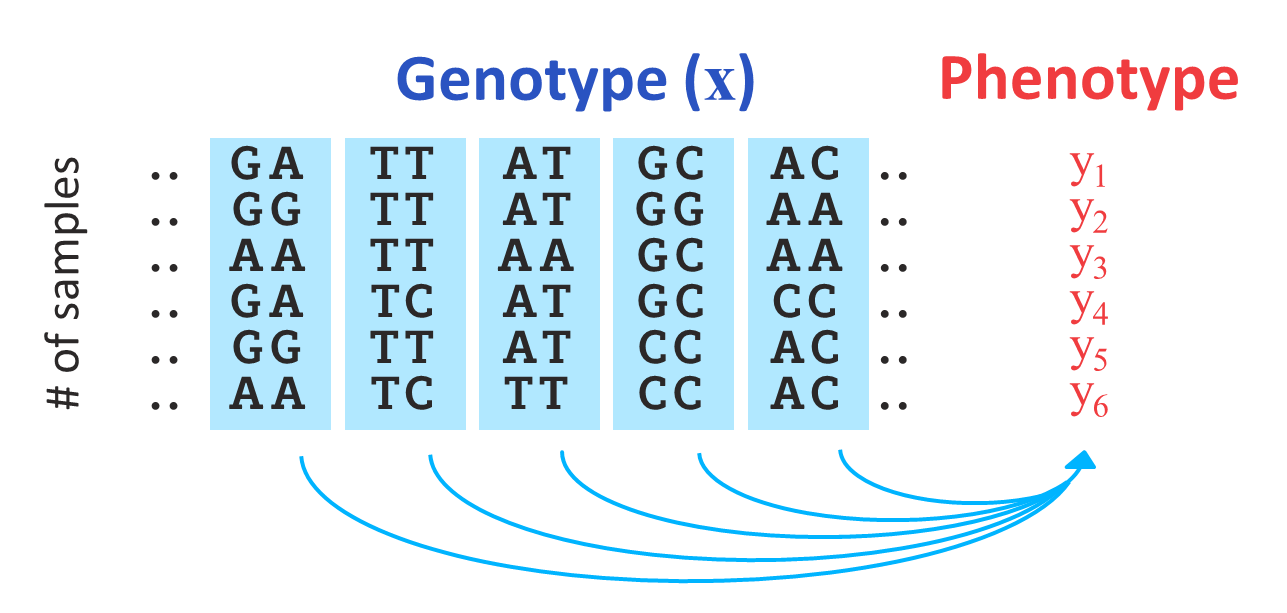
\includegraphics[width=0.6\textwidth]{figures/multivariate_model.png}\\
%     }
%   }
% \end{frame}
% 
% %\begin{frame}
% %  \frametitle{Goal of our method}
% %  {\center
% %  \begin{tikzpicture}[node distance=2cm]
% %    \node (improve) at ( 0,  0) [origin] {GWAS};
% %    \node (multi)   at (-3, -2) [decision] {Multivariate analysis};
% %    \node (meta)    at ( 3, -2) [decision] {Meta-analysis};
% %    \coordinate (z) at ( 0, -1);
% %    \node (q)       at ( 0, -4) [doubt] {?};
% %    \draw [line] (improve) -- (z);
% %    \draw [arrow] (z) -| (meta);
% %    \draw [arrow] (z) -| (multi);
% %    \draw [arrow] (meta) -- (q);
% %    \draw [arrow] (multi) -- (q);
% %  \end{tikzpicture}\\
% %  }
% %  \vskip 1em
% %  \begin{itemize1}
% %    \item Can we extract more information from existing data?
% %  \end{itemize1}
% %\end{frame}
% 
% \begin{frame}
%   \frametitle{Preview of BVSLR}
%   \myfulltwocolumn{0.6}{T}
%   {
%     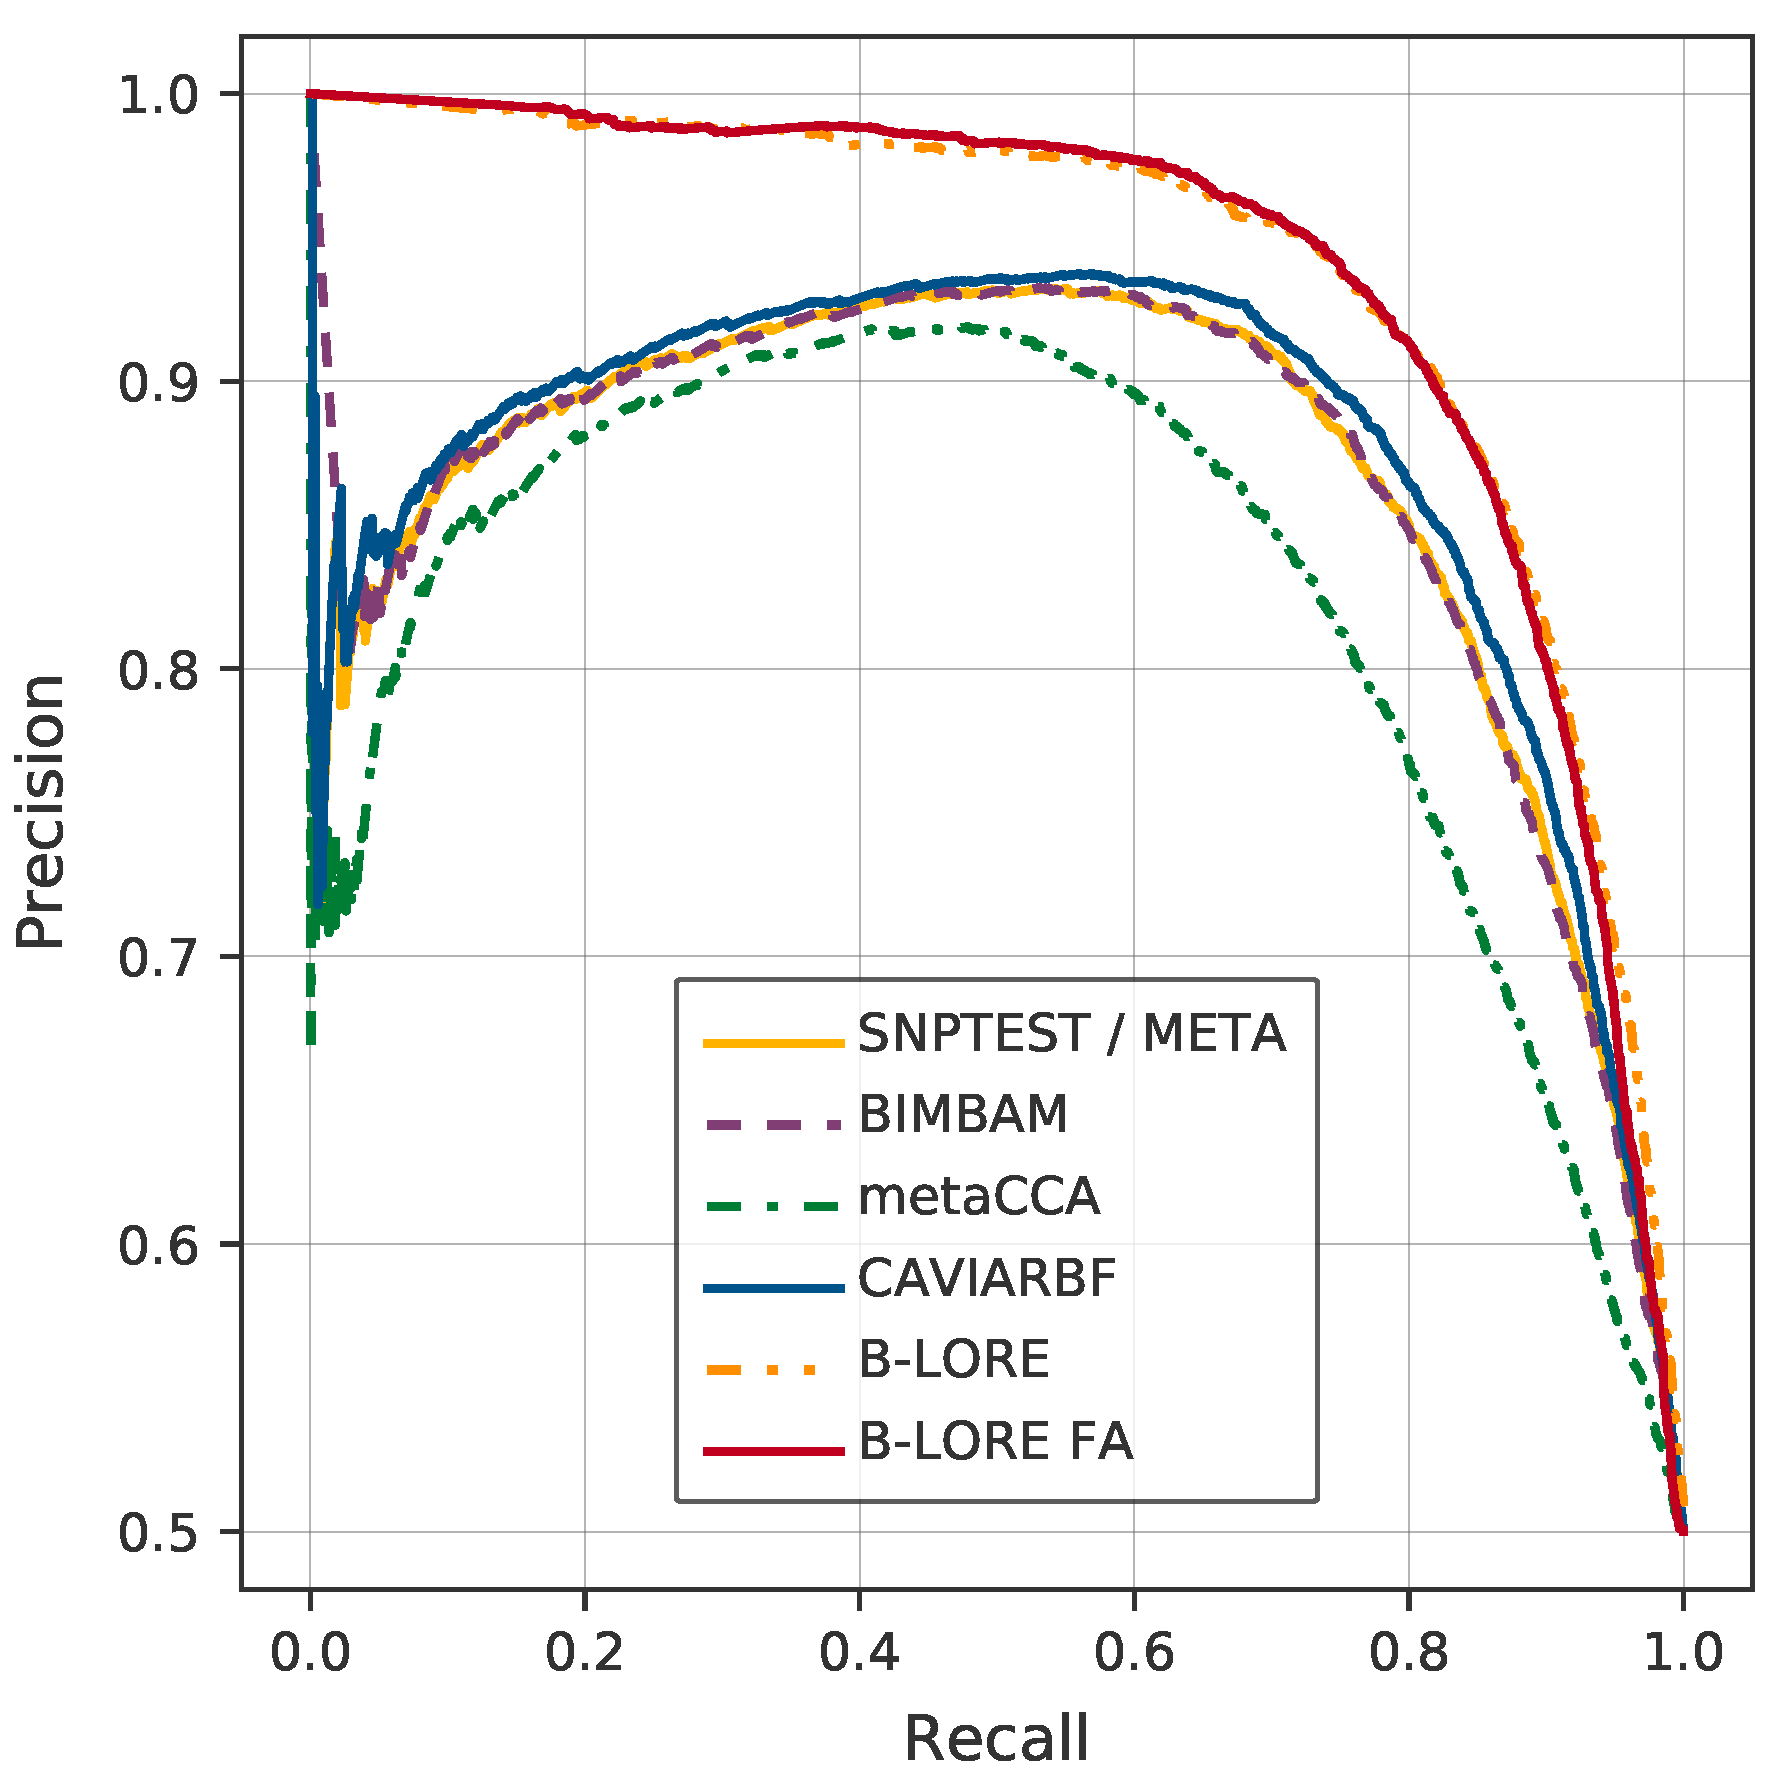
\includegraphics[width=1.0\textwidth]{figures/simu_locus_precision_recall_withld.pdf}\\
%   }{
%     \begin{align*}
%       \text{\scriptsize Precision} & = \frac{\mathrm{TP}}{\mathrm{TP} + \mathrm{FP}} \\
%       \text{\scriptsize Recall}    & = \frac{\mathrm{TP}}{\mathrm{TP} + \mathrm{FN}} \\
%     \end{align*}
%   }
% \end{frame}
% 
% \subsection{Method // Model and inference}
% 
% \begin{frame}
%   \frametitle{Bayesian variable selection regression (BVSR)}
%   \myfulltwocolumn{0.3}{c}
%   {
%     \begin{tikzpicture}
%       \node (a) at (0,0) [highlight] {\textbf{BIMBAM}};
%     \end{tikzpicture}
%   }{
%     Servin and Stephens, \textit{PLoS Genetics} 2007\\
%     Guan and Stephens, \textit{Ann. Appl. Stats.} 2011\\[0.5em]
%   }
%   %Multivariate regression on {\color{primary} \textbf{quantitative}} phenotype $(y)$ :
%   \begin{equation*}
%     y_n = v_{0} + \sum_i v_{i}x_{ni} + \epsilon, \quad \text{\scriptsize with} \quad \epsilon \sim \mathcal{N} (0, \tau^{-1}) \qquad \text{\scriptsize Quantitative phenotype}
%   \end{equation*}
%   \begin{itemize1}
%     \item<2-> Likelihood for $N$ patients:
%           \begin{empheq}[box=\mymathbox]{equation*}
%             p\left(\vy \mid \vx, \vv, \tau \right) = \mathcal{N}\left(\vy \mid \vx^\intercal\vv, \tau^{-1}\idop \right)
%           \end{empheq}
%     \item<3-> Number of SNPs $\gg$ samples $\rightarrow$ {\color{secondary} Overfitting}
%     \item<3-> {\color{primary} Effective priors on $\vv$ for sparsity}
%     %\item MCMC for inference from posterior.
%   \end{itemize1}
% \end{frame}
% 
% %\begin{frame}
% %  \frametitle{BVSR improves SNP identification}
% %  \uncover<1->
% %  {\center
% %    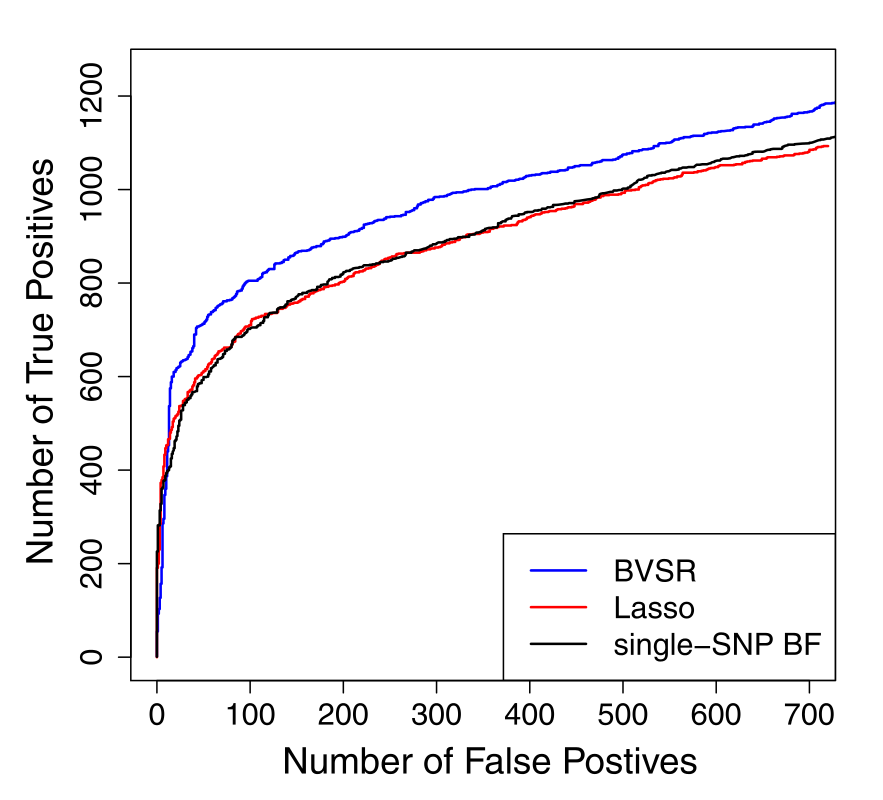
\includegraphics[width=0.5\textwidth]{figures/bvsr_vs_univariate.png}\\[0.7em]
% %  }
% %  \uncover<2>{
% %  \begin{itemize1}
% %    \item {BVSR unfortunately does not allow multivariate metaanalysis}\\[0.5em]
% %    \item {\color{primary} No analytical solution for binary phenotypes}
% %    %\item Future plans
% %  \end{itemize1}
% %  }
% %  \myreference{Guan and Stephens, \textit{Ann. Appl. Stats.} 2011}
% %\end{frame}
% 
% \begin{frame}
%   \frametitle{Bayesian variable selection logistic regression (BVSLR)}
%   \myfulltwocolumn{0.5}{c}
%   {
%     \begin{flalign*}
%       p\left( \phi_{n} = 1 | \vx_{n}, \vv \right)  = \logistic \left( v_{0} + \sum_{i} v_{i}x_{ni} \right) &&\\
%     \end{flalign*}
%   }{
%     \center
%     %\vskip 2em
%     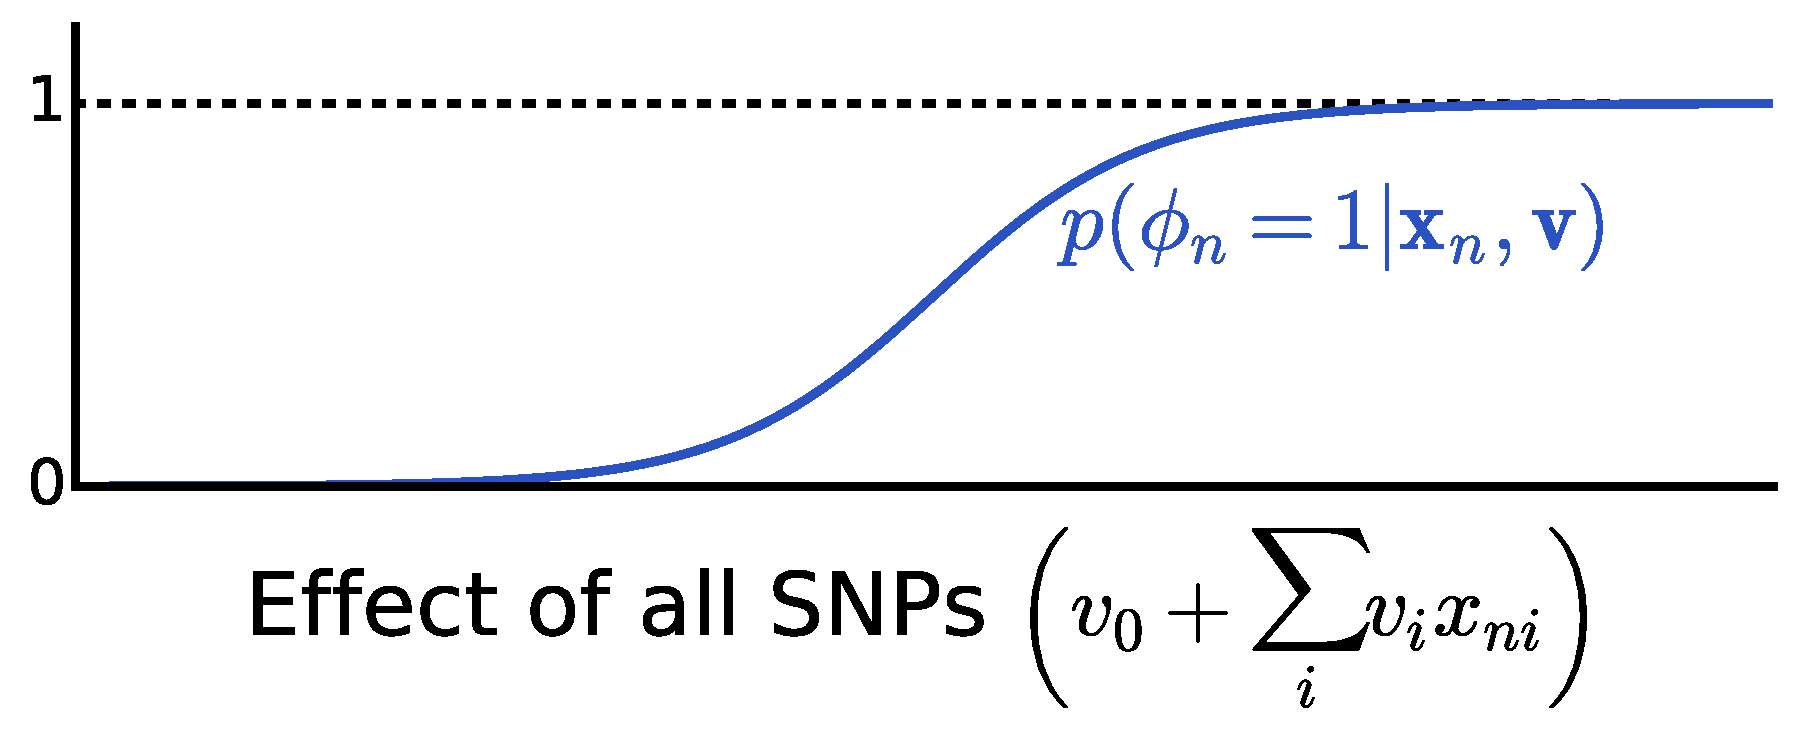
\includegraphics[width=1.0\textwidth]{figures/logistic_function_02.pdf}\\
%   }
%   \begin{itemize1}
%     \item Likelihood for $N$ patients:
%           \begin{empheq}[box=\mymathbox]{equation*}
%             p\left(\bs\phi \mid \vx, \vv \right) = \prod_{n=1}^N p\left(\phi_n | \vx_n, \vv \right) = \prod_{n=1}^N \frac{\exp(\phi_n \vv^\intercal \vx_n )}{1 + \exp( \vv^\intercal \vx_n )}
%           \end{empheq}
%   \end{itemize1}
% \end{frame}
% 
% \begin{frame}
%   \frametitle{LASSO penalisation}
%   %% http://stats.stackexchange.com/questions/177210/why-is-laplace-prior-producing-sparse-solutions/
%   %% http://www.lshtm.ac.uk/library/MSc_MS/2009-10/491467.PDF
%   \myreference{Tibshirani, 1996}
%   \begin{itemize}
%     \item Constraint: $\displaystyle \sum_{i} \left| v_{i} \right| \le t $, where $t (> 0)$ is a \emph{tuning parameter}. \\
%     \item Applied as a Lagrangian penalty to the joint log-likelihood.
%   \end{itemize}
%   \myfulltwocolumn{0.5}{c}
%   {
%     \center
%     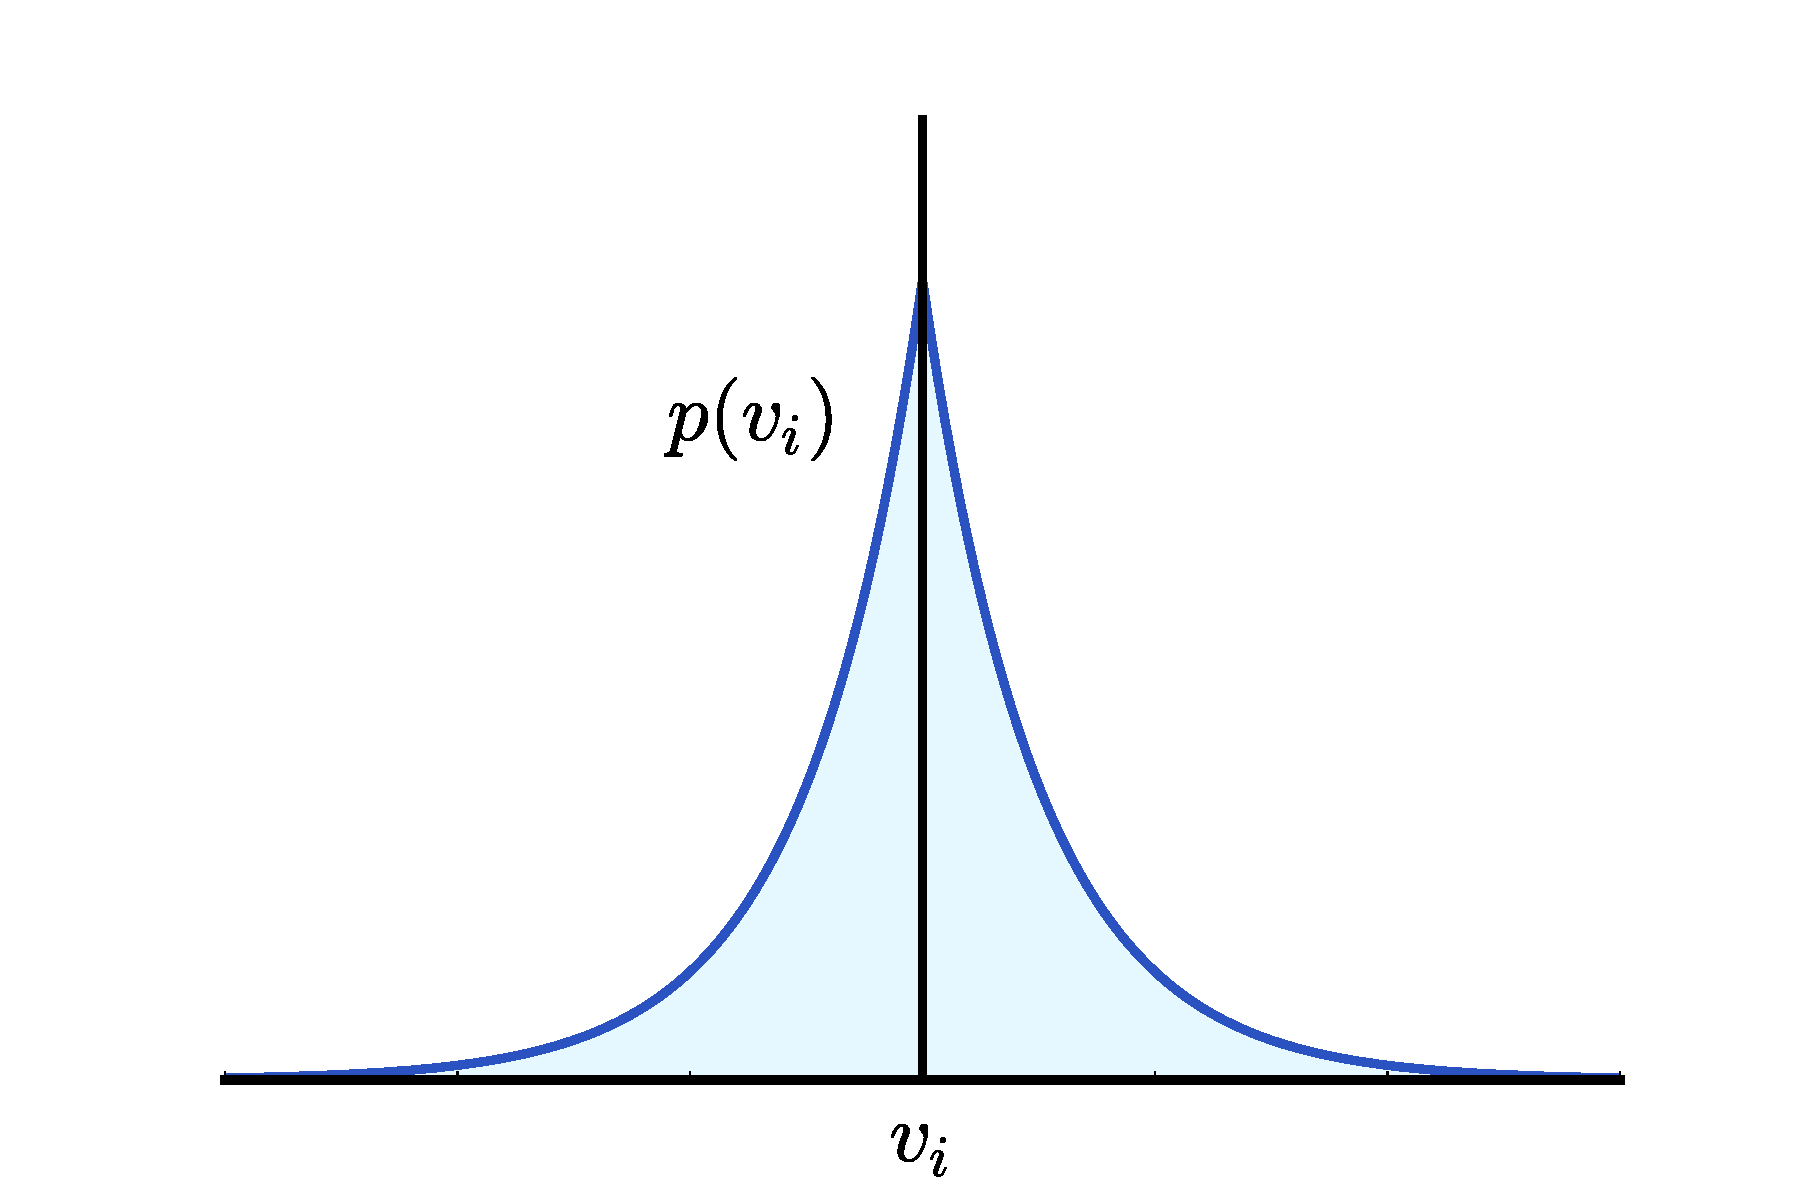
\includegraphics[width=1.0\textwidth]{figures/laplace_prior.pdf}\\
%   }{
%     \begin{infoblock}
%       {LASSO penalty assumes implicit Laplace prior $\rightarrow$ more zero-valued coefficients.}
%     \end{infoblock}
%     {\color{secondary} Problems:}
%     \begin{itemize}
%       \item Multicollinearity
%       \item Variability in penalty parameter
%     \end{itemize}
%   }
% \end{frame}
% 
% \begin{frame}
%   \frametitle{Sparsity in BVSR / BVSLR}
%   Looks at both {\color{primary} null hypothesis} and {\color{secondary}alternate hypothesis}
%   {\center
%     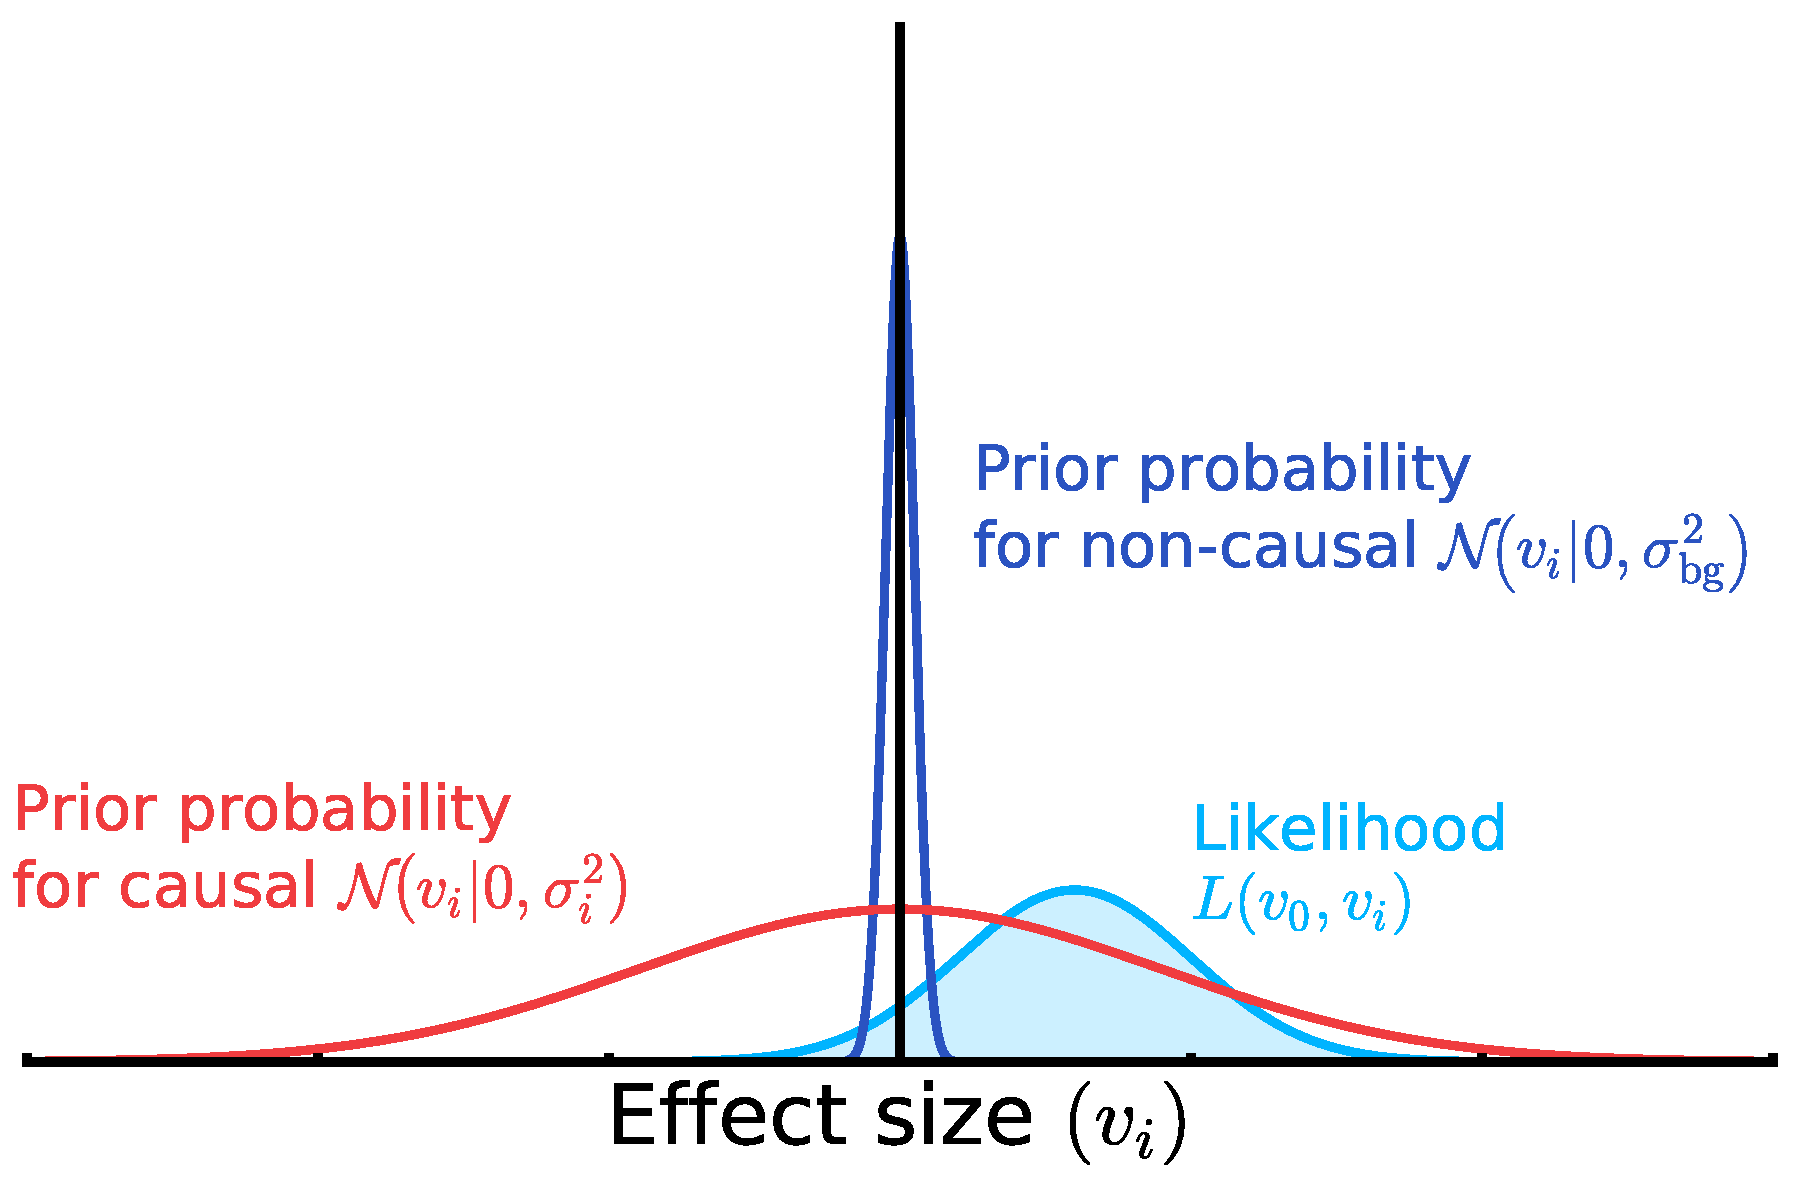
\includegraphics[width=0.8\textwidth]{figures/bayesian_logistic_regression_01.pdf}\\
%   }
% \end{frame}
% 
% \begin{frame}
%   \frametitle{Priors in BVSR}
%   \begin{columns}[c]
%     \begin{column}{0.25\textwidth}
%     \end{column}
%     \begin{column}{0.5\textwidth}
%       \begin{empheq}[box=\mymathbox]{equation*}
%         p\left(\vy \mid \vx, \vv, \tau \right) = \mathcal{N}\left(\vy \mid \vx^\intercal\vv, \tau^{-1}\idop \right)
%       \end{empheq}
%       \begin{flalign*}
%         {\color{subdue} p(\tau) \phantom{\, \, \, \, \, \mid \tau}} &{\color{subdue}= \mathrm{Gamma} \left( \frac{\lambda}{2}, \frac{\kappa}{2} \right)} &\\[0.5em]
%         {\color{subdue} p(v_0 \mid \tau)} &{\color{subdue}= \mathcal{N}\left( v_0 \mid 0, {\sigma_\mu^2}\,/\,{\tau} \right)} &\\[0.5em]
%         p(v_i \mid \tau) &= {\color{primary}\overbrace{(1 - \pi)\,\delta_0}^{\text{Non-causal}}}  \quad + \quad
%                                  {\color{secondary}\underbrace{\pi\,\mathcal{N}\left( v_i \middle\vert {0, {\sigma_a^2}\,/\,{\tau}} \right)}_{\text{Causal}}} &
%       \end{flalign*}
%       \begin{infoblock}{
%         Hyperparameters $\Rightarrow \ \lambda, \kappa, \pi, \sigma_{\!\mu}, \sigma_a$
%       }\end{infoblock}
%     \end{column}
%     \begin{column}{0.25\textwidth}
%     \end{column}
%   \end{columns}
% \end{frame}
% 
% \begin{frame}
%   \frametitle{Priors in BVSLR}
%   \begin{empheq}[box=\mymathbox]{equation*}
%     p\left(\bs\phi \mid \vx, \vv \right) = \prod_{n=1}^N \frac{\exp(\phi_n \vv^\intercal \vx_n )}{1 + \exp( \vv^\intercal \vx_n )}
%   \end{empheq}
%   \vskip 1em
%   \begin{equation*}
%     p\left( v_i \mid \bs\theta \right) =
%           {\color{primary}\overbrace{\left(1 - \pi \right) \mathcal{N}\left(v_i \mid 0, \sigma^2_\text{bg}\right)}^{\text{Non-causal}}} 
%           \quad + \quad
%           {\color{secondary} \underbrace{\pi  \mathcal{N}\left(v_i \mid \mu, \sigma^2 \right)}_{\text{Causal}}}
%   \end{equation*}
%   \vskip 1em
%   \begin{columns}[c]
%     \begin{column}{0.25\textwidth}
%     \end{column}
%     \begin{column}{0.5\textwidth}
%       \begin{infoblock}{
%         Hyperparameters $\bs\theta \Rightarrow \ \pi, \mu, \sigma_\text{bg}, \sigma$
%       }\end{infoblock}
%     \end{column}
%     \begin{column}{0.25\textwidth}
%     \end{column}
%   \end{columns}
% \end{frame}
% 
% \begin{frame}
%   \frametitle{Causality configurations}
%   \vskip -2em
%   \begin{flalign*}
%     p\left( v_i \mid \bs\theta \right) &= 
%                     {\color{primary}\overbrace{\left(1 - \pi \right) \mathcal{N}\left(v_i \mid 0, \sigma^2_\text{bg}\right)}^{\text{Non-causal}}}
%                     \ + \
%                     {\color{secondary} \underbrace{\pi  \mathcal{N}\left(v_i \mid \mu, \sigma^2 \right)}_{\text{Causal}}} \\
%                                        &= 
%                     \sum_{z_i = 0,1} {\color{secondary} \pi^{z_i}} 
%                          {\color{primary} \left(1 - \pi \right)^{(1 - z_i)} }
%                           \mathcal{N}\left( v_i \mid \mu_{\vz,i}, \sigma^2_{\vz,i} \right)
%   \end{flalign*}
%   \begin{equation*}
%     \color{subdue}
%     \mu_{\vz,i} = z_i \mu \text{\quad and \quad}
%     \sigma^2_{\vz,i} = \sigma^2_\text{bg} + z_i \left[\sigma^2 - \sigma^2_\text{bg}  \right]
%   \end{equation*}
% 
%   \begin{columns}[c]
%     \begin{column}{0.2\textwidth}
%       {
%       }
%     \end{column}
%     \begin{column}{0.6\textwidth}
%       {
%         \begin{infoblock}{
%         $\vz \in \{0, 1\}^I \Rightarrow$ Causality configurations
%         \vskip 0.5em
%         \begin{itemize1}
%           \item $z_i = 1$ \qquad SNP $i$ is causal
%           \item $z_i = 0$ \qquad SNP $i$ is non-causal
%         \end{itemize1}
%         }\end{infoblock}
%       }
%     \end{column}
%     \begin{column}{0.2\textwidth}
%       {
%       }
%     \end{column}
%   \end{columns}
% 
% \end{frame}
% 
% \begin{frame}
%   \frametitle{Optimising the hyperparameters}
%   \only<1-2>{
%   \begin{equation*}
%     p\left( v_i \mid \bs\theta \right) = \sum_{z_i = 0,1} \pi^{z_i} \left(1 - \pi \right)^{(1 - z_i)} \mathcal{N}\left( v_i \mid \mu_{\vz,i}, \sigma^2_{\vz,i} \right)
%   \end{equation*}
%   \vskip 1em
%   }
%   \only<2-2>{
%   \begin{equation*}
%     p\left( \vv \mid \bs\theta \right) = \sum_{\vz} p\left( \vz \mid \bs\theta \right) \mathcal{N}\left( \vv \mid \bs\mu_\vz, \diag(\bs\sigma^2_\vz) \right)
%   \end{equation*}
%   }
%   \uncover<3->{
%   \begin{equation*}
%     {\color{sub1} p\left( \vv \mid \bs\theta \right)} = \sum_{\vz} p\left( \vz \mid \bs\theta \right) \mathcal{N}\left( \vv \mid \bs\mu_\vz, \diag(\bs\sigma^2_\vz) \right)
%   \end{equation*}
%   }
%   \uncover<4->{
%   \begin{equation*}
%     {\color{sub2} p\left(\bs\phi \mid \vx, \vv \right)} = \prod_{n=1}^N \frac{\exp(\phi_n \vv^\intercal \vx_n )}{1 + \exp( \vv^\intercal \vx_n )}
%   \end{equation*}
%   \vskip 1em
%   }
%   \uncover<5->{
%   \emph{Evidence approximation}: Maximising the marginal likelihood
%   \begin{flalign*}
%     mL(\bs\theta) & = p \left( \bs\phi \mid \vx, \bs\theta \right) & \\
%                   & = \int {\color{sub2} p \left( \bs\phi \mid \vx, \vv \right)}
%                            {\color{sub1} p \left( \vv \mid \bs\theta \right)} 
%                            d\vv \rightarrow \max & \\
%     mL(\bs\theta) &= \sum_{\vz} {\color{sub1} p\left( \vz \mid \bs\theta \right)}
%                      \int {\color{sub2} p \left( \bs\phi \mid \vx, \vv \right)}
%                           {\color{sub1} \mathcal{N}\left( \vv \mid \bs\mu_\vz, \diag(\bs\sigma^2_\vz) \right)}
%                           d\vv &
%   \end{flalign*}
%   }
%   {\center
%     \vskip -2em
%     \hspace{0.1mm} \only<1-5>{\phantom{Laplace approximation (?)}}\only<6-6>{Laplace approximation (?)}\only<7->{\st{Laplace approximation (?)}}\\
%   }
% \end{frame}
% 
% \begin{frame}
%   \frametitle{Quasi-Laplace approximation}
%   \begin{flalign*}
%     \color{normal text.fg!15!normal text.bg}
%     &mL(\bs\theta) = \sum_{\vz} {\color{sub1} p\left( \vz \mid \bs\theta \right)}
%                      \int {\color{sub2} p \left( \bs\phi \mid \vx, \vv \right)}
%                           {\color{sub1} \mathcal{N}\left( \vv \mid \bs\mu_\vz, \diag(\bs\sigma^2_\vz) \right)}
%                           d\vv &\\[0.5em]
%     & {\color{sub2} p\left( \bs\phi \mid \vx, \vv \right)} {\color{sub1} \mathcal{N}\left( \vv \mid \bs\mu_\vz, \diag(\bs\sigma^2_\vz) \right)} &\\
%     & \only<1-1>{
%        \qquad \qquad =
%        {\color{light} \underbrace{ {\color{sub2} p\left( \bs\phi \mid \vx, \vv \right)} {\color{black} \mathcal{N}\left(\vv \mid \tilde{\bs\mu}, \diag(\tilde{\bs\sigma}^{2}) \right)} }_{
%                        \displaystyle \propto \mathcal{N} \left( \mathbf{v} \mid \tilde{\vv}, \tilde{\bs\Lambda}^{-1} \right)}
%        }
%       \times \frac{{\color{sub1}\mathcal{N}\left( \vv \mid \bs\mu_\vz, \diag(\bs\sigma^2_\vz) \right)}}{\color{black} \mathcal{N}\left(\vv \mid \tilde{\bs\mu}, \diag(\tilde{\bs\sigma}^{2}) \right) }
%      } 
%      \only<2->{
%        \qquad \qquad =
%        {\color{black} \underbrace{ {\color{sub2} p\left( \bs\phi \mid \vx, \vv \right)} {\color{black} \mathcal{N}\left(\vv \mid \tilde{\bs\mu}, \diag(\tilde{\bs\sigma}^{2}) \right)} }_{
%                        \displaystyle \propto \mathcal{N} \left( \mathbf{v} \mid \tilde{\vv}, \tilde{\bs\Lambda}^{-1} \right)}
%        }
%       \times \frac{{\color{sub1}\mathcal{N}\left( \vv \mid \bs\mu_\vz, \diag(\bs\sigma^2_\vz) \right)}}{\color{black} \mathcal{N}\left(\vv \mid \tilde{\bs\mu}, \diag(\tilde{\bs\sigma}^{2}) \right) }
%      }
%    &
%   \end{flalign*}
% \end{frame}
% 
% \begin{frame}
%   \frametitle{Analytical solution}
%   \begin{flalign*}
%     mL(\bs\theta) & = p \left( \bs\phi \mid \vx, \bs\theta \right) & \\
%                   & \approx D'  \sum_{\vz} p(\vz \mid \bs\theta)
%                                 \frac{\left| \diag(\bs\lambda_\vz ) \right|^{\frac{1}{2}}}{\left| \bs\Lambda_\vz \right|^{\frac{1}{2}}}
%                                 \exp\left( -\frac{1}{2}  \bs\mu_\vz^\intercal \diag(\bs\lambda_\vz) \bs\mu_\vz + \frac{1}{2} \vv_\vz^\intercal \bs\Lambda_\vz \vv_\vz \right) &\\
%     \text{where} &&\\
%     \bs\Lambda_\vz  &:=  \tilde{\bs\Lambda} -  \diag(\tilde{\bs\lambda}) + \diag(\bs\lambda_\vz) &\\
%     \vv_\vz          &:=  \bs\Lambda_\vz^{-1} \left[ \tilde{\bs\Lambda}\tilde{\vv} + \diag(\bs\lambda_\vz)\bs\mu_\vz  - \diag(\tilde{\bs\lambda})\tilde{\bs\mu} \right] &
%   \end{flalign*}
%   \begin{itemize1}
%     \item Optimization can be done by gradient descent methods (\eg L-BFGS).
%   \end{itemize1}
% \end{frame}
% 
% \begin{frame}
%   \frametitle{Inference of causality in BVSLR}
%   Using the definition of conditional probability,
%   \begin{equation*}
%     p(\vz \mid \bs\phi, \vx, \bs\theta) = \frac{p(\bs\phi, \vz \mid \vx, \bs\theta)}
%                                                         {p(\bs\phi \mid \vx, \bs\theta)}
%   \end{equation*}
%   The posterior probability for SNP $i$ to be causal is
%   \begin{empheq}[box=\mymathbox]{equation*}
%     p(z_i = 1 \mid \bs\phi, \vx, \theta) = \sum_{\vz: z_i=1} p(\vz \mid \bs\phi, \vx, \bs\theta)
%   \end{empheq}
%   \uncover<2>{
%   The probability for a locus to be causal $=$ 1 $-$ probability of \emph{not} having a single causal SNP
%   \begin{empheq}[box=\mymathbox]{equation*}
%     p\left(\text{locus is causal} \mid \bs\phi, \vx, \bs\theta\right) = 1 - p\left(\vz  = \bs 0 \mid \bs\phi, \vx, \bs\theta\right)
%   \end{empheq}
%   }
% \end{frame}
% 
% \begin{frame}
%   \frametitle{BVSLR can be extended to multiple studies}
%   \begin{align*}
%     mL(\bs\theta) & = p \left( \bs\phi \mid \vx_1, \vx_2, \ldots , \vx_S, \bs\theta \right) \\
%                   & = \int p \left( \bs\phi \mid \vx_1, \vx_2, \ldots , \vx_S, \vv \right) p \left( \vv \mid \bs\theta \right) d\vv \rightarrow \max \\
%   \end{align*}
%   Assuming the quasi-Laplace approximation holds for each study,
%   {\color{primary}
%   \begin{align*}
%     \prod_{s=1}^{S} \left[ p \left( \bs\phi \mid \vx_s, \vv \right) \mathcal{N} \left( \mathbf{v} \mid \tilde{\bs\mu}_{\vz,s}, \diag(\tilde{\bs\sigma}_{\vz,s}^2) \right) \right]
%         & \propto \prod_{s=1}^{S} \mathcal{N} \left( \vv \mid \tilde{\vv}_s, \tilde{\bs\Lambda}_s^{-1} \right) \\
%         & = \mathcal{N} \left( \vv \mid \tilde{\vv}, \tilde{\bs\Lambda}^{-1} \right)
%   \end{align*}
%   }
%   where $\displaystyle \tilde{\bs\Lambda} = \sum_{s=1}^{S} \tilde{\bs\Lambda}_s$ and $\displaystyle \tilde{\vv} = \tilde{\bs\Lambda}^{-1} \sum_{s=1}^{S} \tilde{\bs\Lambda}_s \tilde{\vv}_s$
% \end{frame}
% 
% %\begin{frame}
% %  \frametitle{Expectations from BVSLR}
% %  \begin{itemize1}
% %    \item Multivariate analyses takes account of strong local genetic correlation of SNPs (linkage disequilibrium).
% %    \item Analysis from ``summary statistics'' of multiple GWAS cohorts.
% %    \item {\color{primary}We integrate out the SNP effect sizes with their unavoidably large estimation errors, for robust evaluation of hyperparameters}.
% %    \item Thus, we expect BVSLR to extract more information from signals that exist in GWAS data (in much the same way as BVSR / BIMBAM benefits over classical methods in single cohorts). 
% %  \end{itemize1}
% %\end{frame}
% 
\subsection{Results // metaanalysis simulation}

\begin{frame}
  \frametitle{Simulation details}
  \begin{itemize}
    \setlength{\parskip}{4pt}
    \item Genotype: German Myocardial Infarction Family Study (GERMIFS)
    \item Five cohorts {\color{hidden}: G1, G2, G3, G4, G5}
    \item Phenotype simulation:
    \begin{eqnarray*}
      \text{Disease liability \quad} \color{primary} Y_{n}  =  \color{primary} \sum_{i} v_{i}x_{ni} + \varepsilon_{n} \\      
      \Var\left( \sum_{i} v_{i}x_{ni} \right) = h_g^2 = 0.4 \text{ and } \Var(\varepsilon) = 0.6
    \end{eqnarray*}
    Cases are sampled from $Y_n$ exceeding the threshold of normal distribution truncating the proportion of $k$ (disease prevalence)
  \end{itemize}
\end{frame}

\begin{frame}
  \frametitle{Simulation details}
  \myfulltwocolumn{0.7}{b}
  {
    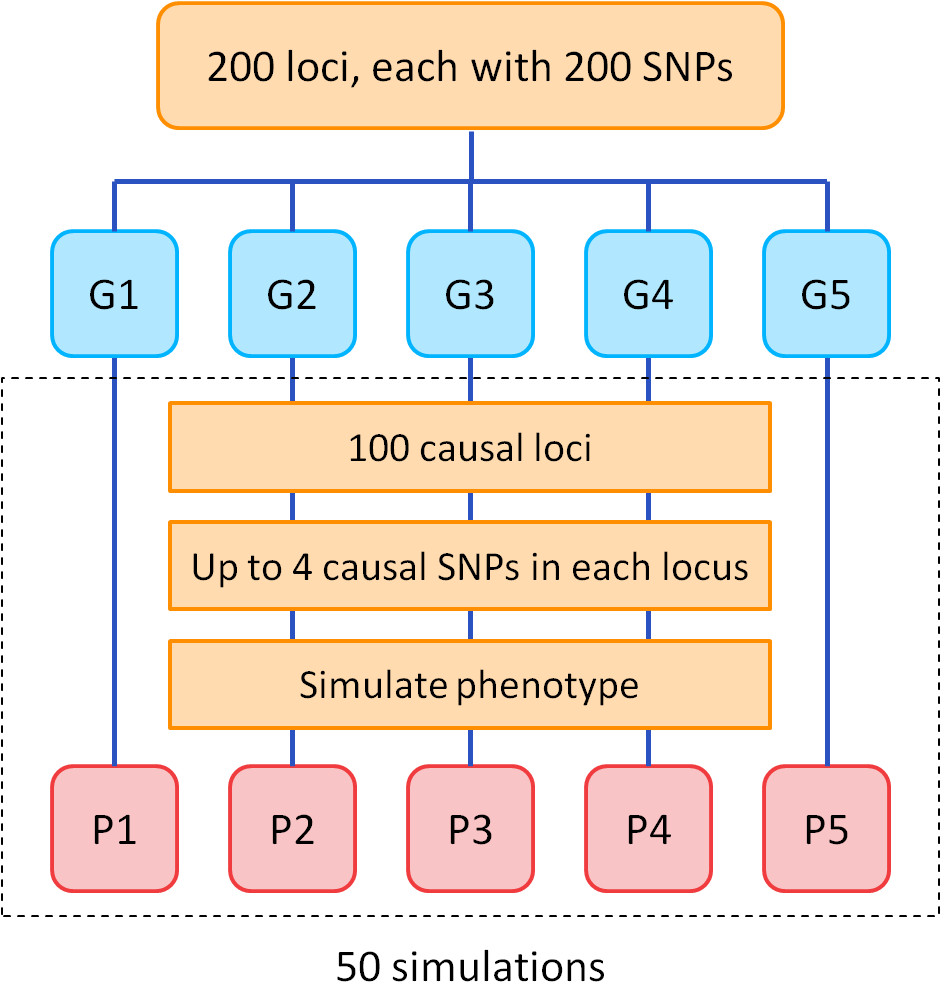
\includegraphics[width=0.86\textwidth]{figures/simulation_details.png}\\
  }{
    \begin{itemize1}
      \item BVSLR
      \item BIMBAM
      \item SNPTEST / META
      \item PAINTOR
    \end{itemize1}
    \vspace{2em}
  }
\end{frame}

\begin{frame}
  \frametitle{Prediction of causal loci}
  \myfulltwocolumn{0.6}{T}
  {
    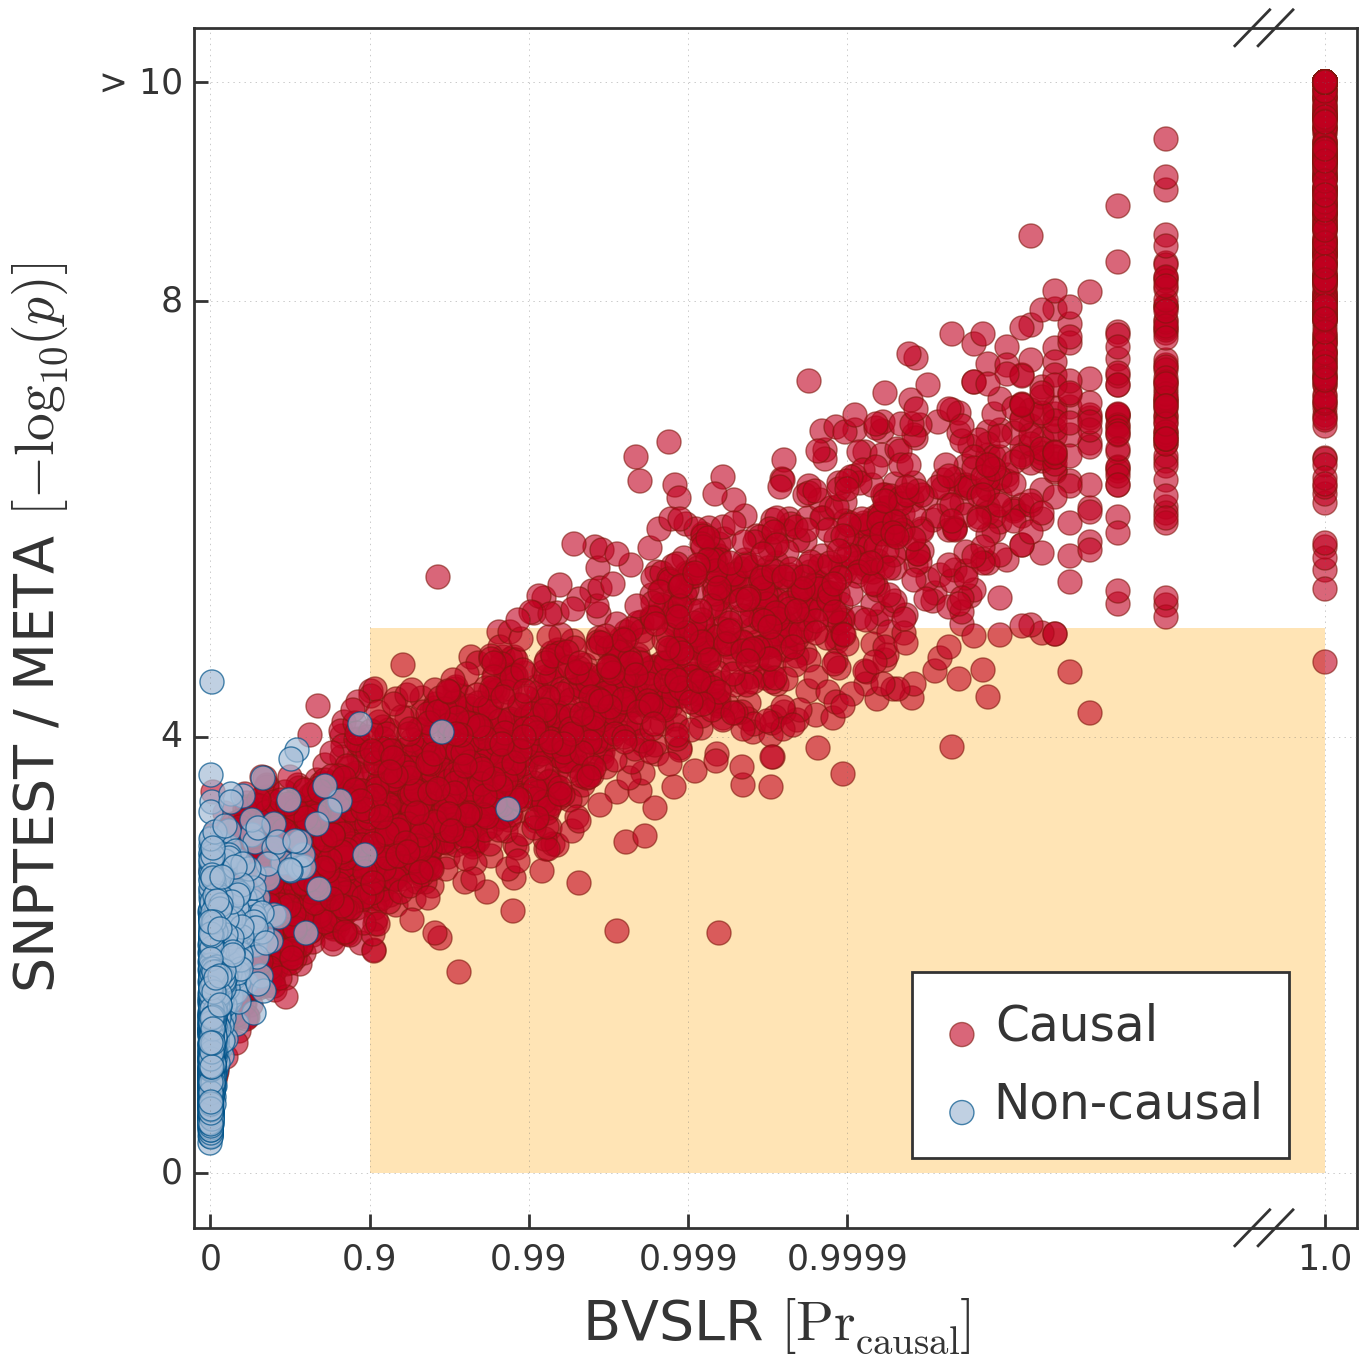
\includegraphics[width=1.0\textwidth]{figures/simu_locus_scatter_nold.png}\\
  }{
    \scriptsize
    \begin{itemize1}
      \item Shaded region shows improvement with BVSLR
      \item 5000 causal loci (100 from each of the 50 simulations)
      \item 5000 non-causal loci (100 from each of the 50 simulations)
    \end{itemize1}
  }
\end{frame}

\begin{frame}
  \frametitle{Prediction of causal loci}
  \myfulltwocolumn{0.6}{T}
  {
    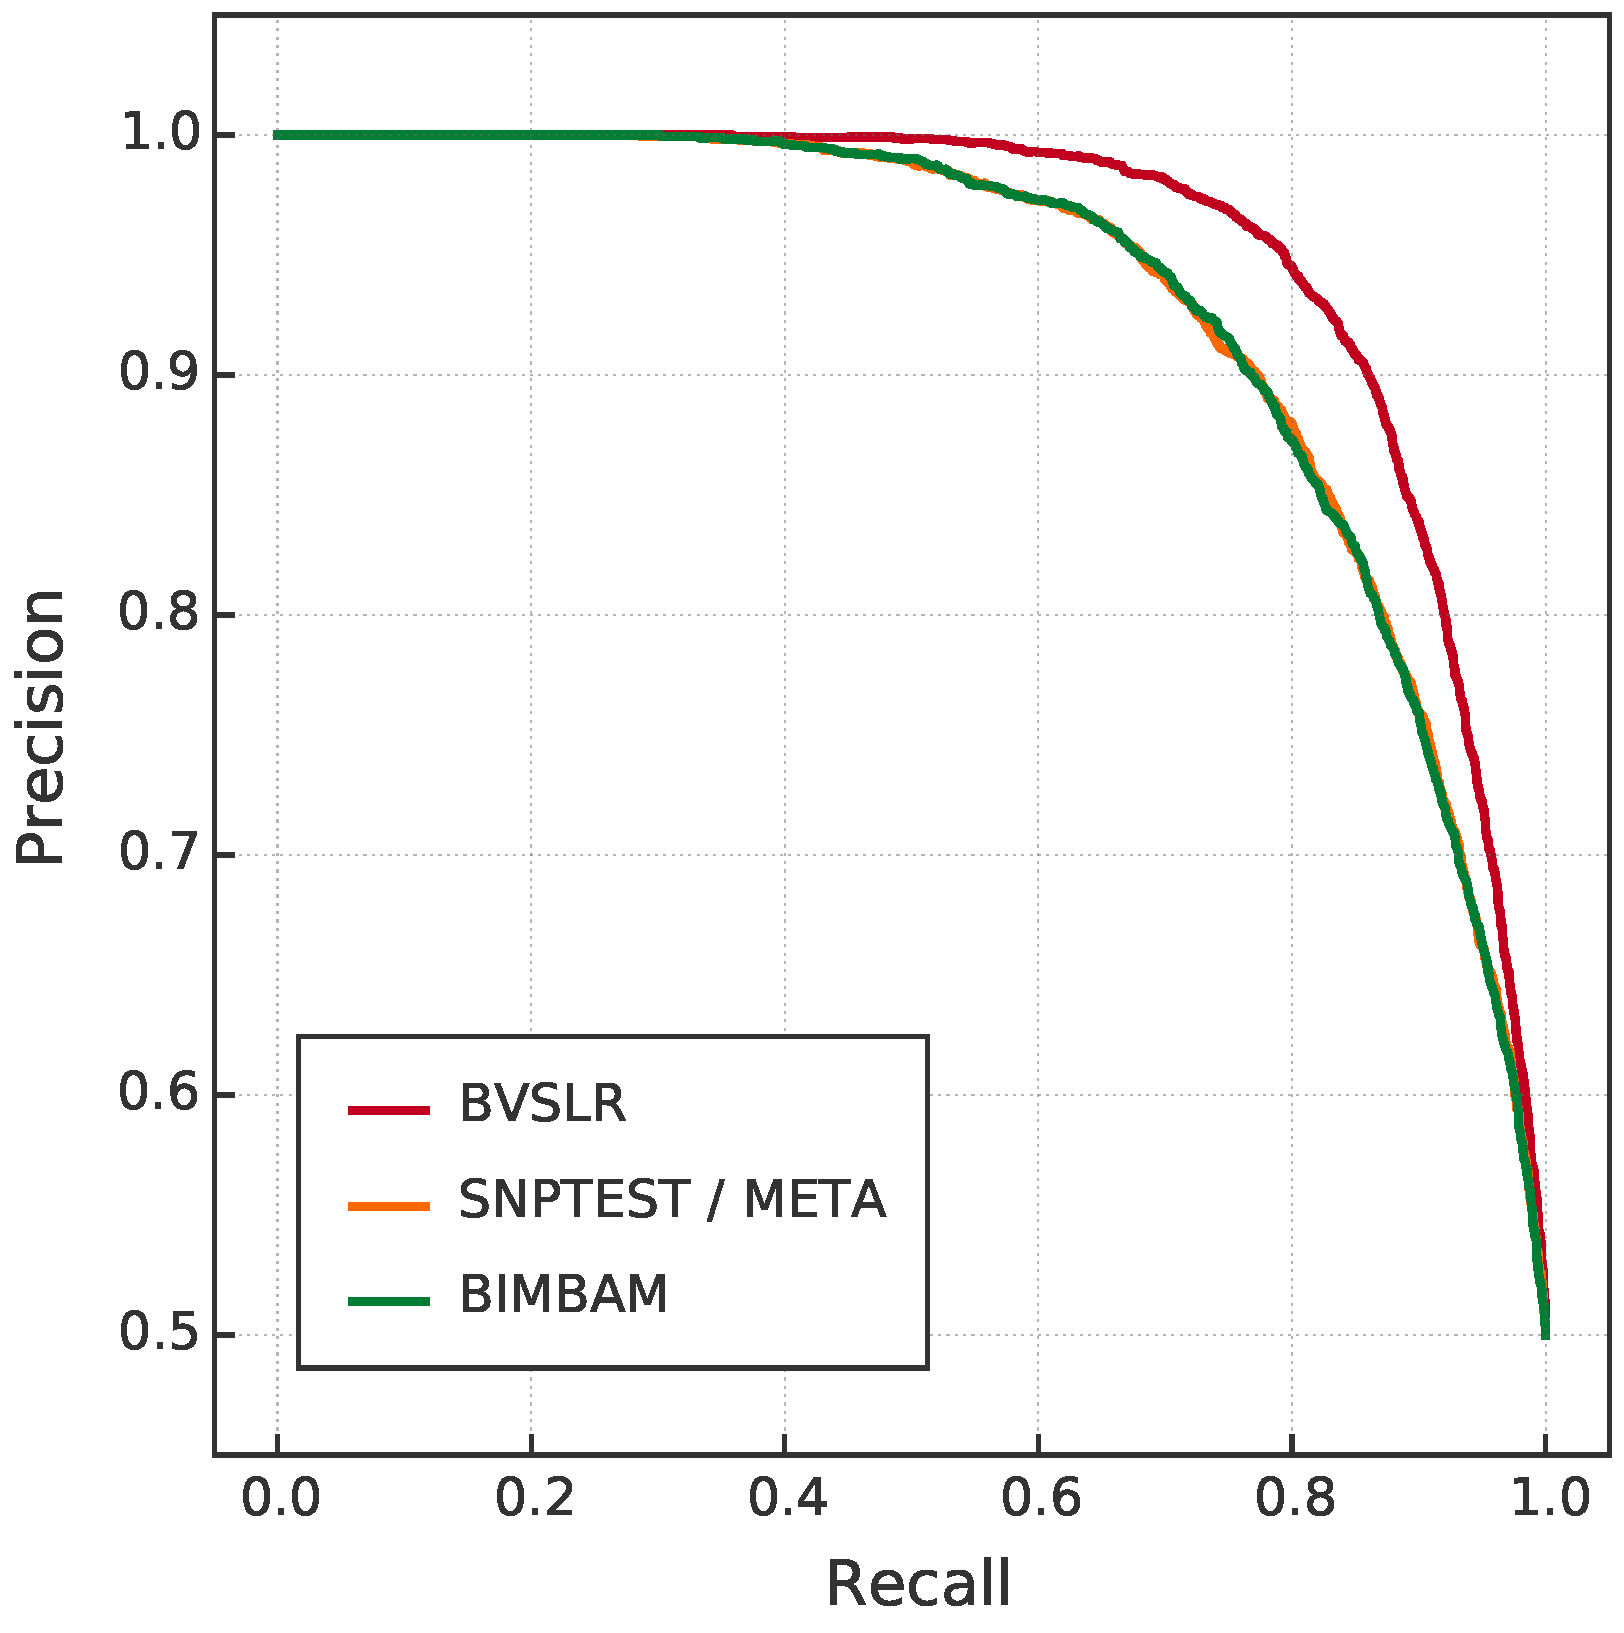
\includegraphics[width=1.0\textwidth]{figures/simu_locus_precision_recall_nold.pdf}\\
  }{
    \begin{align*}
      \text{\scriptsize Precision} & = \frac{\mathrm{TP}}{\mathrm{TP} + \mathrm{FP}} \\
      \text{\scriptsize Recall}    & = \frac{\mathrm{TP}}{\mathrm{TP} + \mathrm{FN}} \\
    \end{align*}
  }
\end{frame}

\begin{frame}
  \frametitle{If there are non-causal loci in LD with causal regions}
  \myfulltwocolumn{0.6}{T}
  {
    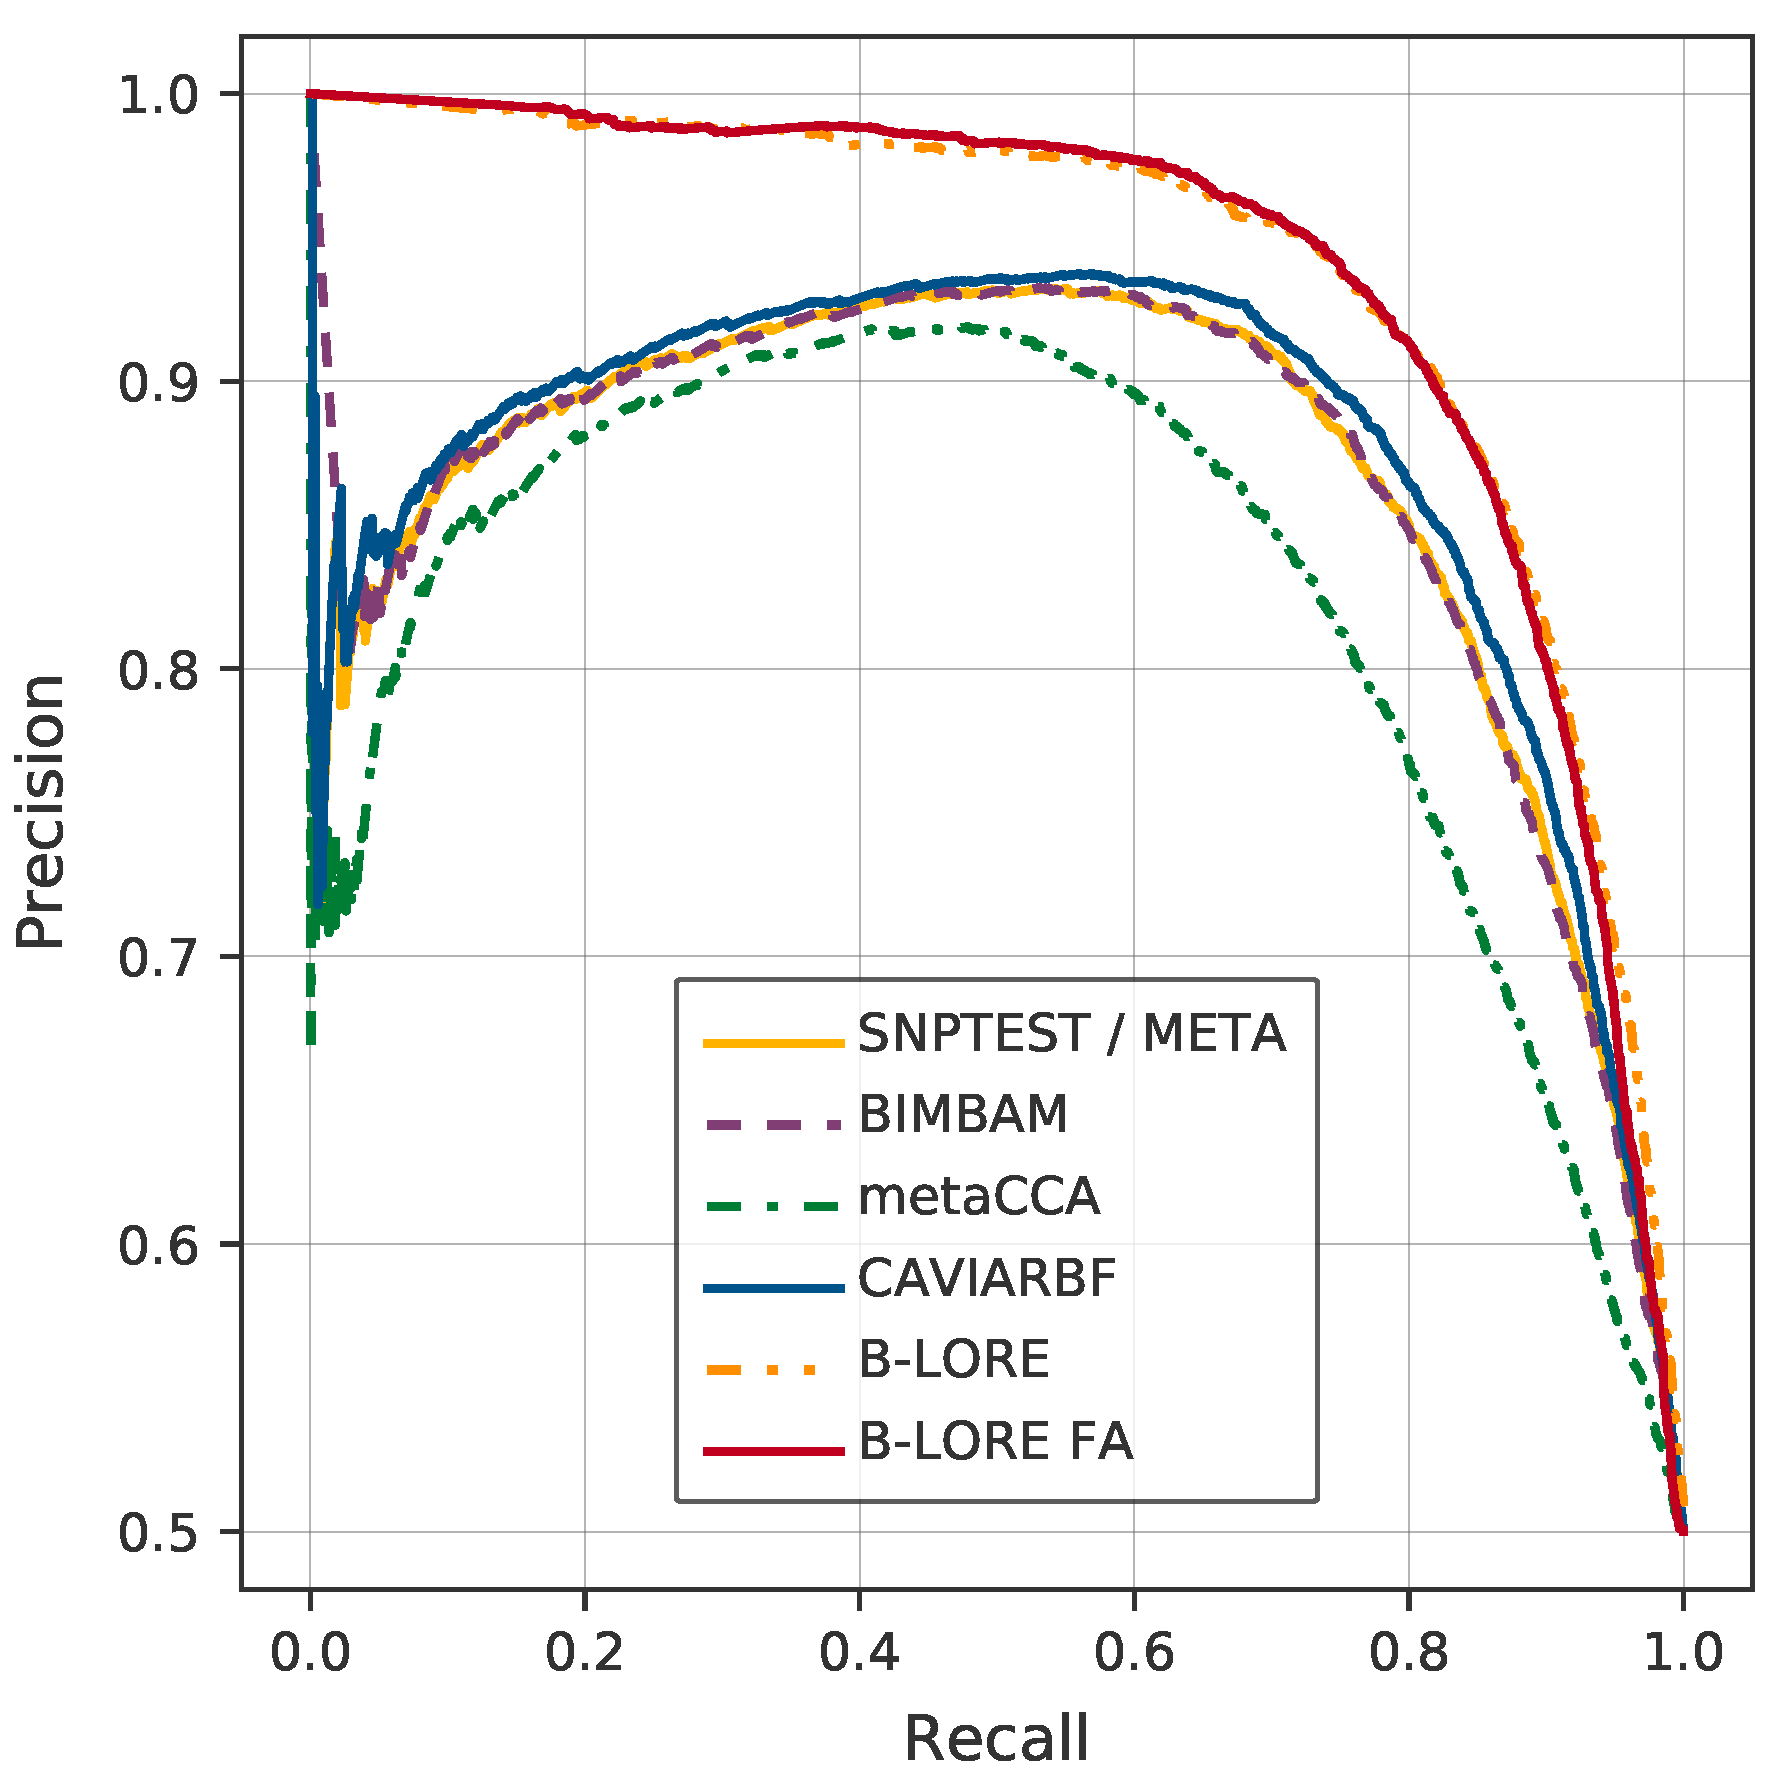
\includegraphics[width=1.0\textwidth]{figures/simu_locus_precision_recall_withld.pdf}\\
  }{
    \begin{align*}
      \text{\scriptsize Precision} & = \frac{\mathrm{TP}}{\mathrm{TP} + \mathrm{FP}} \\
      \text{\scriptsize Recall}    & = \frac{\mathrm{TP}}{\mathrm{TP} + \mathrm{FN}} \\
    \end{align*}
    \begin{itemize1}
      \item 8 loci (out of 200) in LD with each other were introduced in the simulation
    \end{itemize1}
  }
\end{frame}

%\begin{frame}
%  \frametitle{Finemapping causal variants}
%  {\center
%  \vskip -2em
%   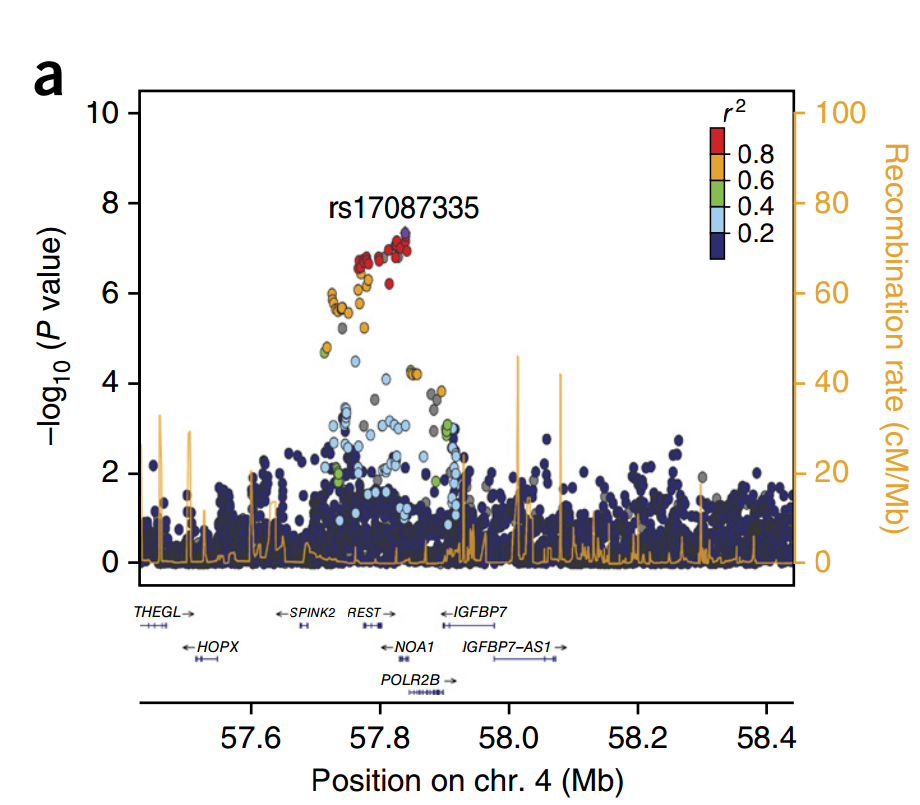
\includegraphics[width=0.6\textwidth]{figures/ng_ss.png} \\
%   Regional association (with CAD) for the 4q12 (REST-NOA1) locus\\
%  }
%  \myreference{Nikpay \etal, \textit{Nat. Gen.} 2015}
%\end{frame}
%
%\begin{frame}
%  \frametitle{Finemapping causal variants}
%  \begin{itemize1}
%    \item Requires significant coverage of genotyped / imputed SNPs at the causal loci
%    \item Putatively causal SNPs can be functionally tested (laborious and expensive)
%    \item Traditional statistical approach: iteratively calculates p-values by conditioning on the most significantly associated SNP(s)
%    \item Recent methods, like PAINTOR and CAVIARBF uses LD information to resolve causal variants
%    \item PAINTOR can additionally use functional annotations
%  \end{itemize1}
%\end{frame}

\begin{frame}
  \frametitle{Finemapping causal variants}
  \myfulltwocolumn{0.6}{T}
  {
    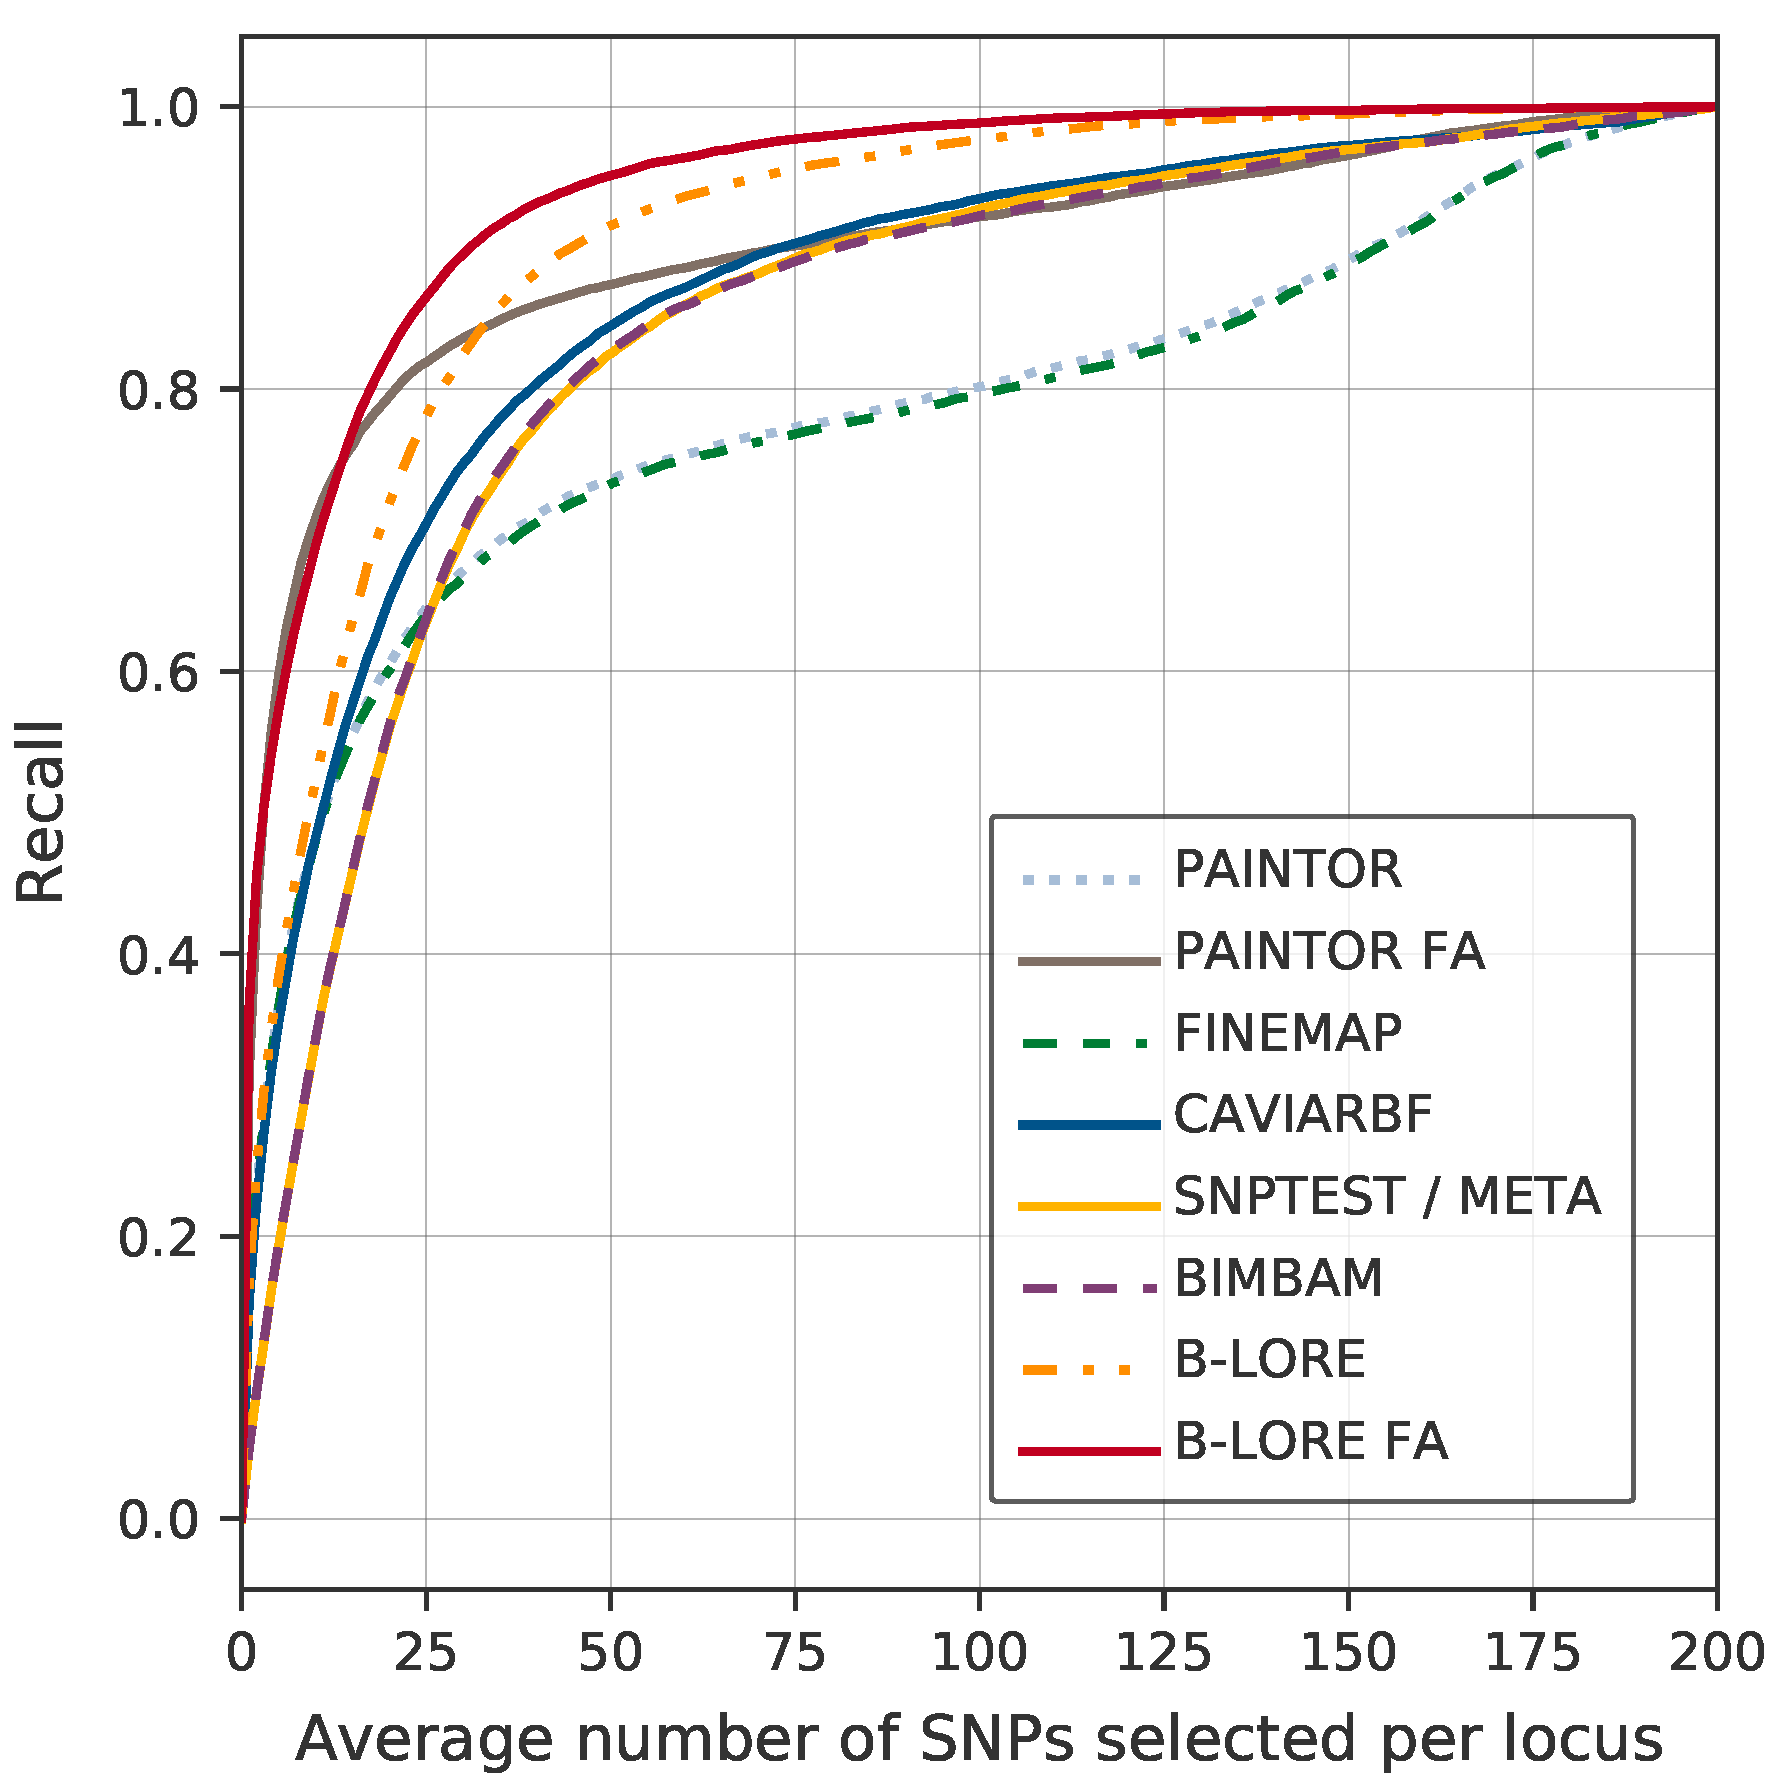
\includegraphics[width=1.0\textwidth]{figures/simu_finemap_recall_nold.pdf}\\
  }{
    \begin{itemize1}
      \item Comparable to PAINTOR up to 20\% recall
    \end{itemize1}
  }
\end{frame}

\begin{frame}
  \frametitle{BVSLR predicts SNPs in strong LD with actual ones}
  \mytwocolumn{0.5}{T}
  {
    \center
    \vskip -2em
    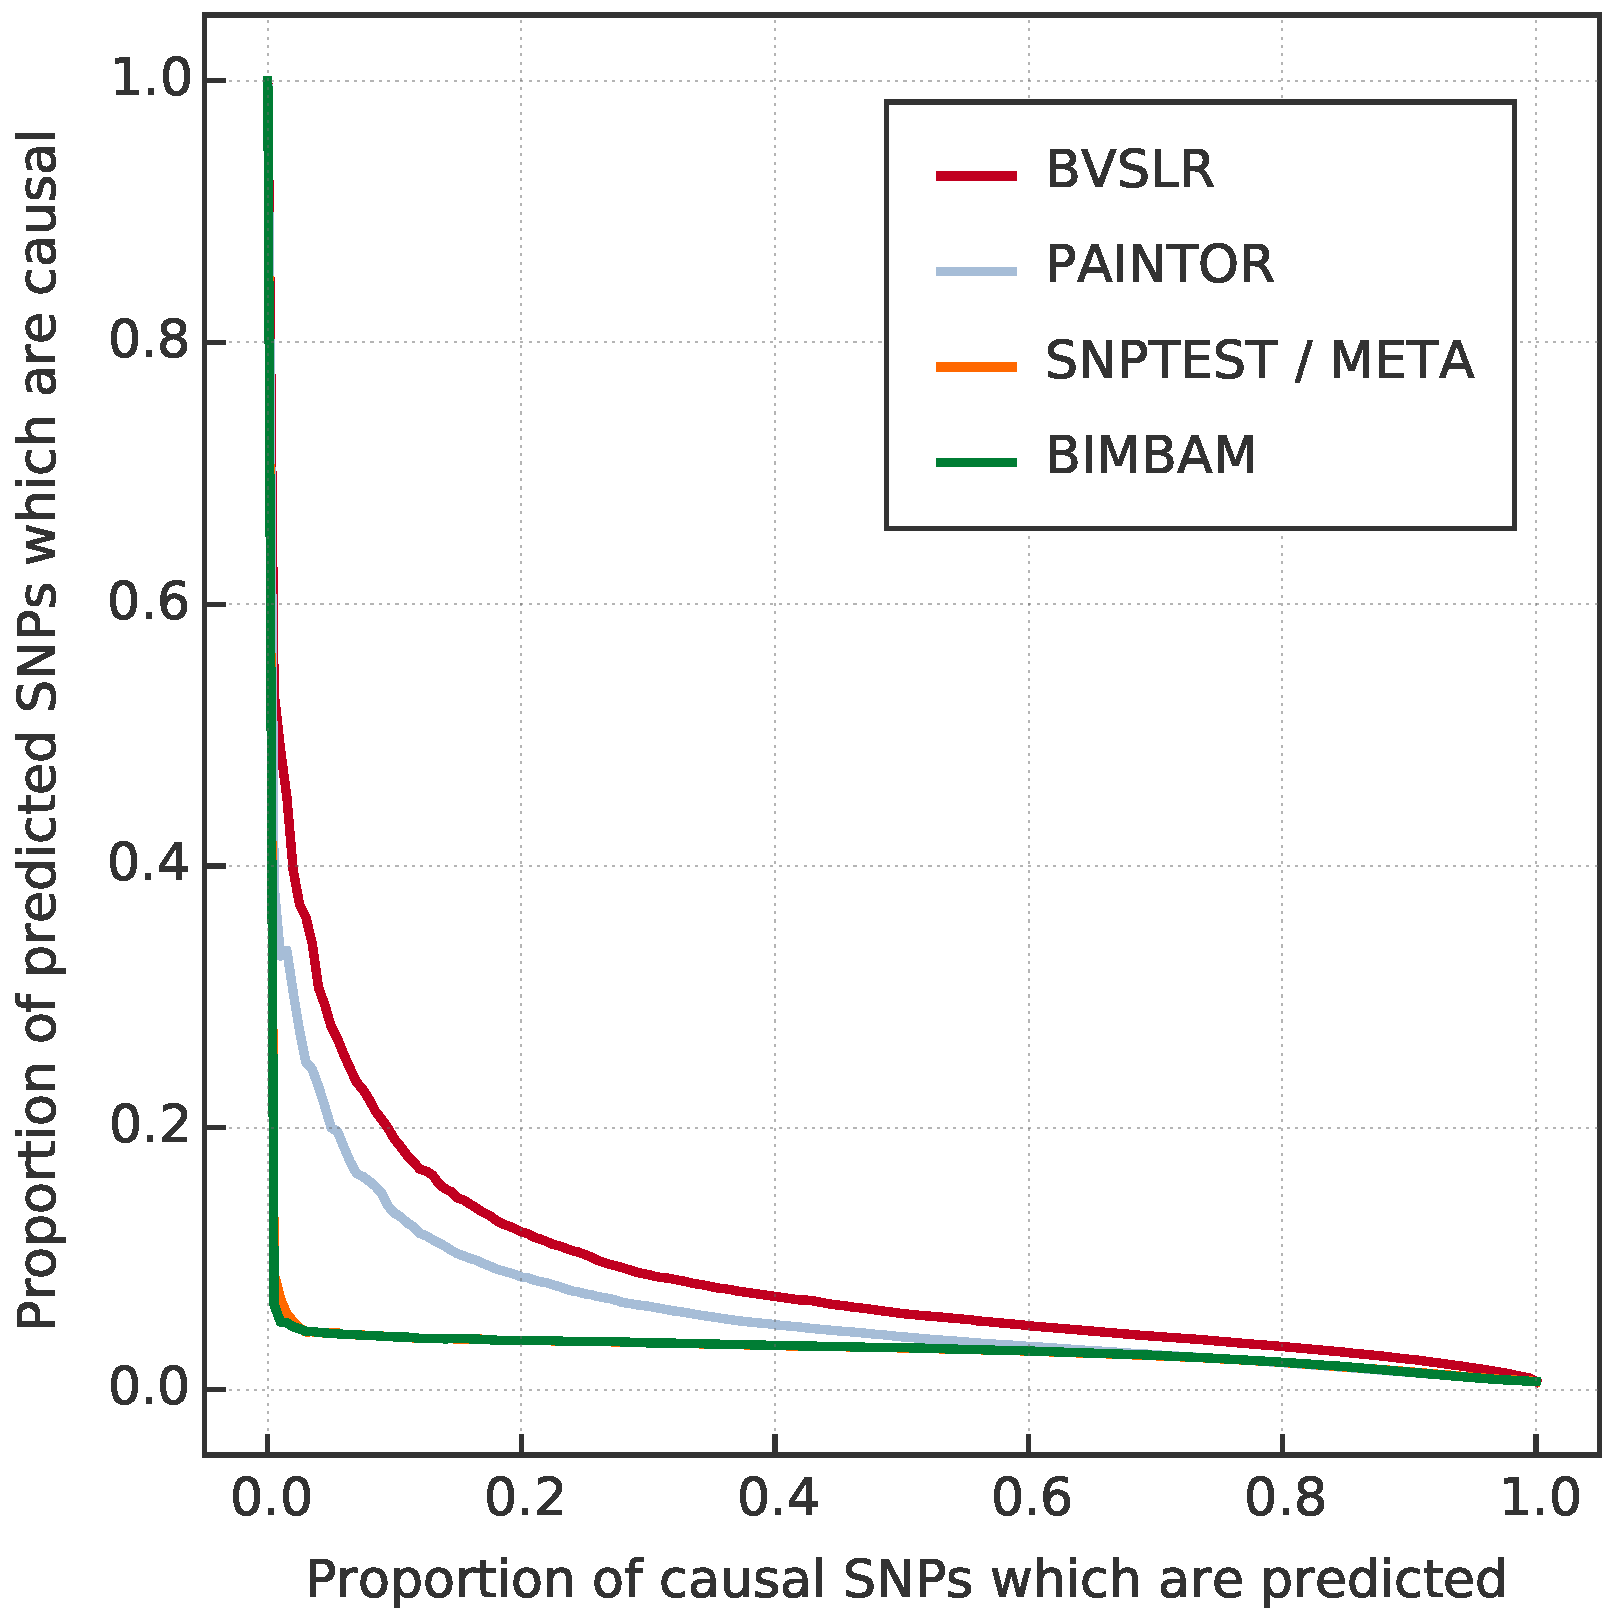
\includegraphics[width=1.0\textwidth]{figures/simu_finemap_precision_recall01_nold.pdf} \\
  }{
    \center
    \vskip -2em
    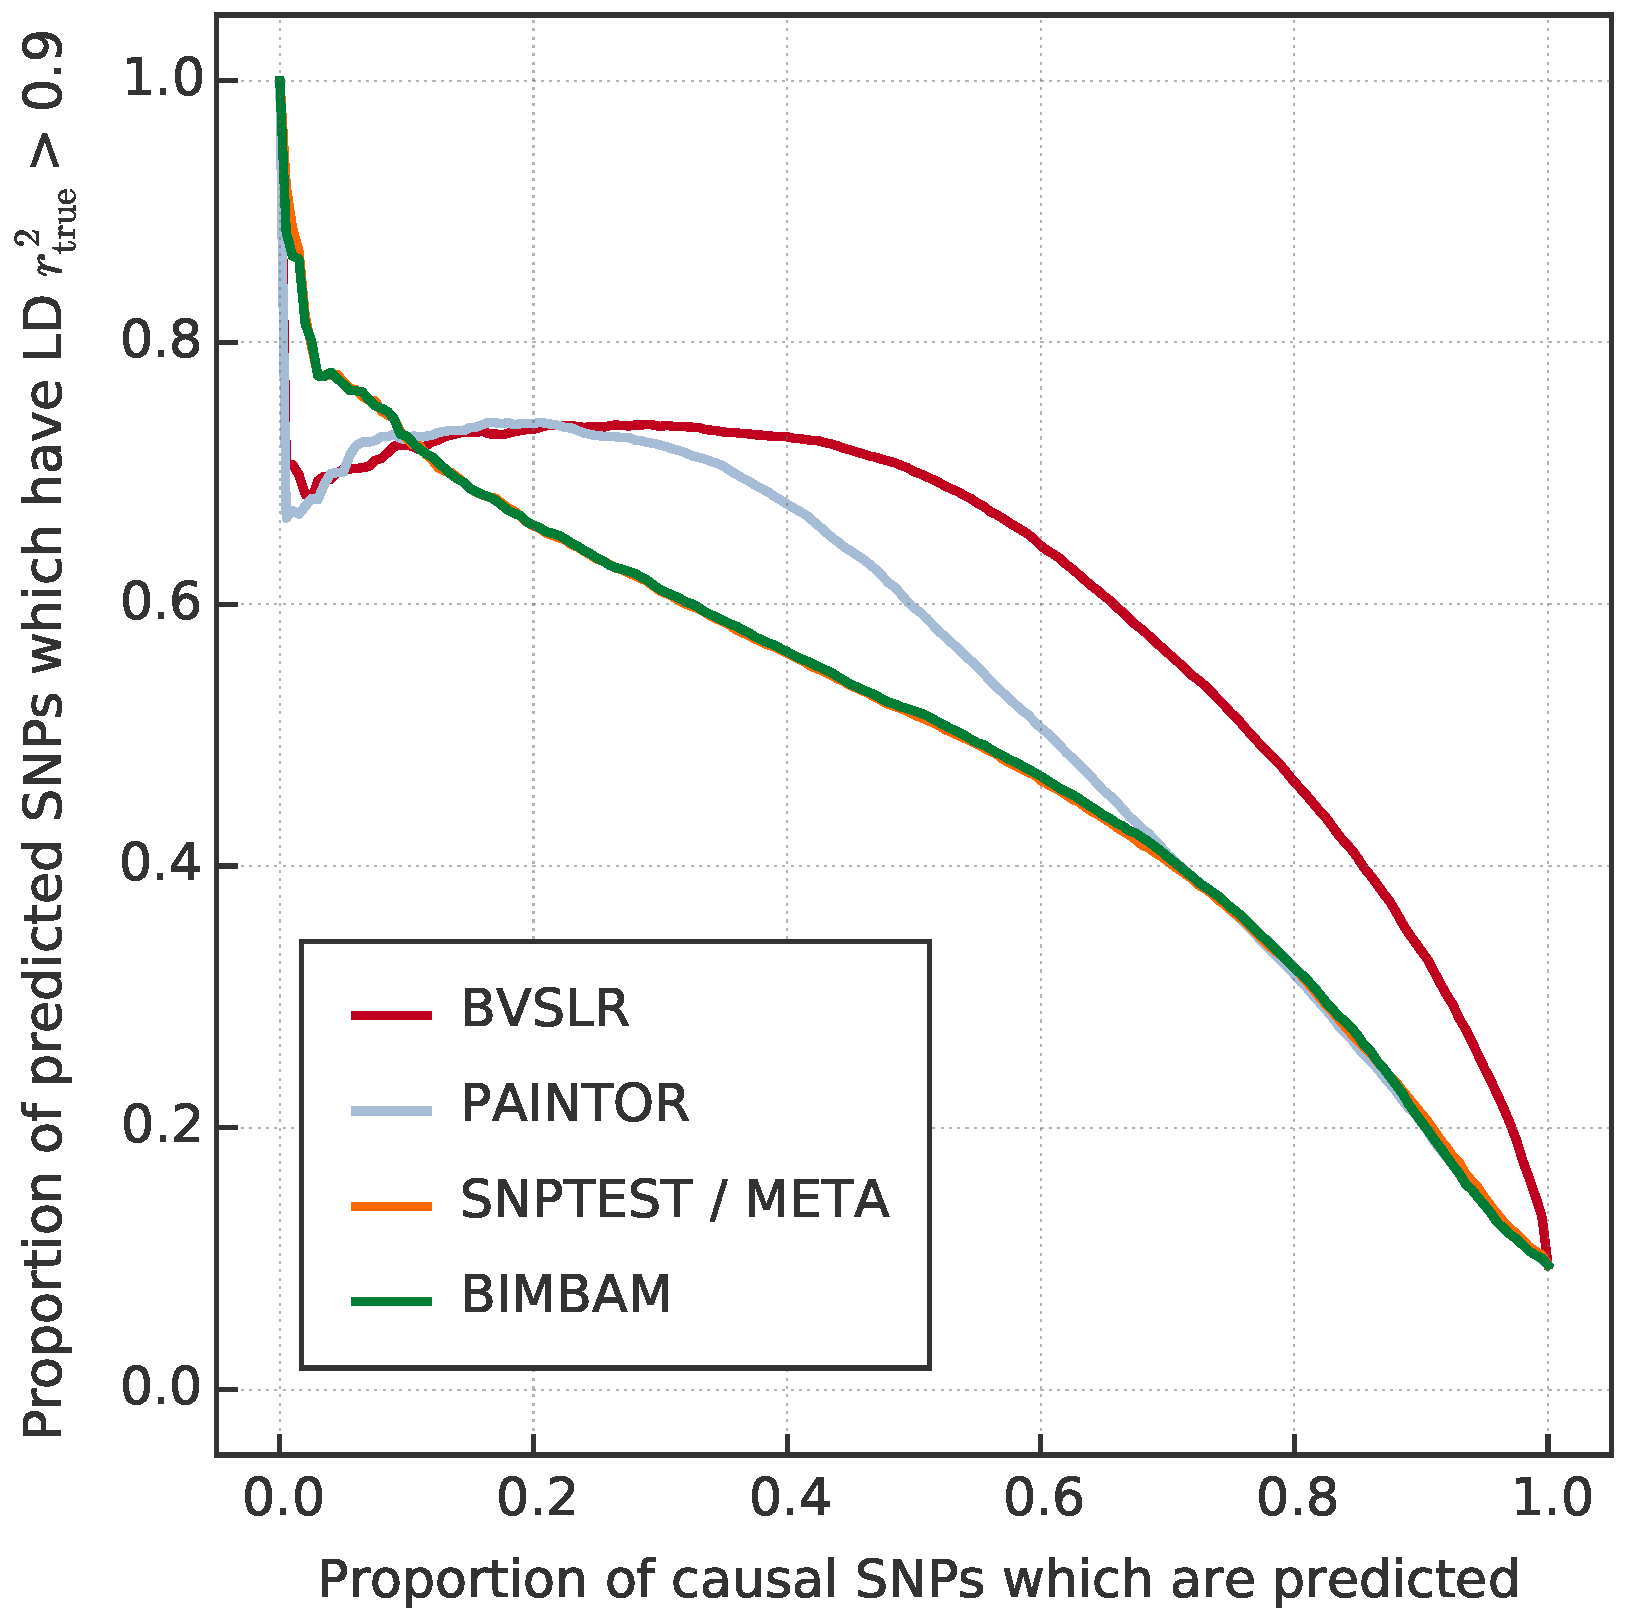
\includegraphics[width=1.0\textwidth]{figures/simu_finemap_precision_recall02_nold.pdf}\\
  }
\end{frame}

% \begin{frame}
%   \frametitle{Challenges of BVSLR}
%   \begin{itemize1}
%     \item Computational time (summing over $\vz$-states)
%     \item New summary statistics
%     \item Prior assumptions
%   \end{itemize1}
% \end{frame}

\subsection{Coronary Artery Diseases}

\begin{frame}
  \frametitle{Association with coronary artery diseases (CAD)}
  \begin{itemize1}
    \item 5 GERMIFS cohorts
    \item 6228 cases, 6854 controls
    \item Imputed with 1000G Phase 1
  \end{itemize1}
  \uncover<2->
  {\center
   %\vskip -2em
   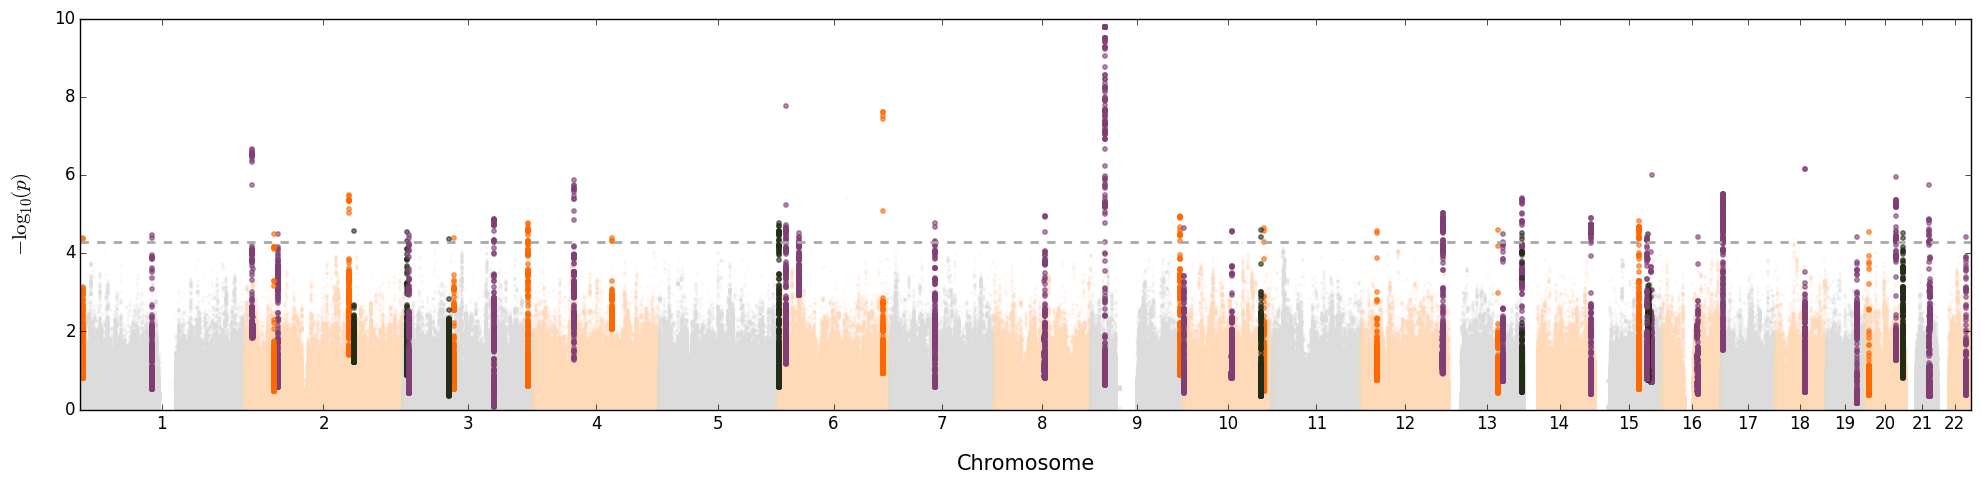
\includegraphics[width=1.0\textwidth]{figures/cad_gwas_germifs.png} \\
   GWAS using SNPTEST / META \\
  }
  \vskip 1em
  \uncover<3->{
  \begin{itemize1}
    \item Applied BVSLR on these 45 loci, selecting 400 SNPs at each locus.
  \end{itemize1}
  }
\end{frame}

\begin{frame}
  \frametitle{BVSLR predictions}
  {\center
  \vskip -1em
   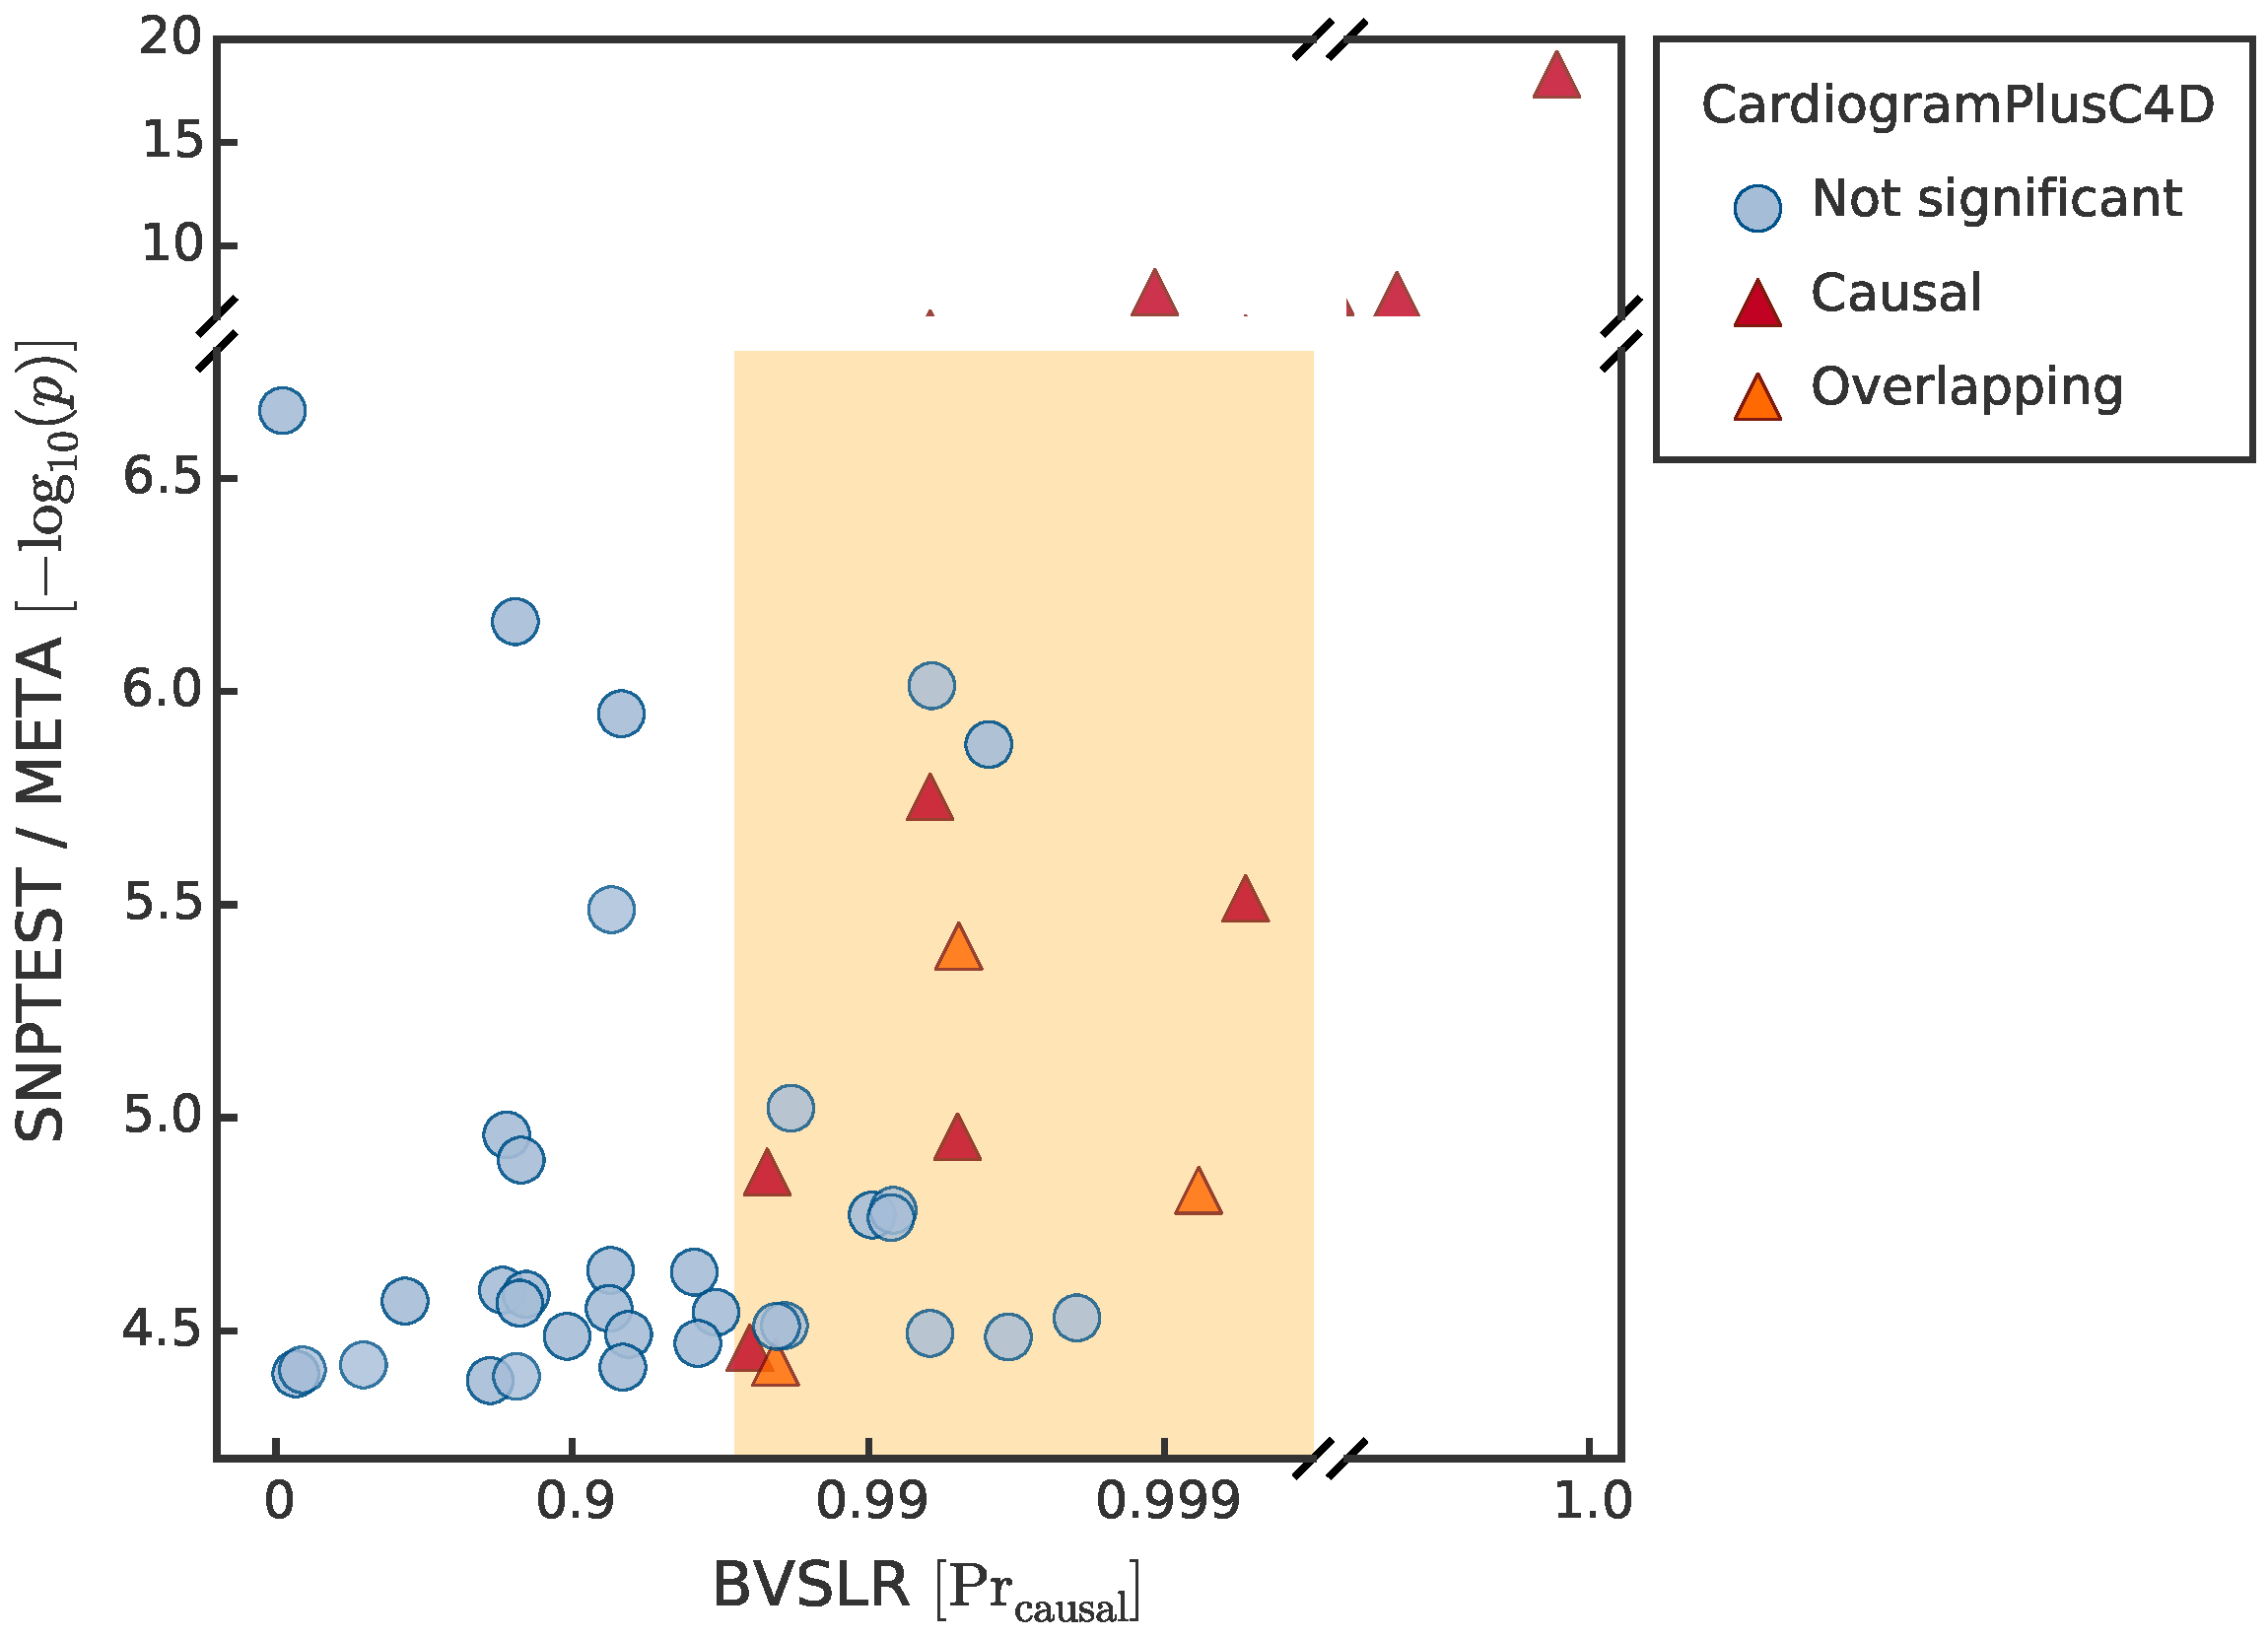
\includegraphics[width=0.9\textwidth]{figures/loci_classification_01.pdf} \\
  }
\end{frame}

\begin{frame}
  \frametitle{Top BVSLR predicted loci (not discovered in CardiogramPlusC4D)}
  \vskip -2em
  {\center \scriptsize
    \def\arraystretch{1.5}
    \begin{tabular}{ c c c c l }
      \rowcolor{highlight!20}
      Region  & $Pr$   & Gene & Comments \\
      \rowcolor{secondary!30}
      6p21.3  & 0.998  & C6orf10-BTNL2 & GWAS for CAD in Han Chinese, 2012 \\
      \rowcolor{secondary!30}
      15q25   & 0.997  & IL-16 & GWAS for CAD in Han Chinese, 2012 \\
      4q13.1  & 0.996  & desert & -- \\
      \rowcolor{secondary!15}
      15q25   & 0.994  & AKAP13 & C. hypertrophy (mice) / GWAS (BP in Koreans, 2011) \\
      \rowcolor{secondary!30}
      2p16    & 0.994  & NRXN1   & GWAS for CAD in OHGS1 + WTCCC2 \\
      \rowcolor{secondary!15}
      3q28    & 0.992  & IL1RAP & Involved in risk pathway \\
      \rowcolor{secondary!15}
      6p25    & 0.992  & SERPINB & patented as biomarker for CVD \\
      \rowcolor{secondary!30}
      20q13.3 & 0.991  & EDN3    & GWAS hit for BP / CVD \\
      7q11.22 & 0.990  & AUTS2  & -- \\
      \rowcolor{secondary!15}
      12q24   & 0.982  & ZNF664 & GWAS hit for HDL-C, TG \\
      \rowcolor{secondary!15}
      13q21.1 & 0.981  & ARHGEF1 & Controls vascular tone and BP \\
    \end{tabular}
  \\}
\end{frame}

\begin{frame}
  \frametitle{Literature-based classification}
  {\center
  \vskip -1em
   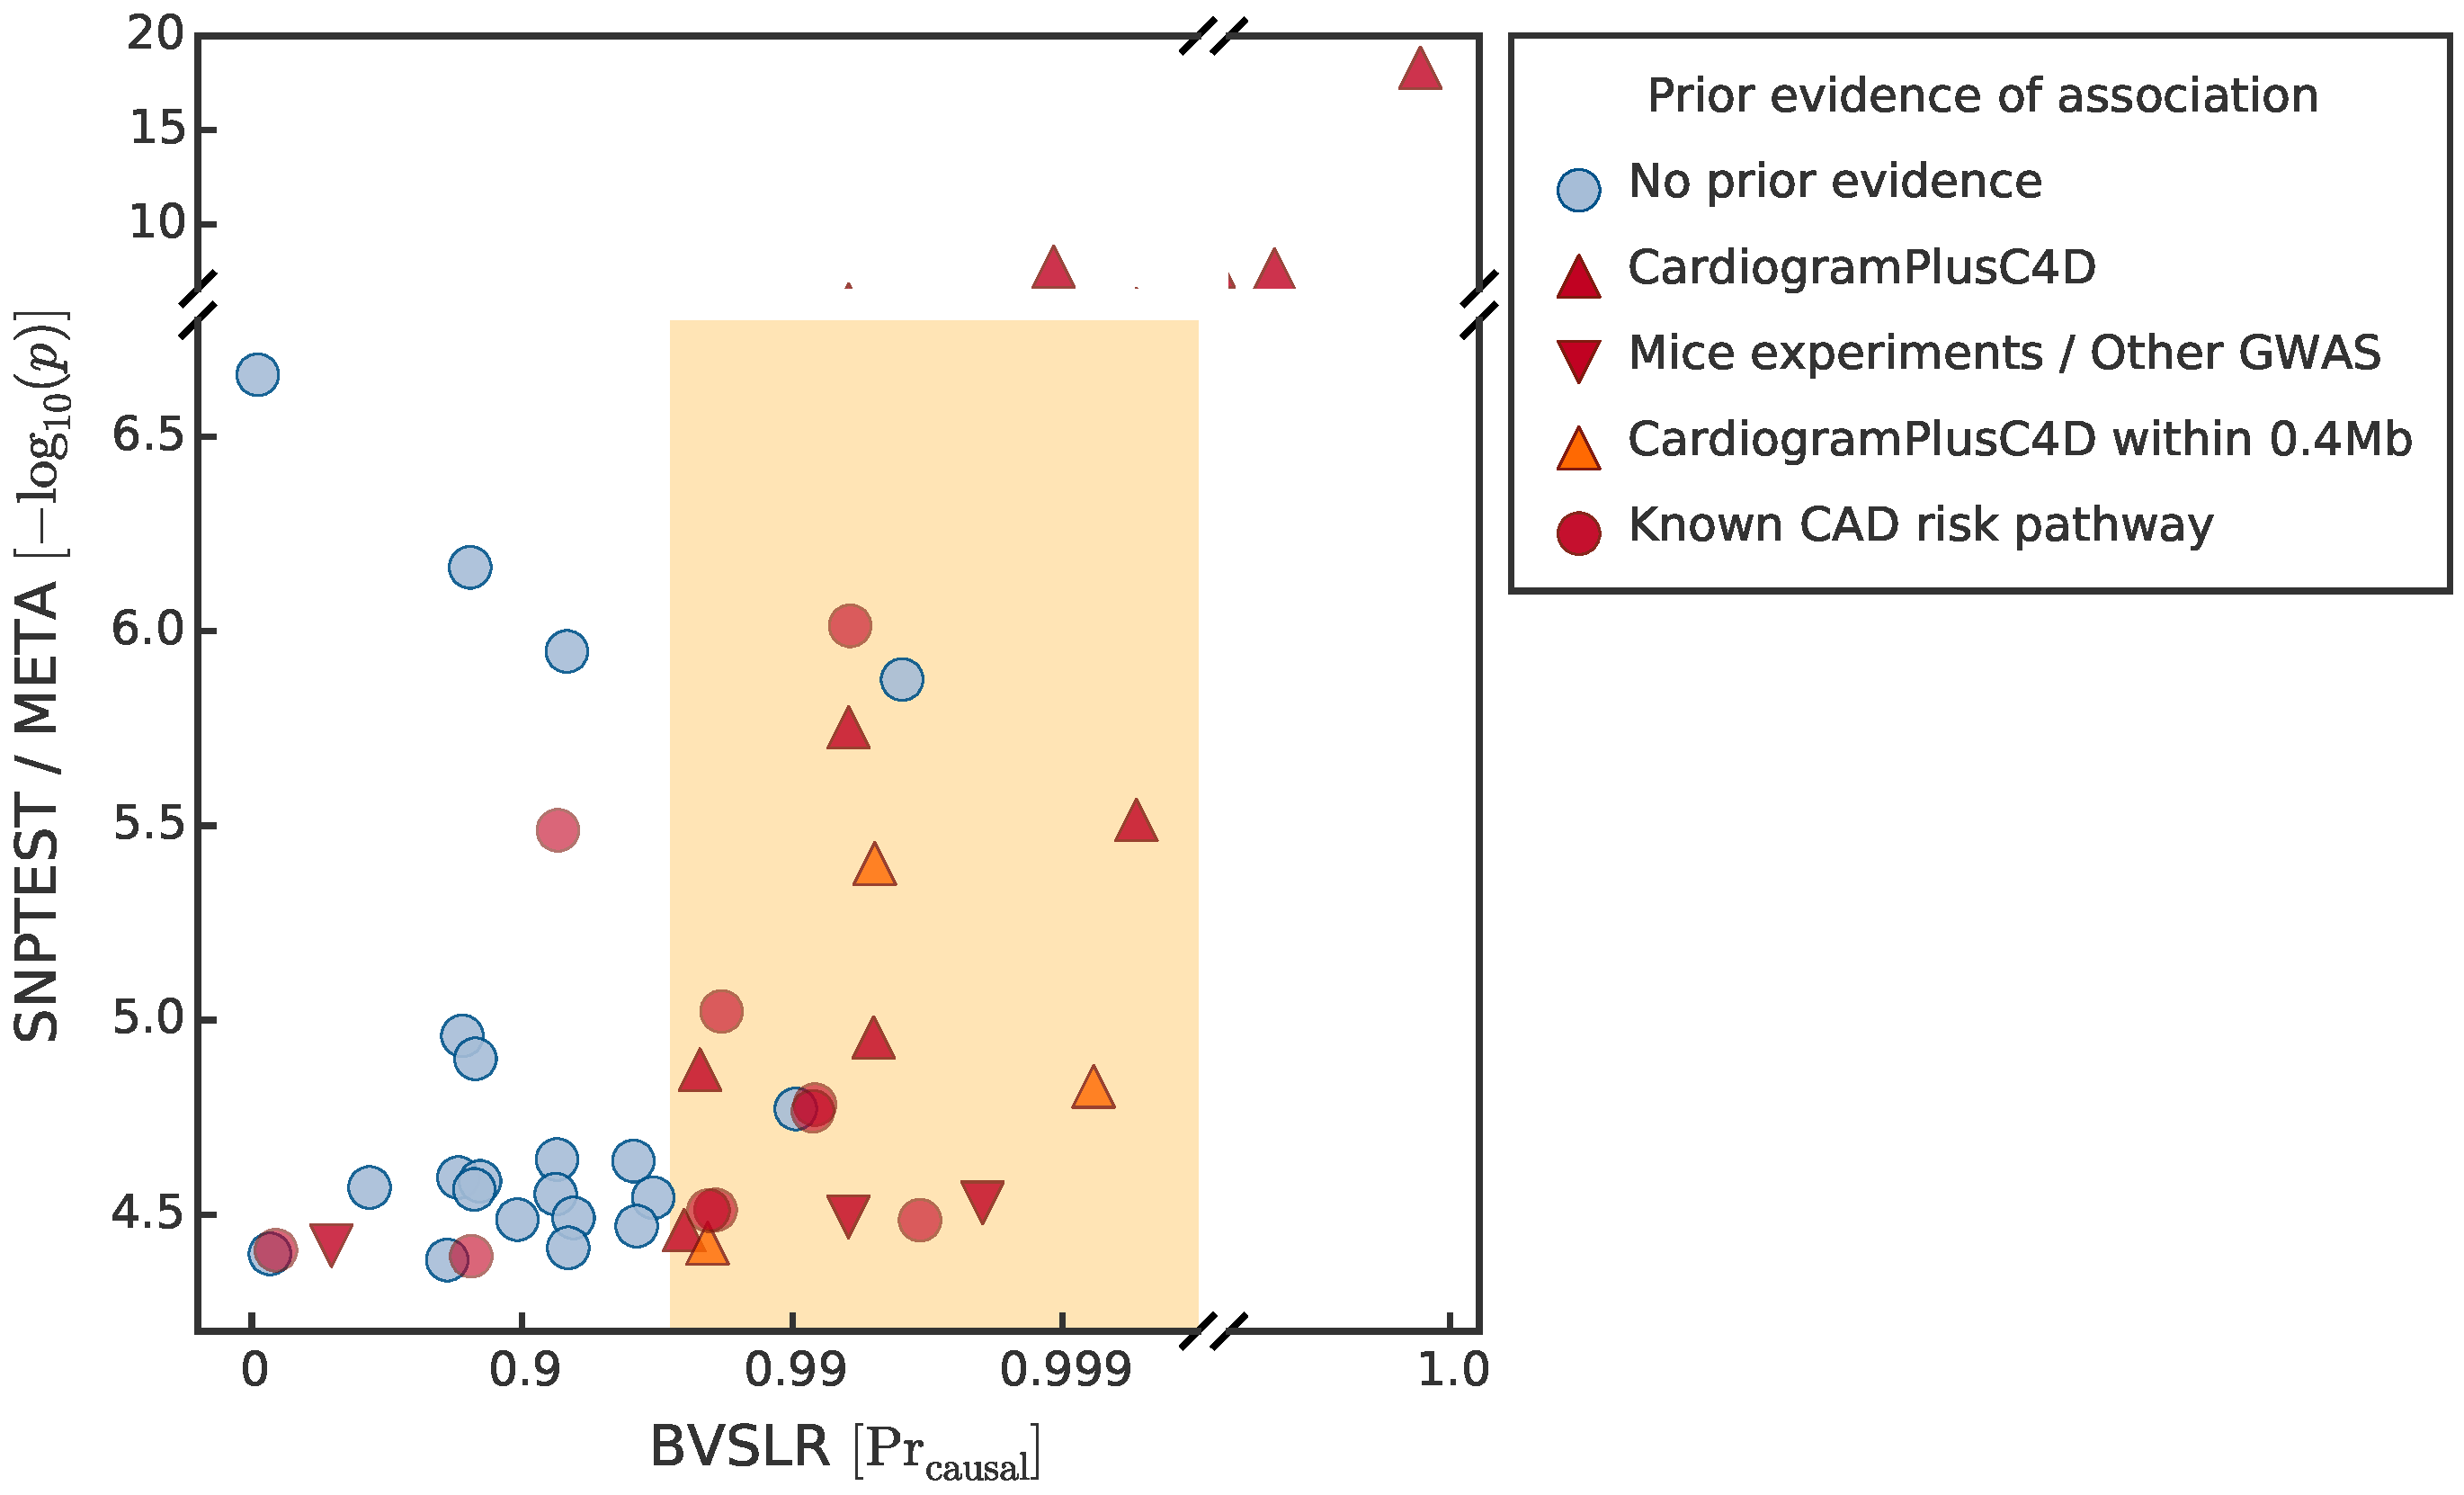
\includegraphics[width=0.9\textwidth]{figures/loci_classification_03.pdf} \\
  }
\end{frame}

% \begin{frame}
%   \frametitle{Essence}
%   \begin{itemize1}
%     \item Novel Bayesian method for GWAS
%     \item Multivariate analysis in meta studies
%     \item Precision
%     \item Predicts new associations in CAD
%     %\item<2-> Actively looking forward to real data to apply BVSLR
%   \end{itemize1}
% \end{frame}
% 
% \begin{frame}
%   \frametitle{Many thanks to \ldots}
%   \tiny
%   \begin{columns}[t]
%     \begin{column}{0.15\textwidth}
%       \center
%       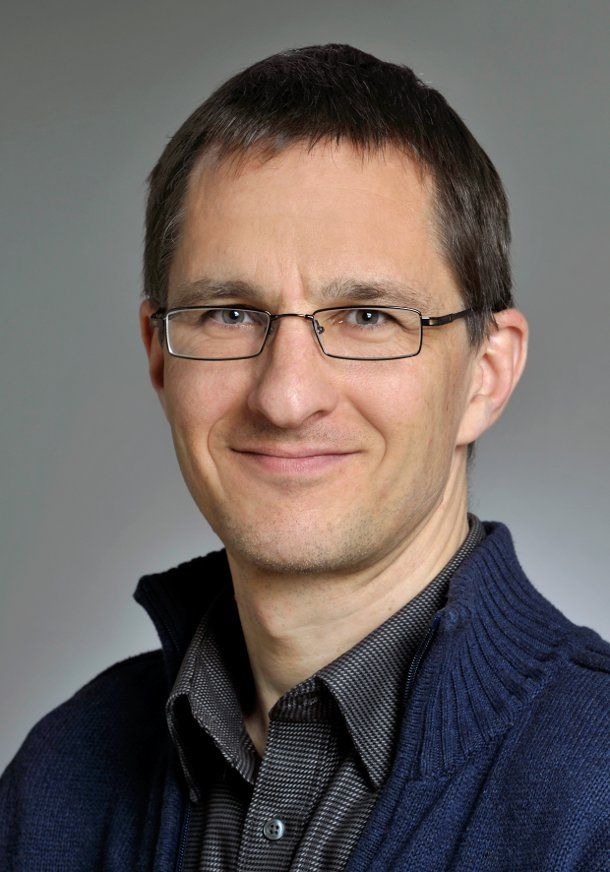
\includegraphics[height=0.25\textheight]{figures/soeding.jpg} \\
%       Johannes S\"oding \\
%     \end{column}
%     \begin{column}{0.15\textwidth}
%       \center
%       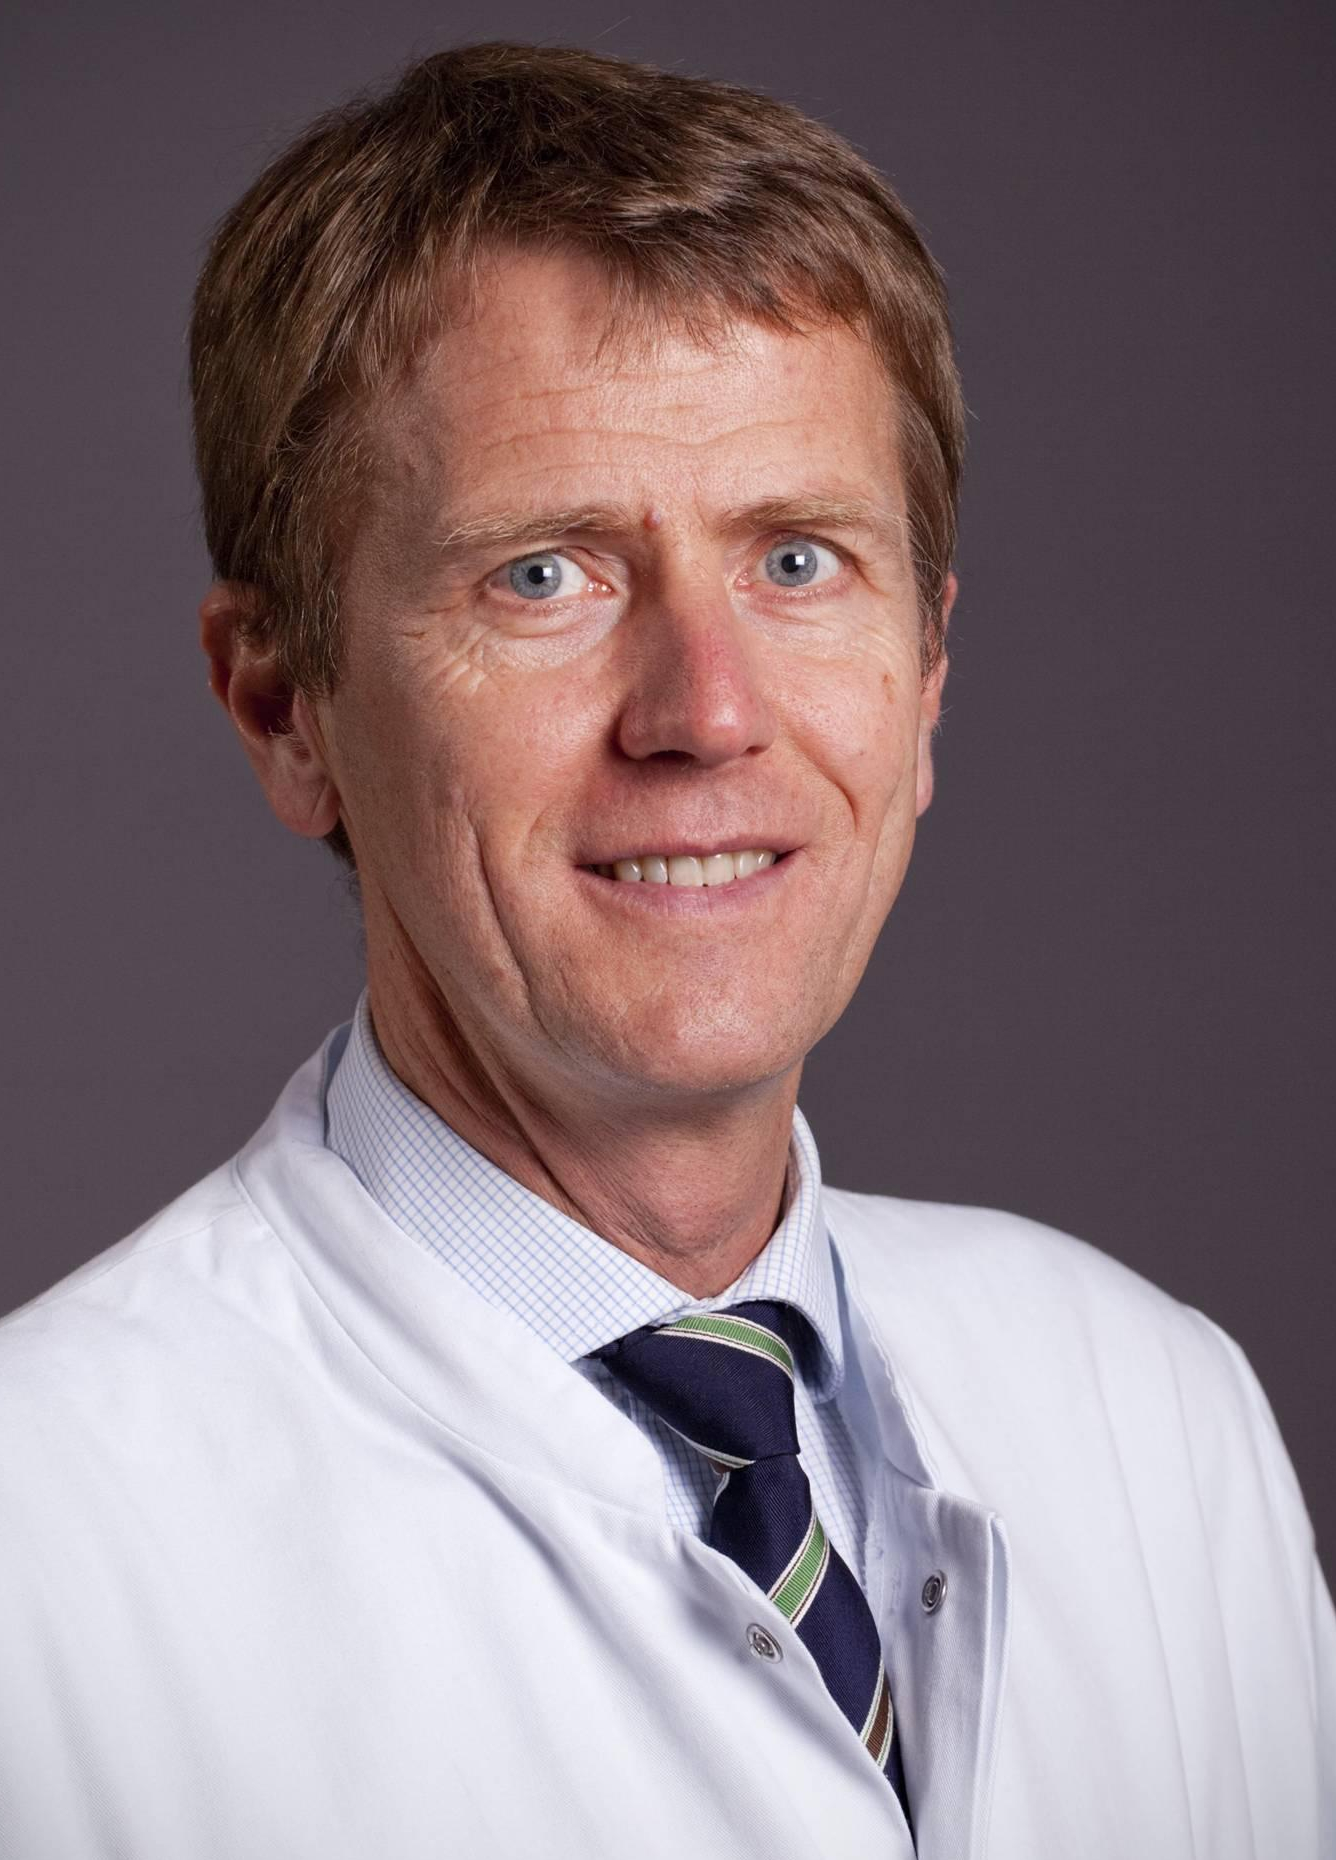
\includegraphics[height=0.25\textheight]{figures/schunkert.jpg} \\
%       Heribert Schunkert \\
%     \end{column}
%     \begin{column}{0.15\textwidth}
%       \center
%       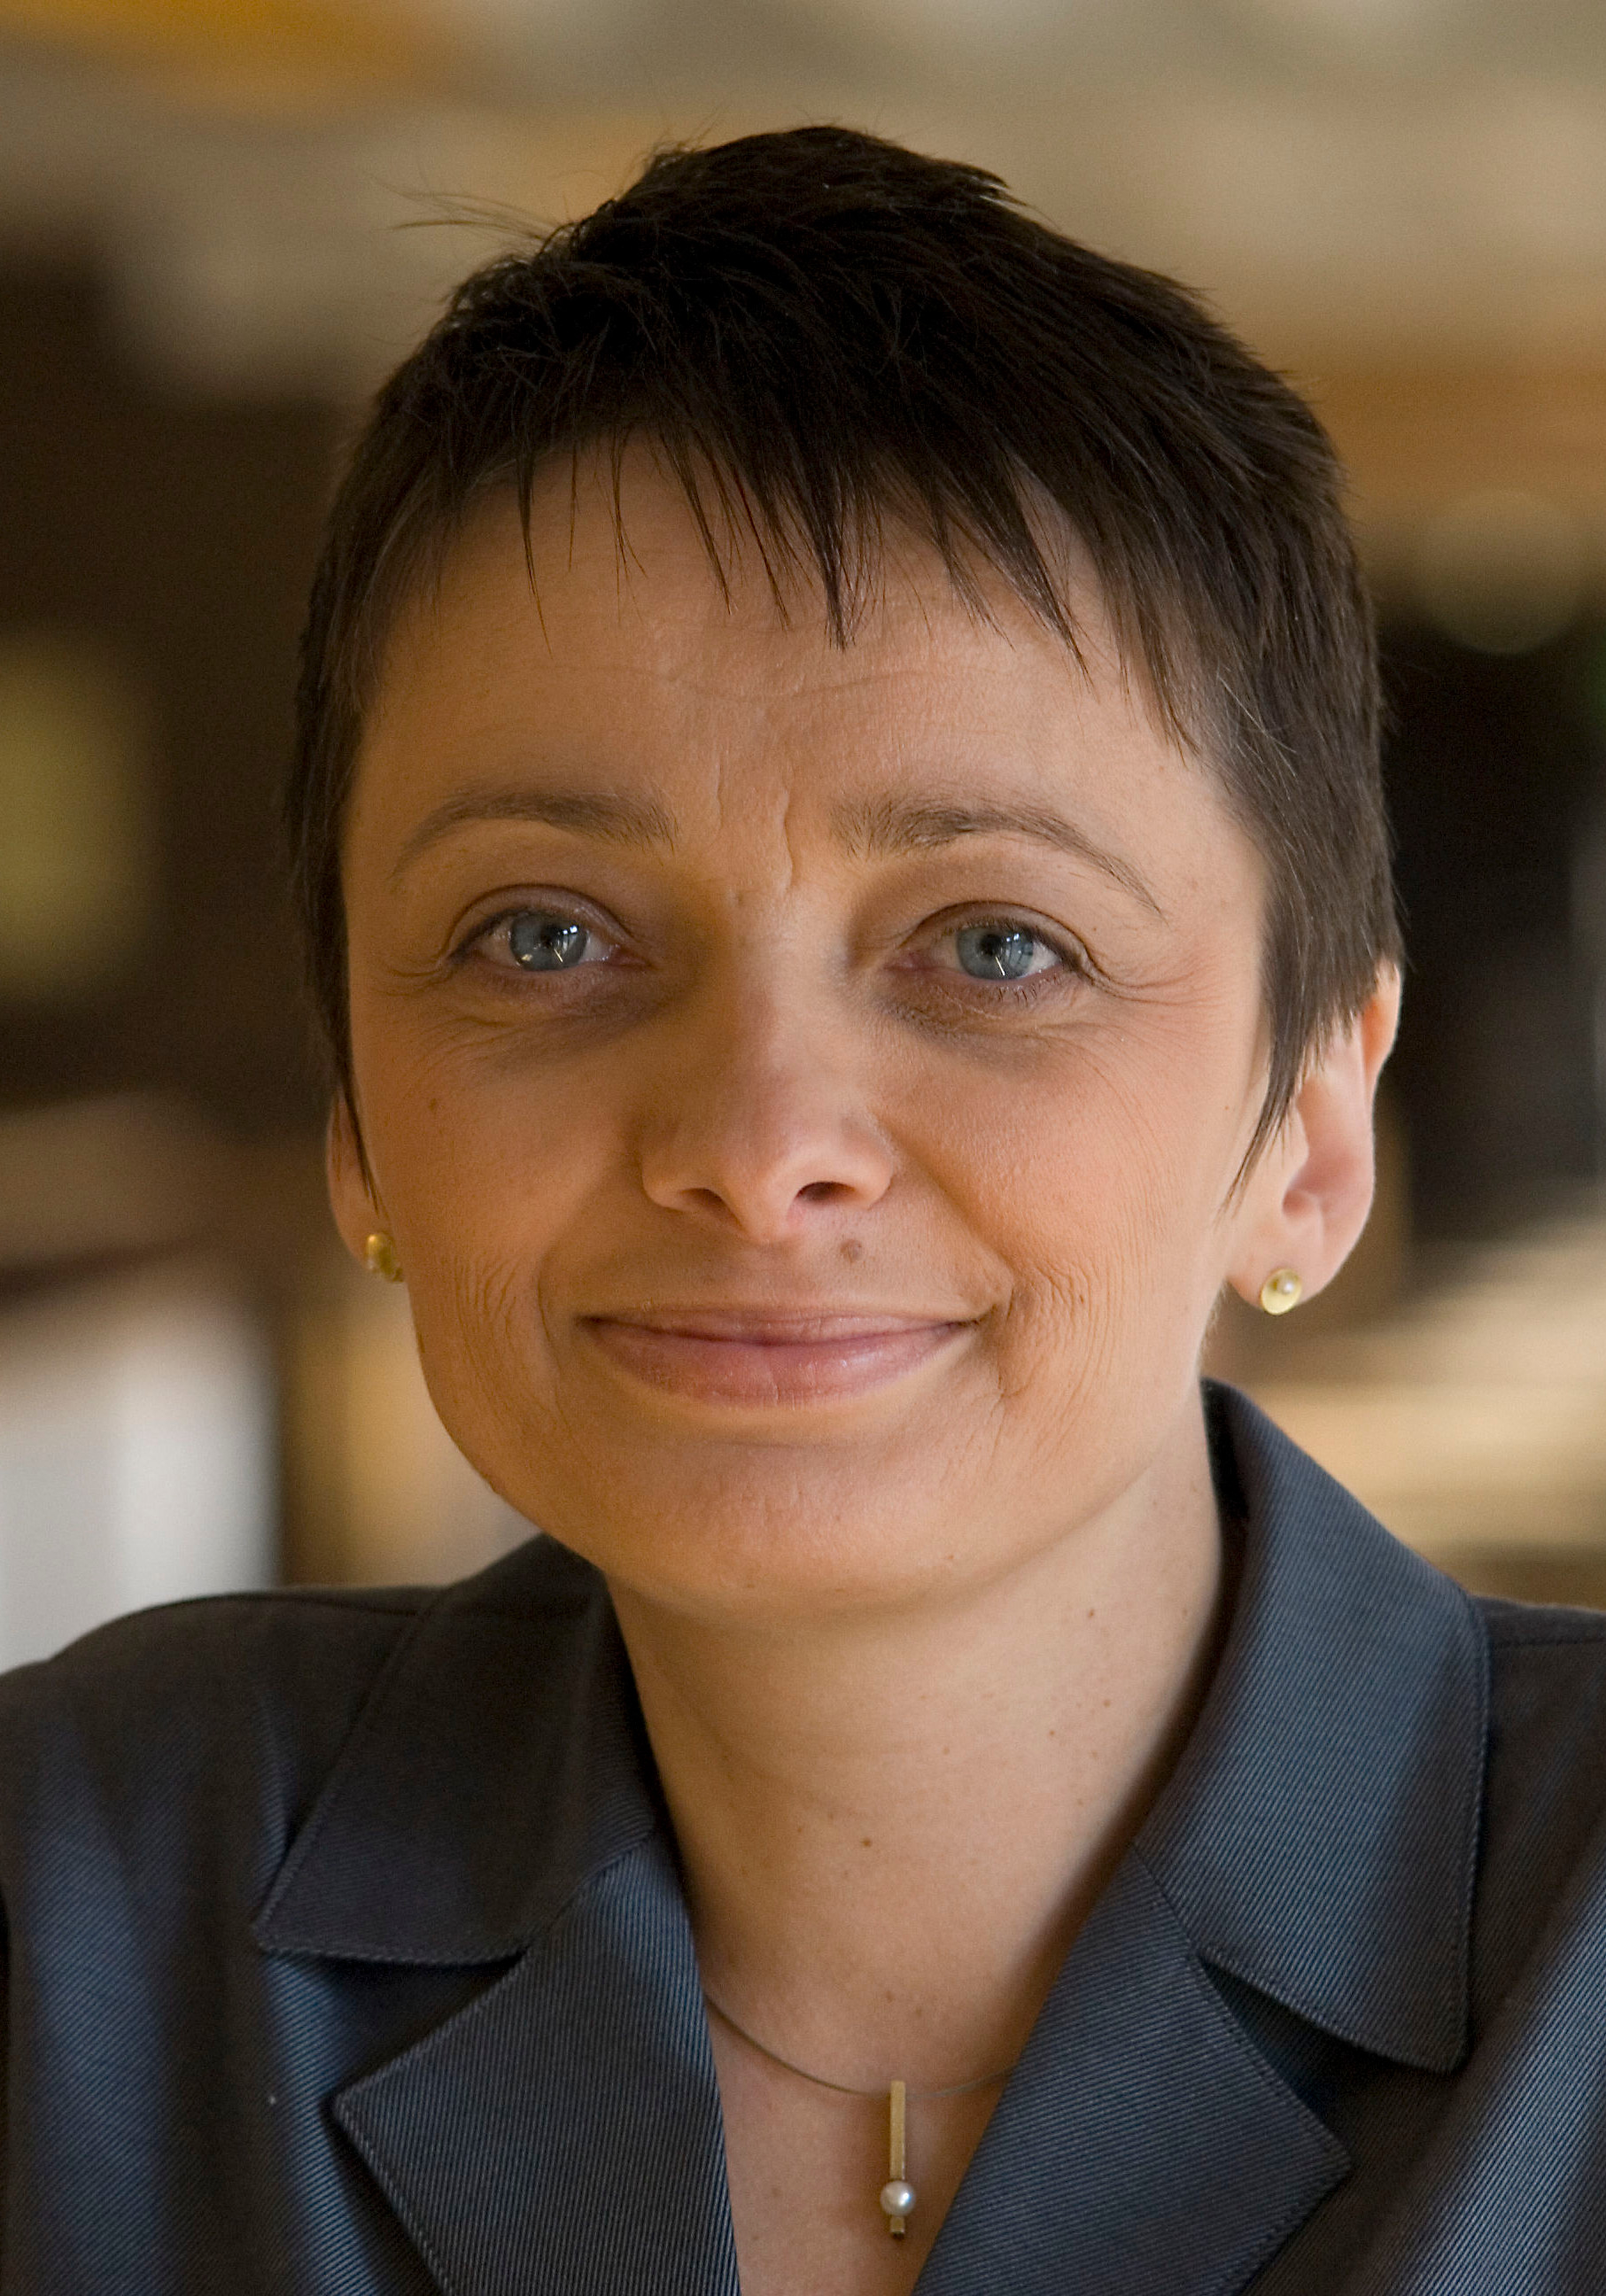
\includegraphics[height=0.25\textheight]{figures/erdmann.jpg} \\
%       Jeanette Erdmann \\
%     \end{column}
%     \begin{column}{0.4\textwidth}
%       \uncover<2->{
%       \center
%       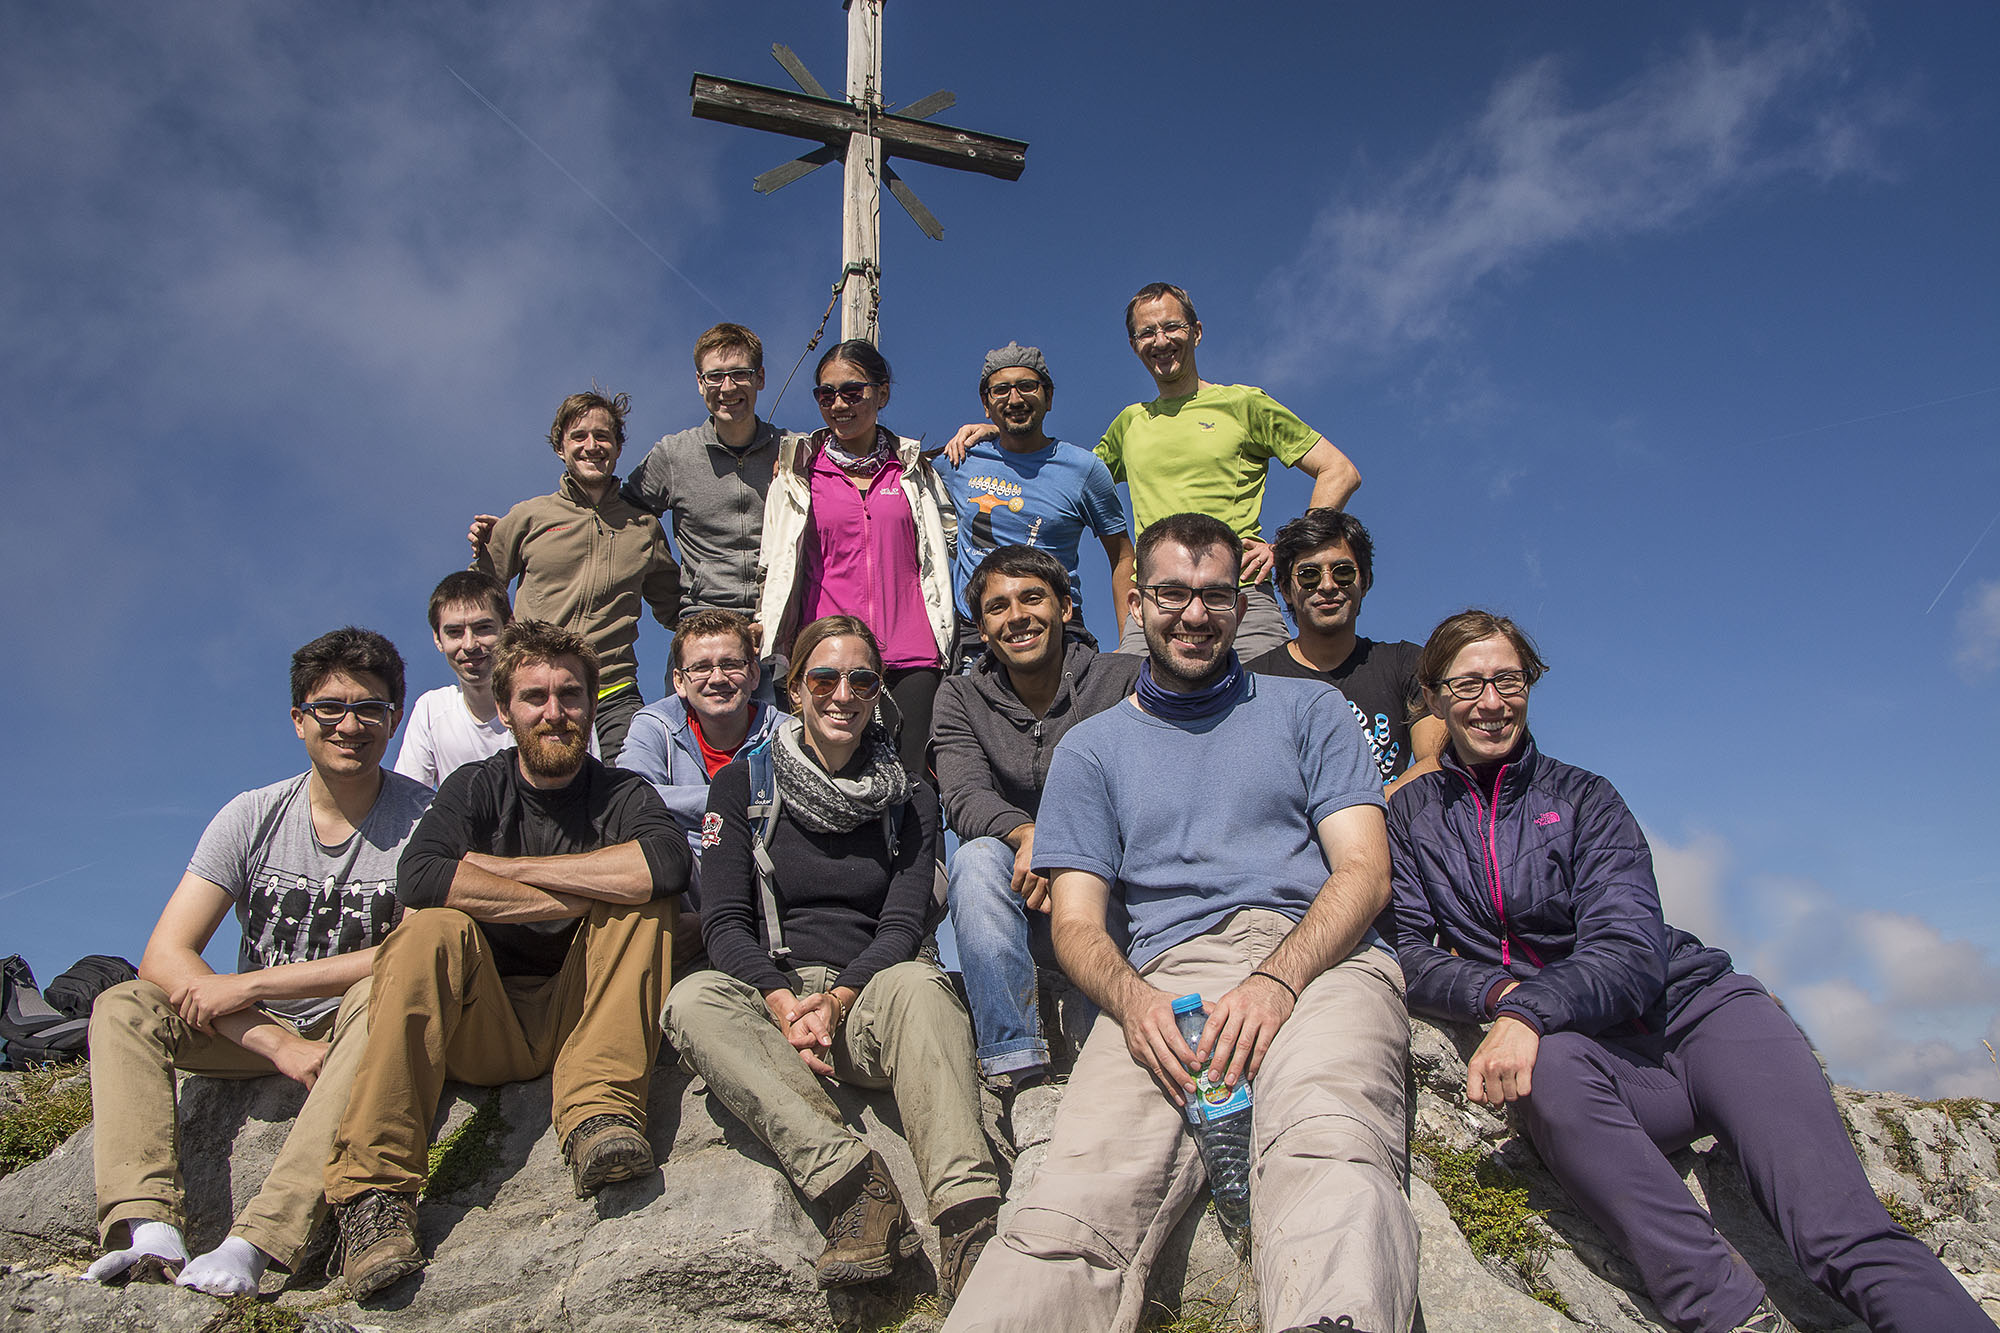
\includegraphics[width=1.0\textwidth]{figures/soeding_lab.jpg} \\
%       AG S\"oding \\
%       }
%     \end{column}
%   \end{columns}
%   \vskip0pt plus 1filll
%   \uncover<3->{
%   {\large  Thank you!}
%   }
%   \vskip0pt plus 1filll
%   \begin{columns}[c]
%     \begin{column}{0.25\textwidth}
%       
\includegraphics[height=0.11\textheight]{figures/emed_logo.png} \\
%     \end{column}
%     \begin{column}{0.25\textwidth}
%       
\includegraphics[height=0.11\textheight]{figures/eatherosysmed_logo.png} \\
%     \end{column}
%     \begin{column}{0.5\textwidth}
%       \hfill
%       Contact me: \\
%       \hfill
%       \textit{saikat.banerjee@mpibpc.mpg.de}
%       %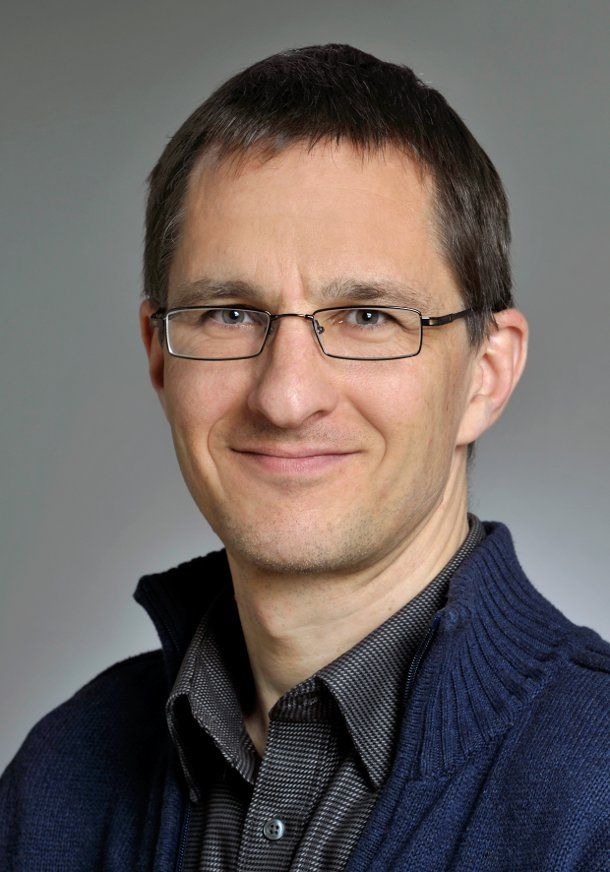
\includegraphics[height=0.3\textheight]{figures/soeding.jpg} \\
%     \end{column}
%   \end{columns}
% \end{frame}

%\begin{frame}
%  \frametitle{}
%\end{frame}

%\subsection{Appendix}
%
%\begin{frame}[noframenumbering]{Appendix A}
%\end{frame}

\end{document}
